
\write18{./make_talk.sh }

\documentclass[aspectratio=169]{beamer}
\usetheme{Pittsburgh}
\usecolortheme{spruce}
\usefonttheme{structurebold}
\beamertemplatenavigationsymbolsempty
\usepackage{graphicx}
\usepackage{tikz}
\usepackage{cite}
\usepackage{pgfpages}

%% \setbeameroption{hide notes}
\input{make.out}

\title{Far Flung Forest Landscapes in the Anthropocene}
\subtitle{Structural analysis of China's embodied forest network}
\author{Matthew Kekoa Lau (Ph.D.)}
\date{}
\institute{Chinese Academy of Sciences and Harvard University}


\begin{document}

{
\usebackgroundtemplate{
\begin{tikzpicture}[remember picture,overlay]
        \node[at=(current page.center), opacity=0.60]{
                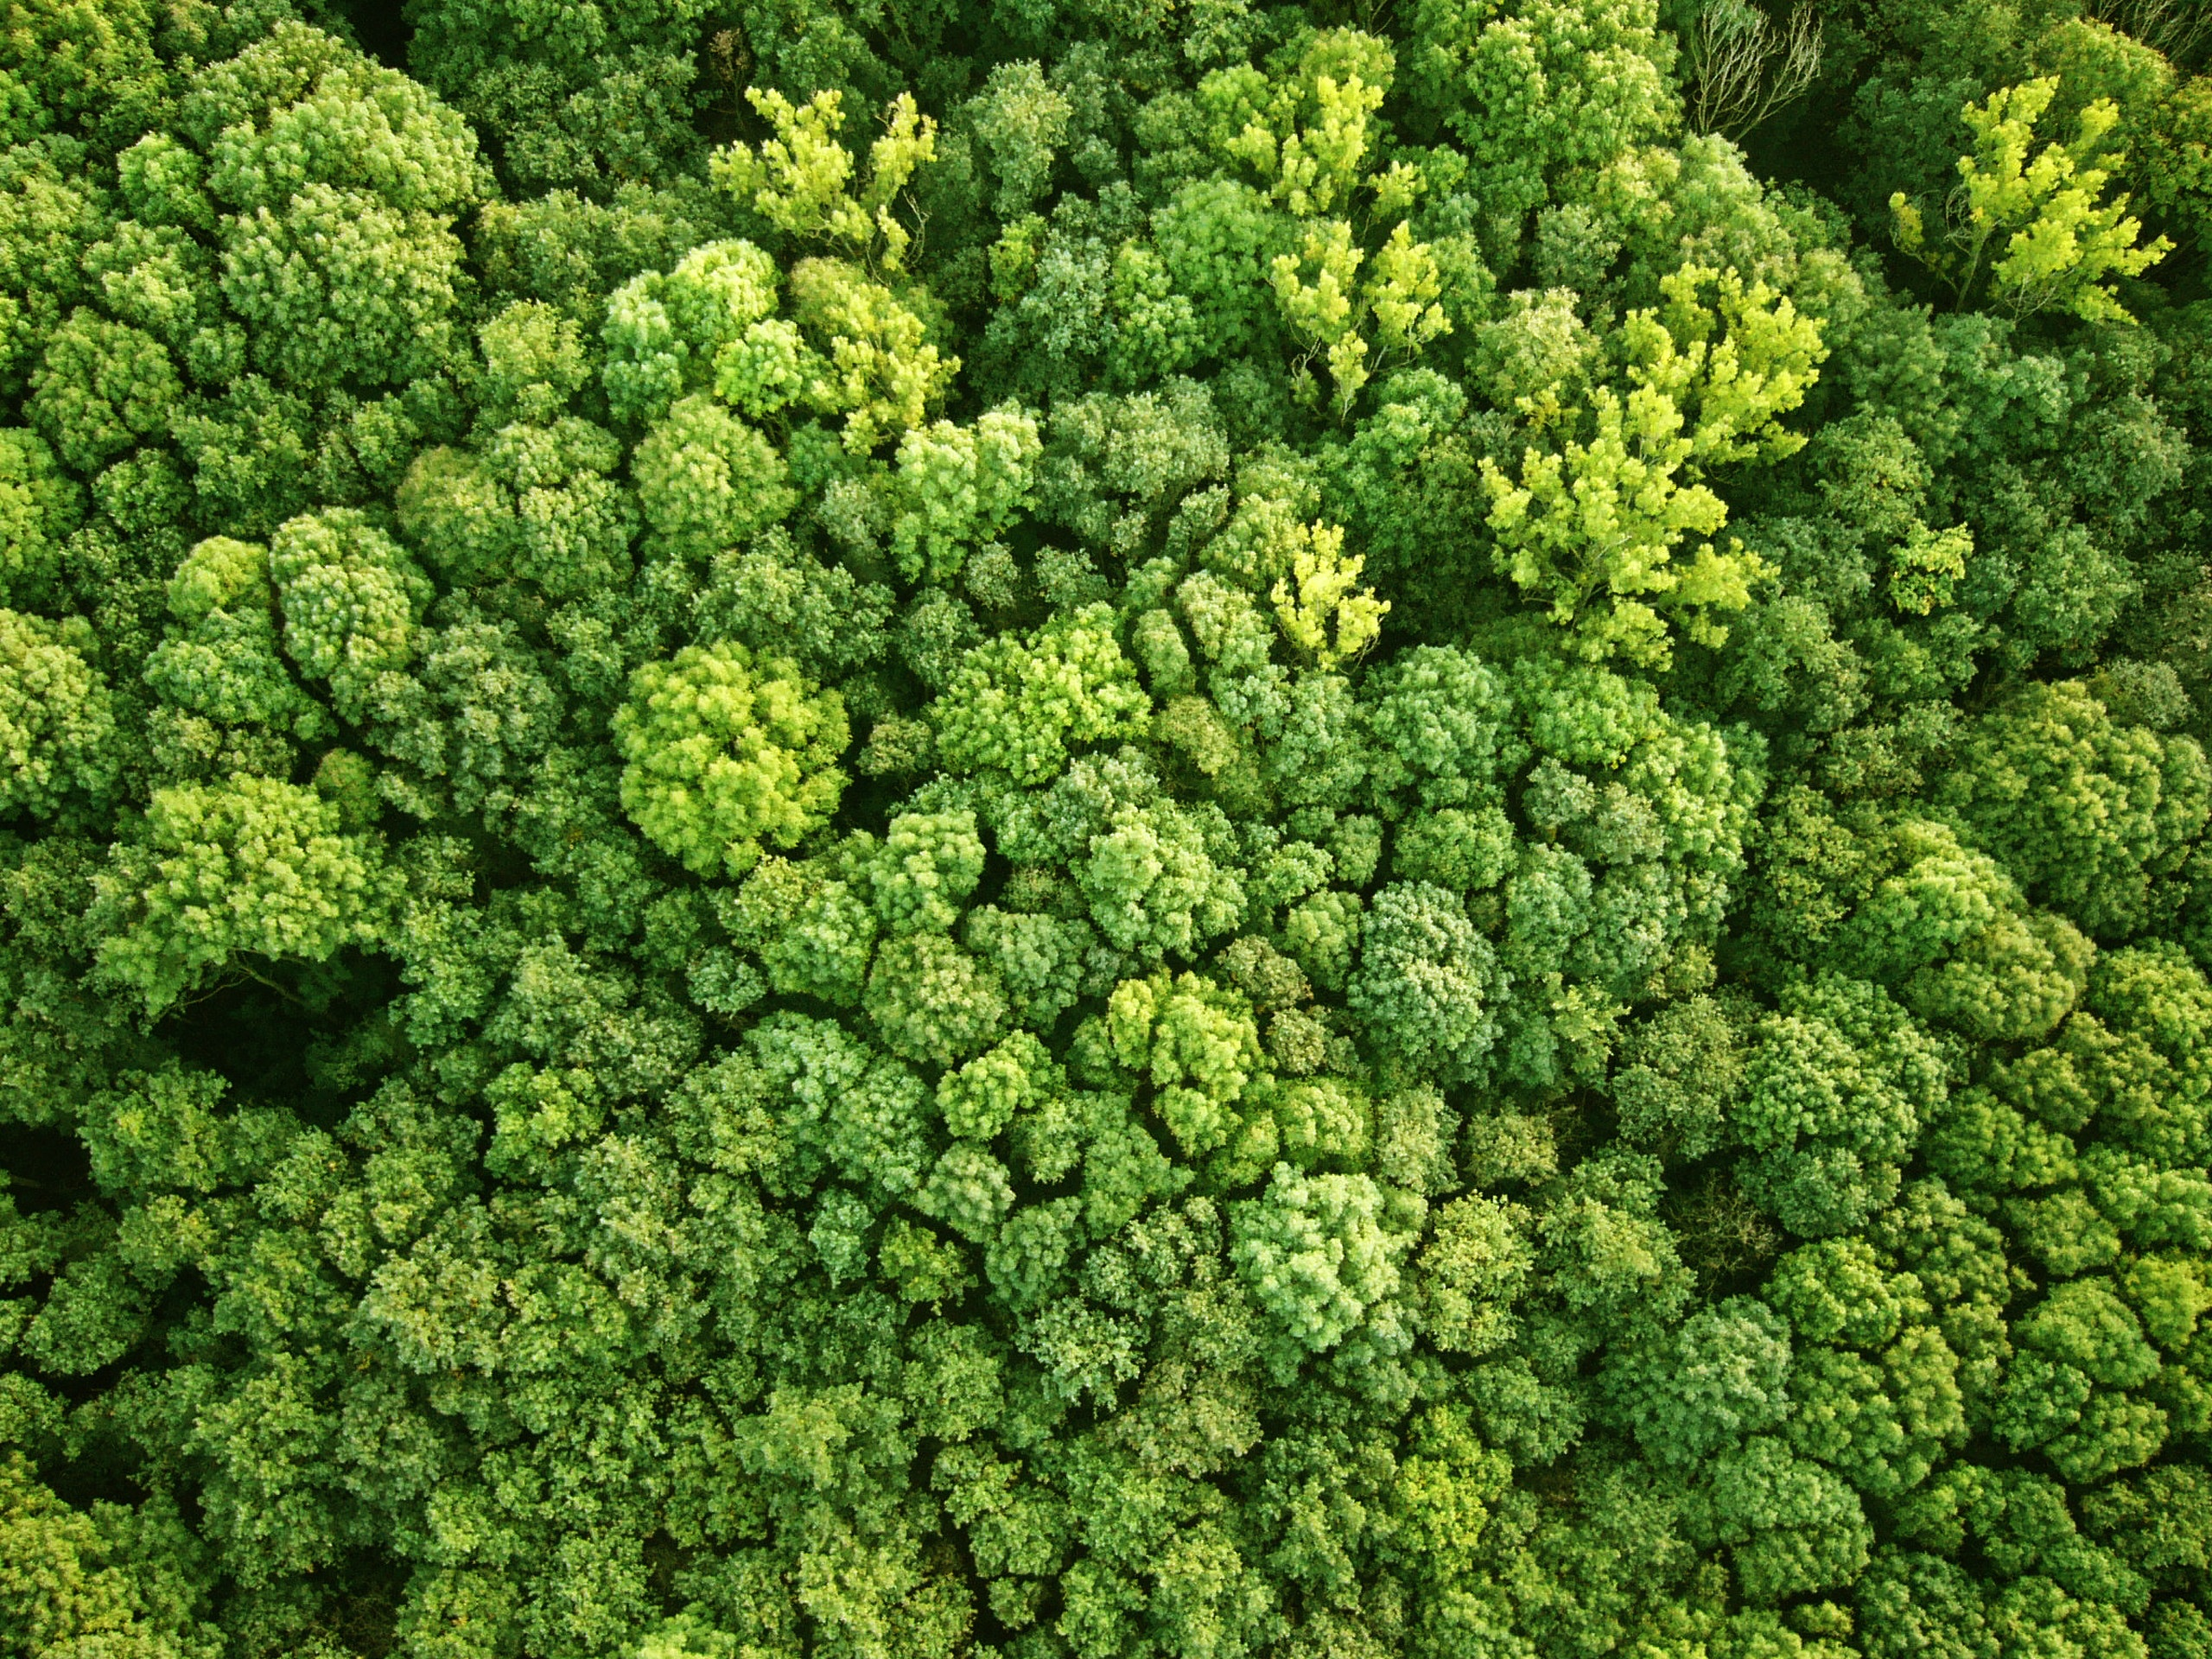
\includegraphics[keepaspectractio, width=\paperwidth]{images/forest_aerial.jpg}
        }
\end{tikzpicture}
}
\begin{frame}
  \titlepage
  \note[item]{Forests $\sim$ 80\% terrestrial biodiversity (WWF)}
  \note[item]{Forests carry out important processes: clean air and water}
  \note[item]{Forests store carbon}
\end{frame}
}

\section*{Context}

{ % all template changes are local to this group.
    \setbeamertemplate{navigation symbols}{}
    \begin{frame}<article:0>[plain]
      \frametitle{}
        \begin{tikzpicture}[remember picture,overlay]
            \node[at=(current page.center)] {
                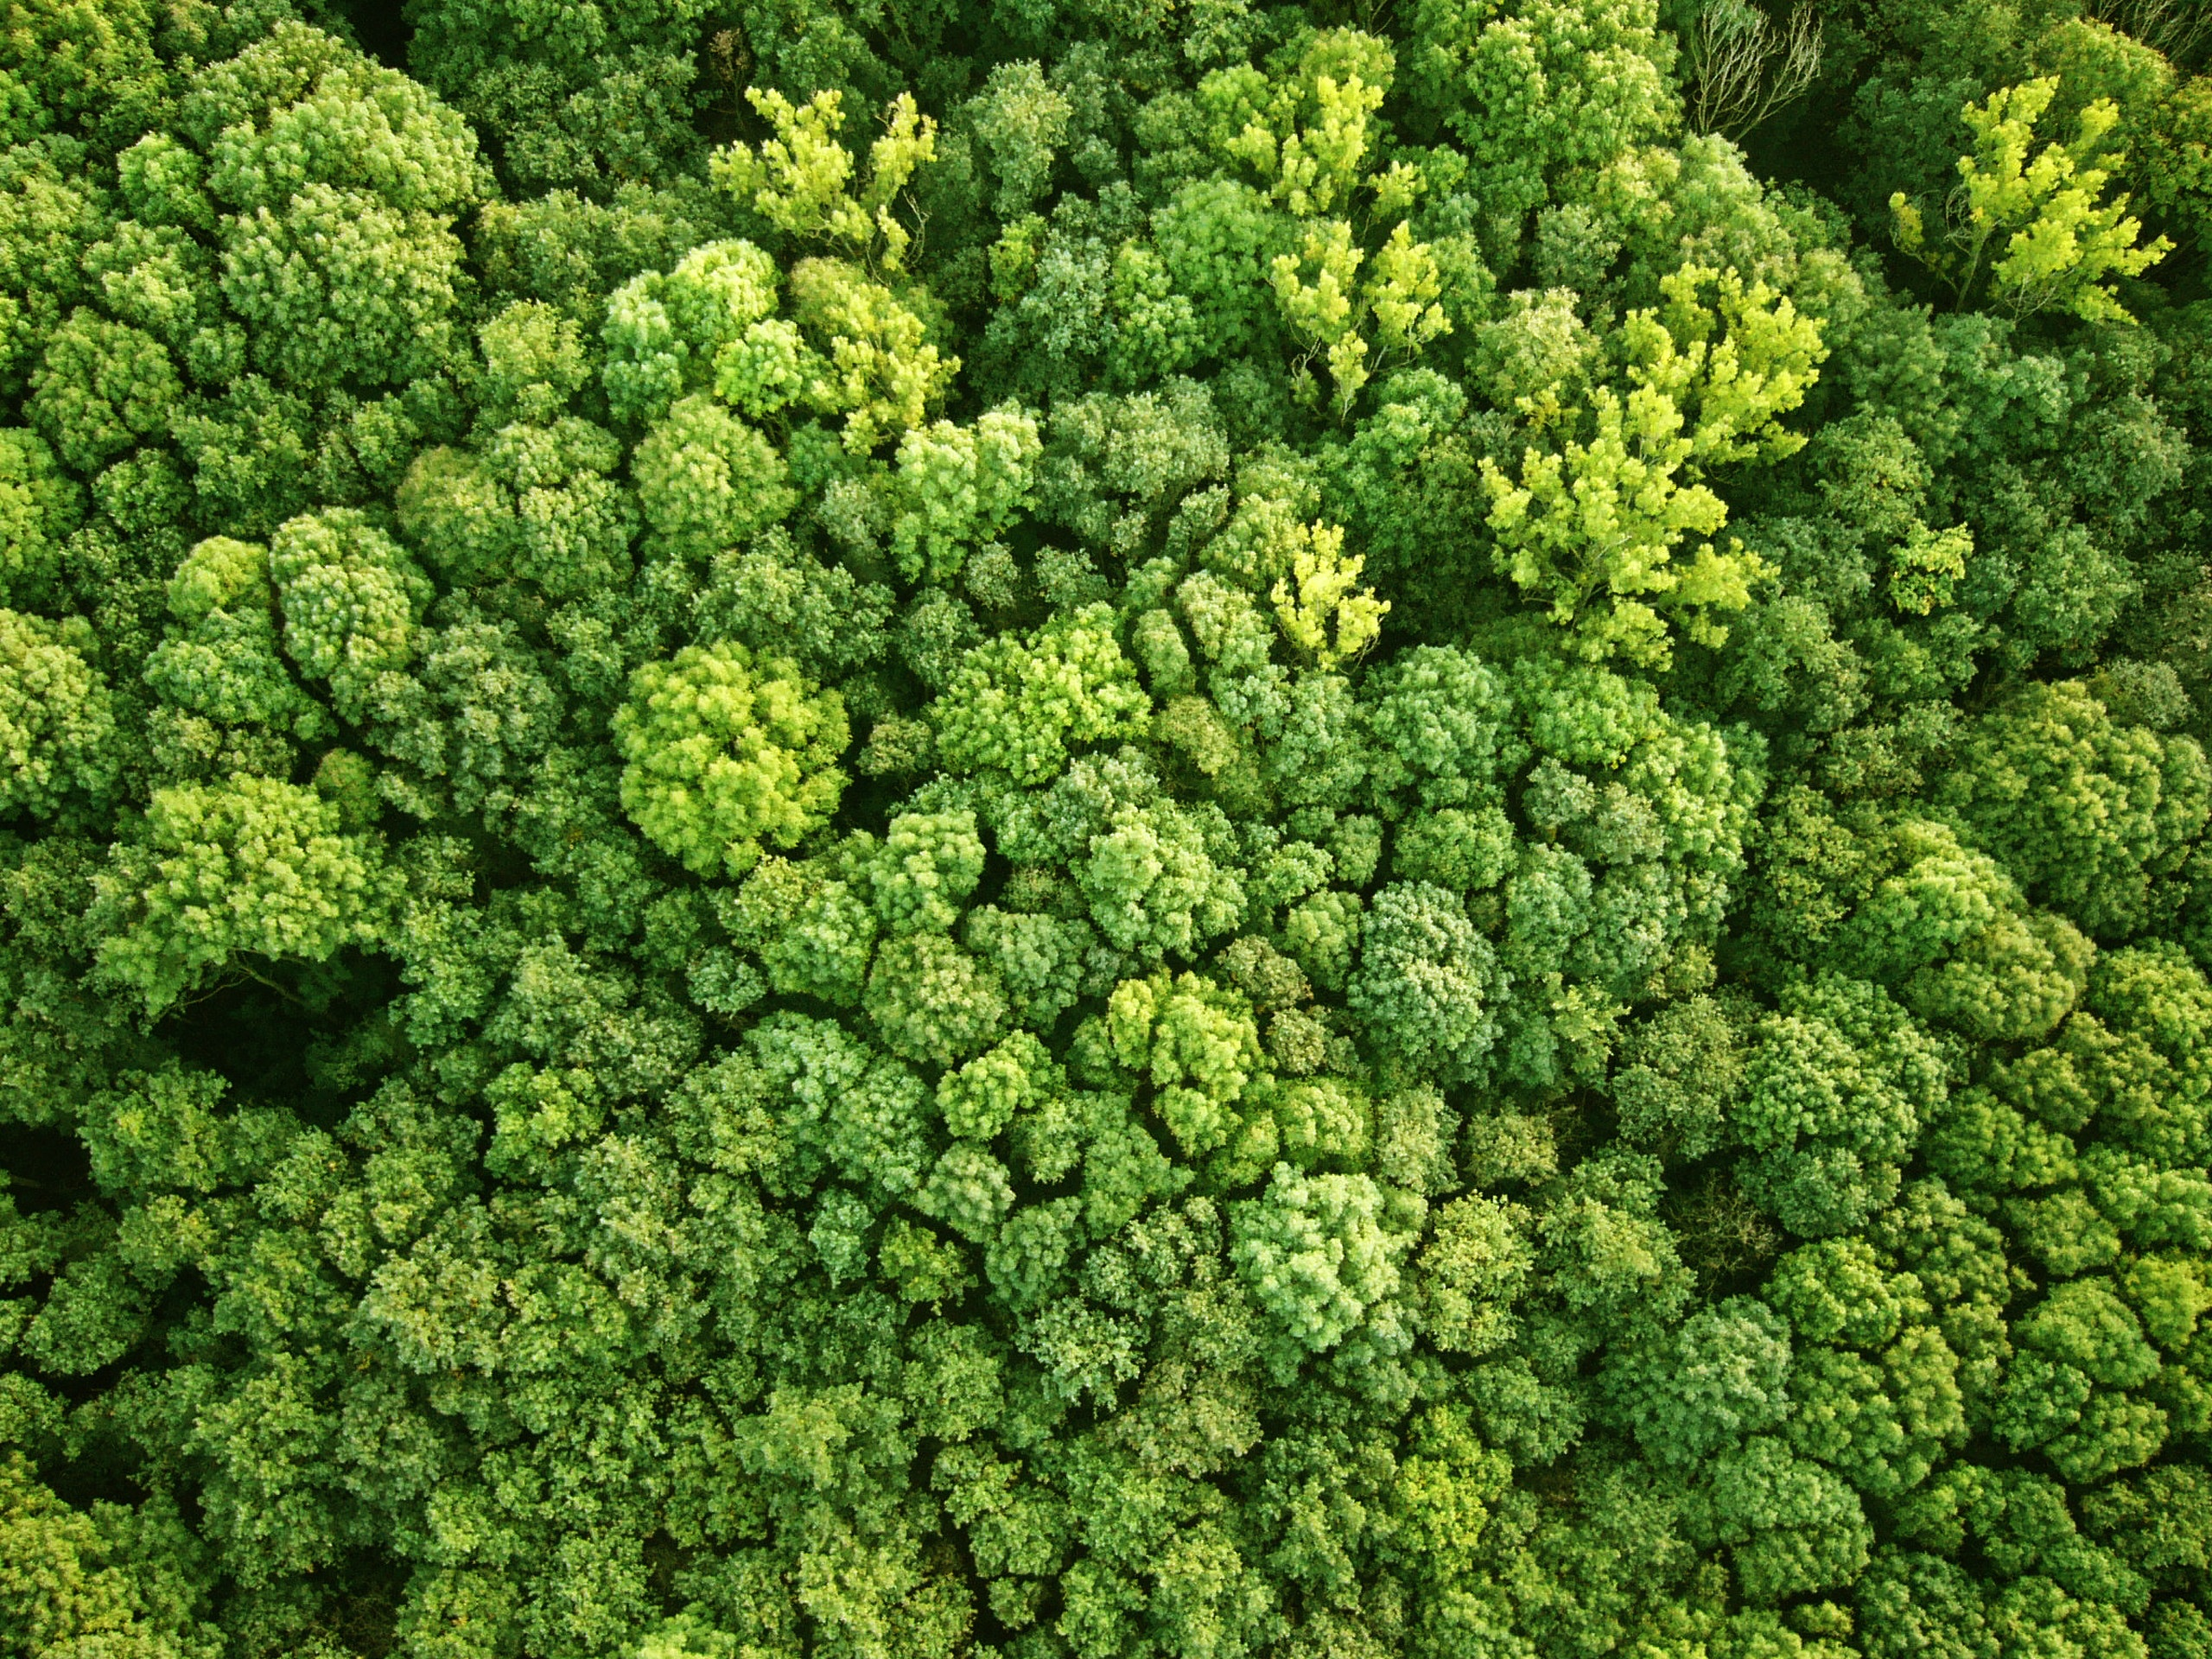
\includegraphics[keepaspectratio,
                                 width=\paperwidth]{images/forest_aerial.jpg}
            };
        \end{tikzpicture}
     \end{frame}
}

{ % all template changes are local to this group.
    \setbeamertemplate{navigation symbols}{}
    \begin{frame}<article:0>[plain]
      \frametitle{}
        \begin{tikzpicture}[remember picture,overlay]
            \node[at=(current page.center)] {
                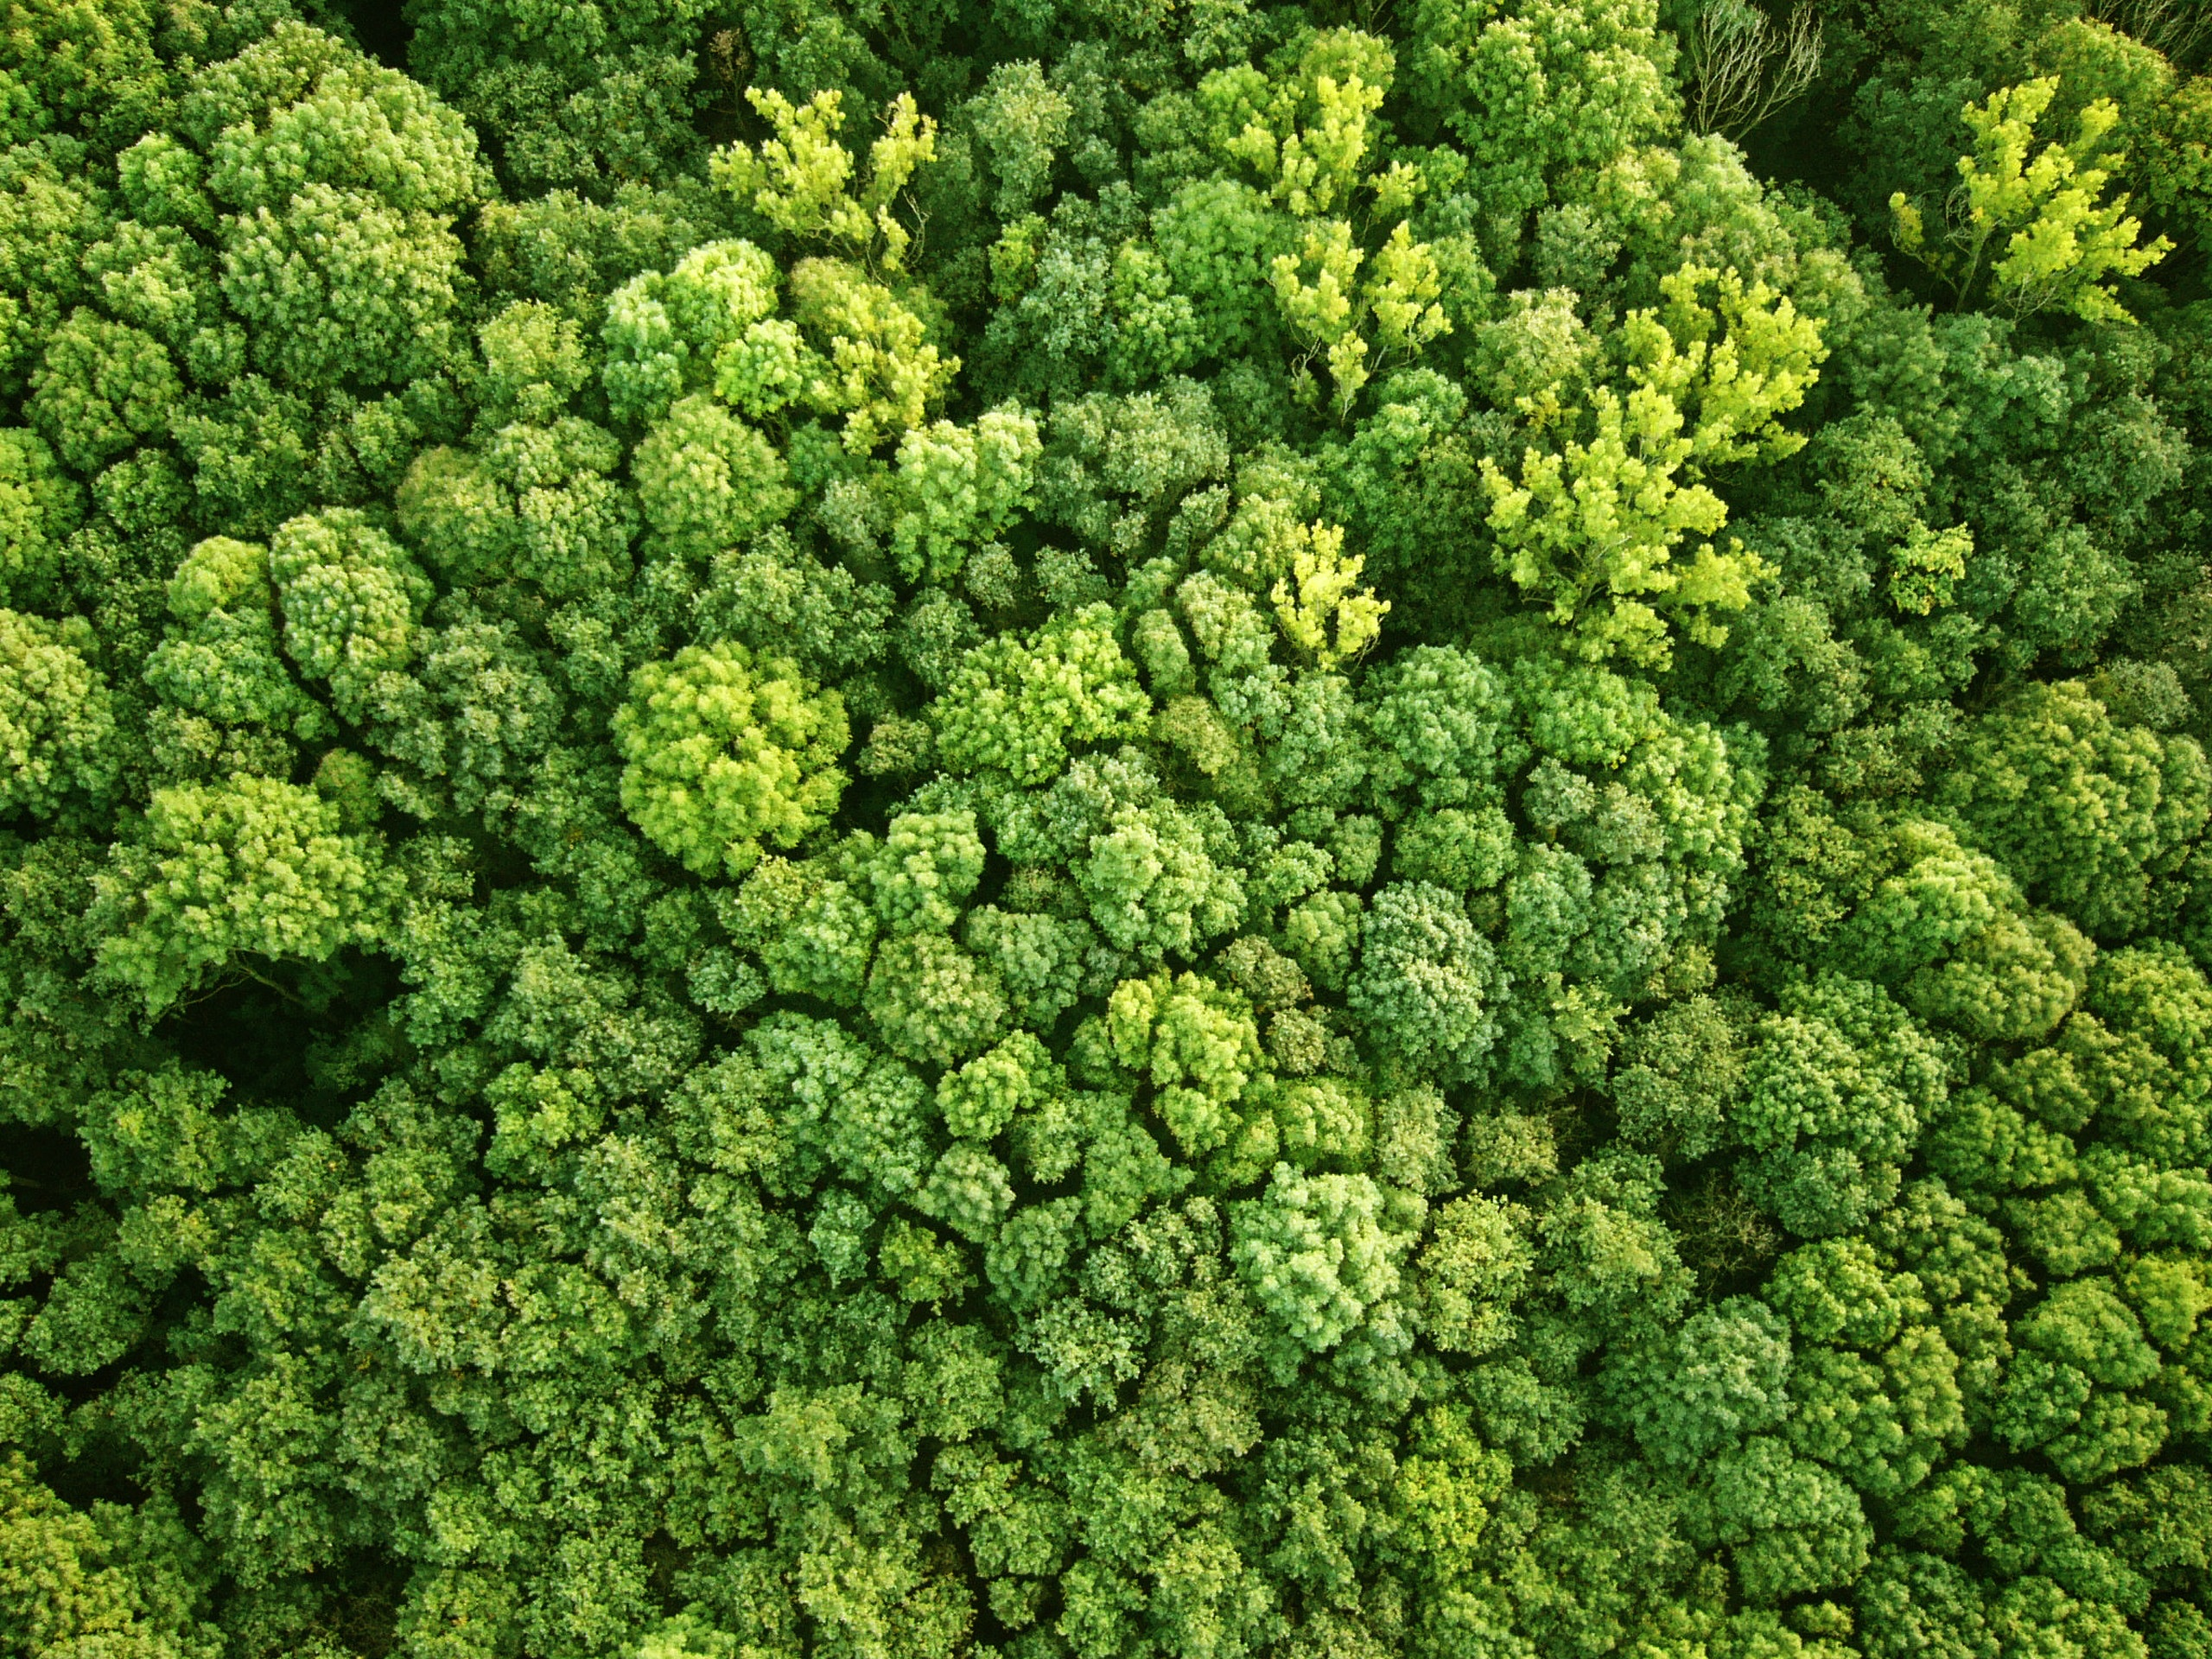
\includegraphics[keepaspectratio,
                                 width=\paperwidth]{images/forest_aerial.jpg}
            };
            \node[at=(current page.center)] {
                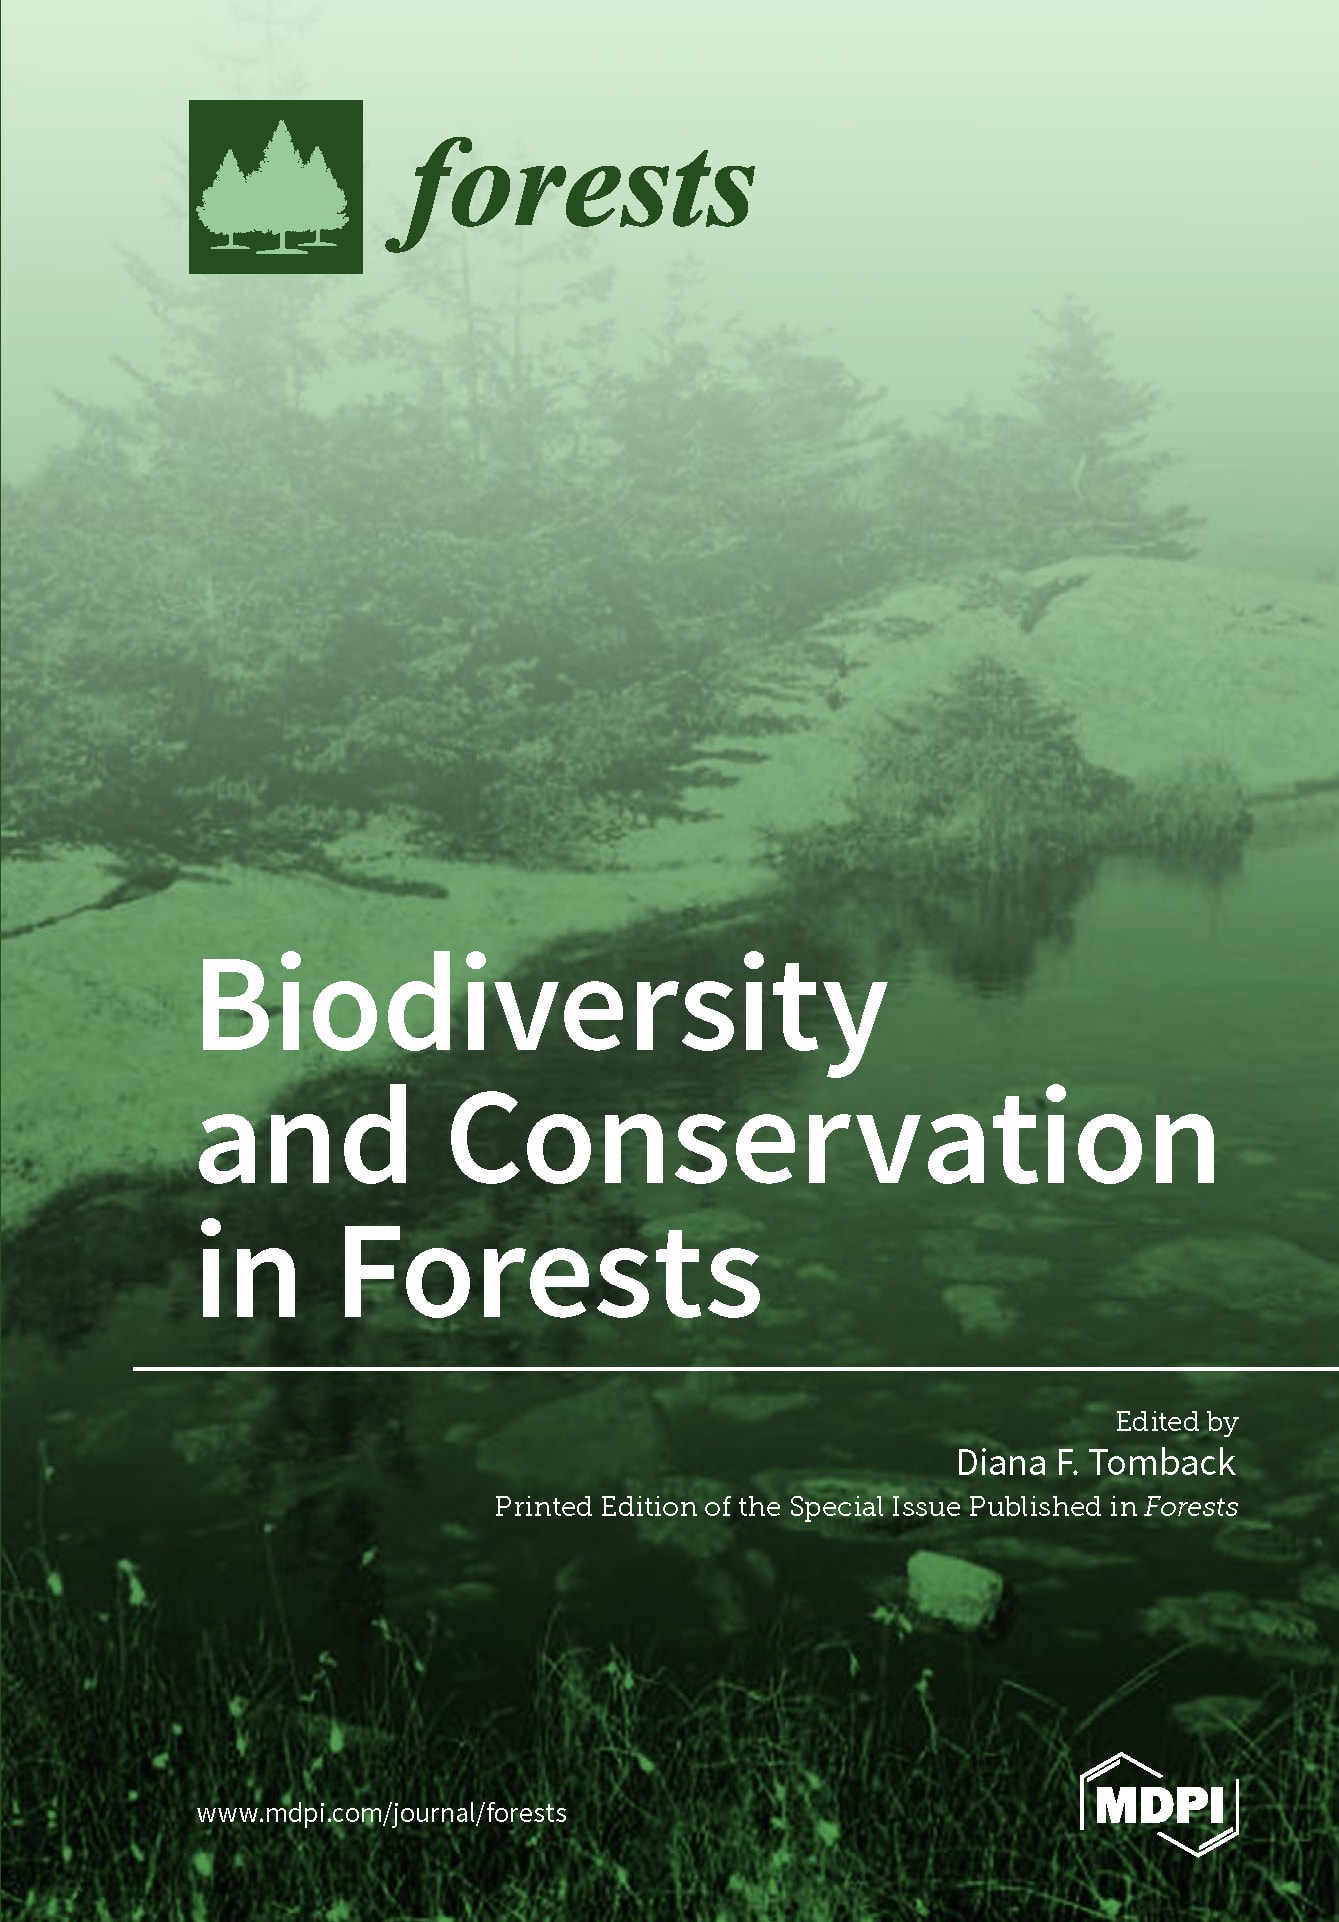
\includegraphics[keepaspectratio,
                                 height=\paperheight]{images/forest_biodiversity.jpg}
            };
        \end{tikzpicture}
     \end{frame}
}


{ % all template changes are local to this group.
    \setbeamertemplate{navigation symbols}{}
    \begin{frame}<article:0>[plain]
      \frametitle{}
        \begin{tikzpicture}[remember picture,overlay]
            \node[at=(current page.center)] {
                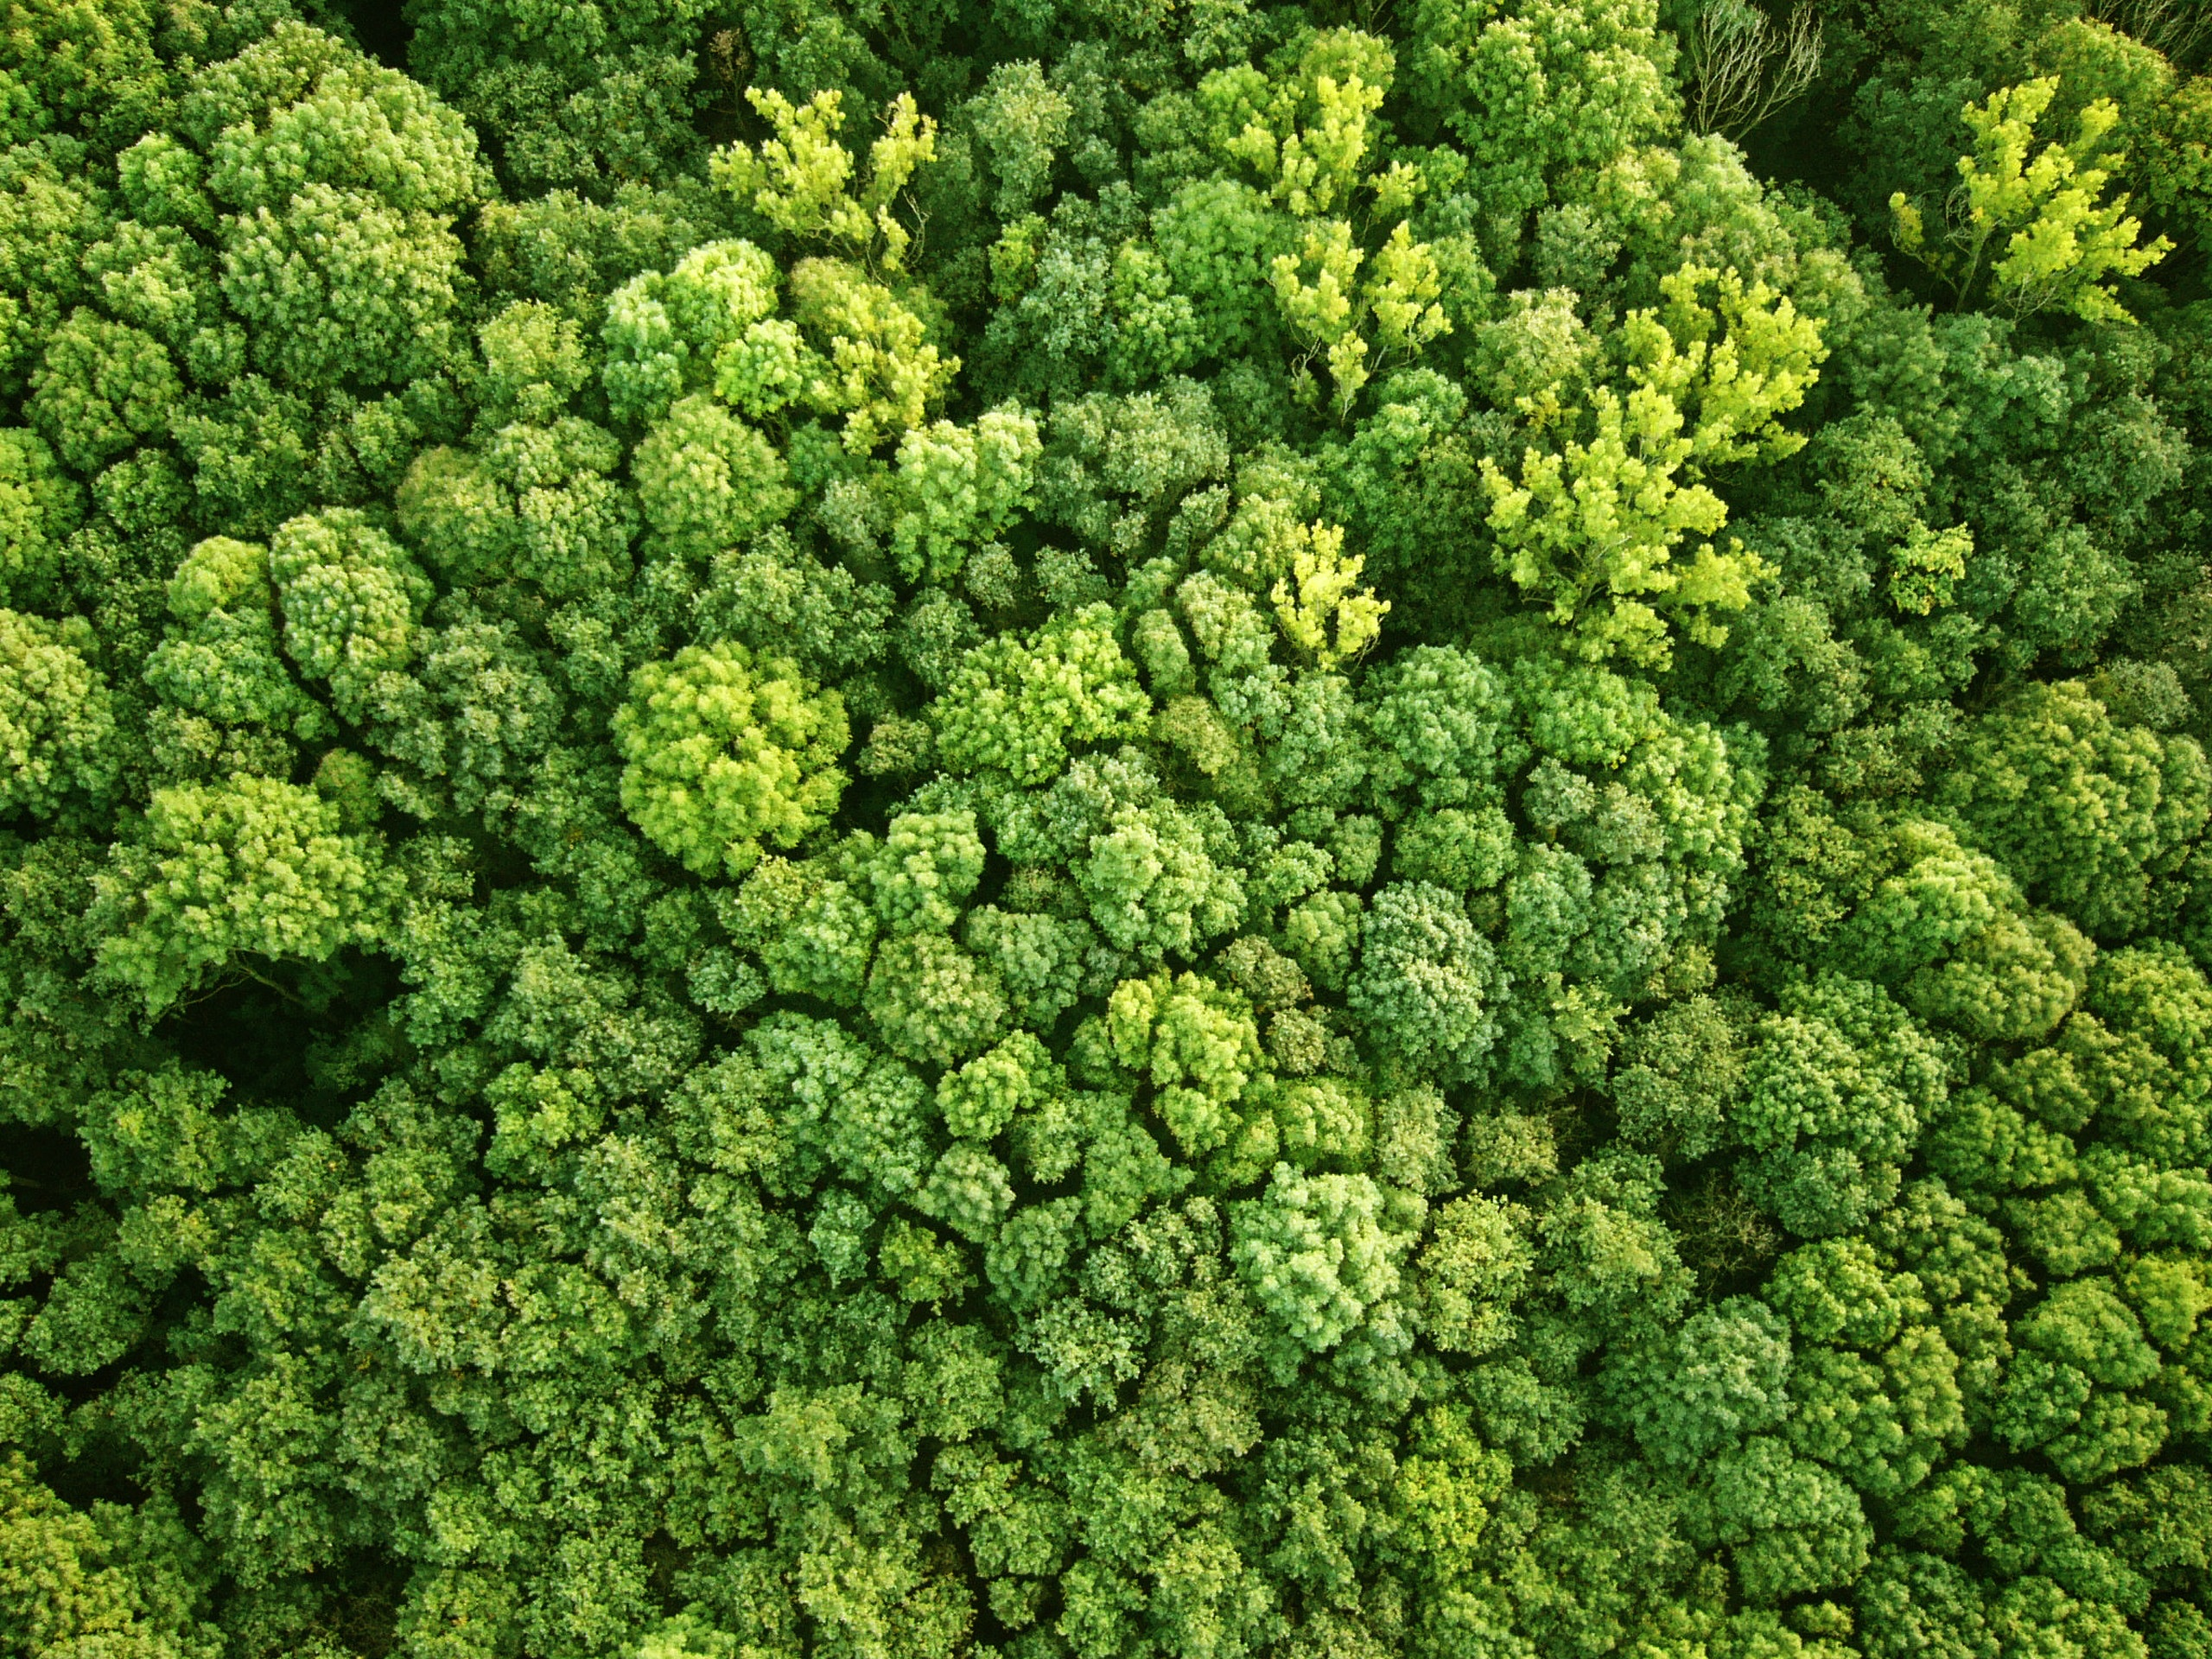
\includegraphics[keepaspectratio,
                                 width=\paperwidth]{images/forest_aerial.jpg}
            };
            \node[at=(current page.center)] {
                
\includegraphics[keepaspectratio,
                                 height=\paperheight]{images/glass-of-water.jpg}
            };
        \end{tikzpicture}
     \end{frame}
}


{ % all template changes are local to this group.
    \setbeamertemplate{navigation symbols}{}
    \begin{frame}<article:0>[plain]
      \frametitle{}
        \begin{tikzpicture}[remember picture,overlay]
            \node[at=(current page.center)] {
                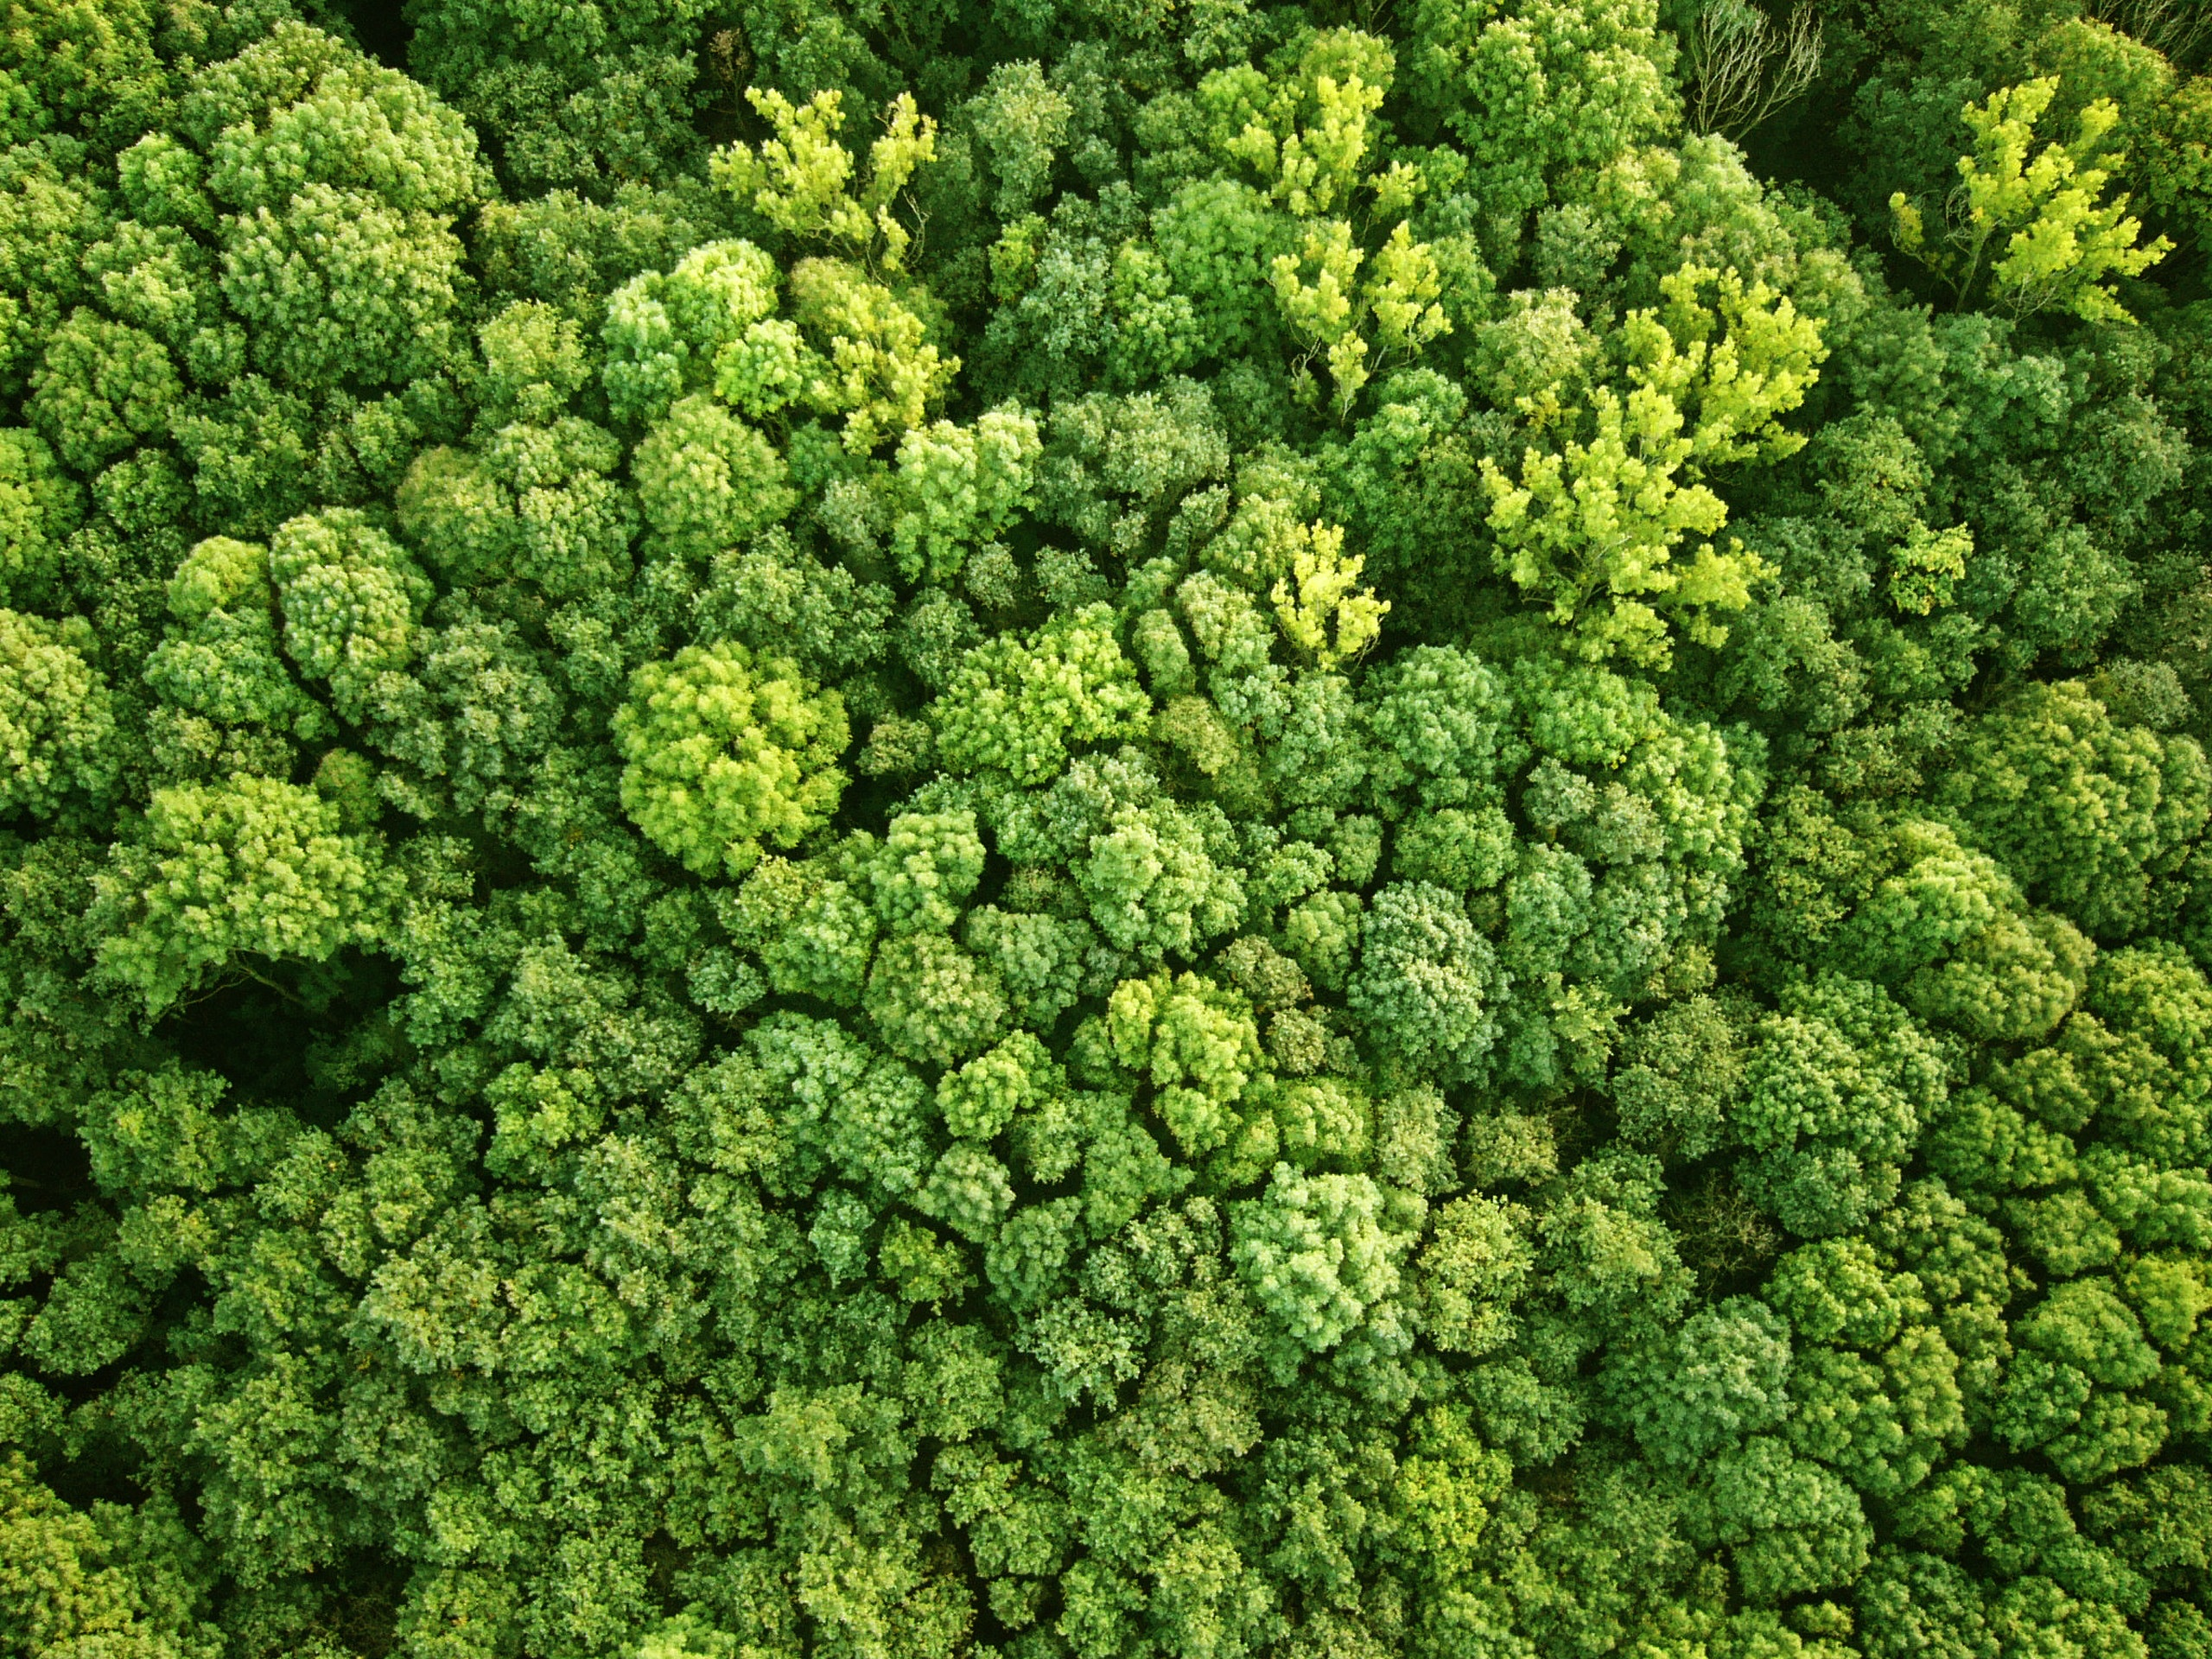
\includegraphics[keepaspectratio,
                                 width=\paperwidth]{images/forest_aerial.jpg}
            };
            \node[at=(current page.center)] {
                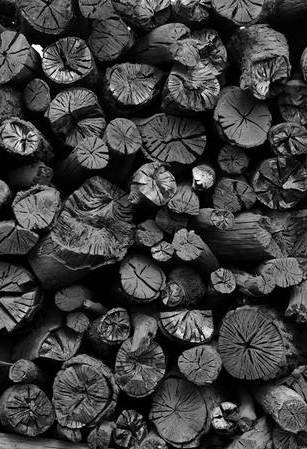
\includegraphics[keepaspectratio,
                                 height=\paperheight]{images/carbon.jpg}
            };
        \end{tikzpicture}
     \end{frame}
}


{ % all template changes are local to this group.
    \setbeamertemplate{navigation symbols}{}
    \begin{frame}<article:0>[plain]
      \frametitle{}
        \begin{tikzpicture}[remember picture,overlay]
            \node[at=(current page.center)] {
                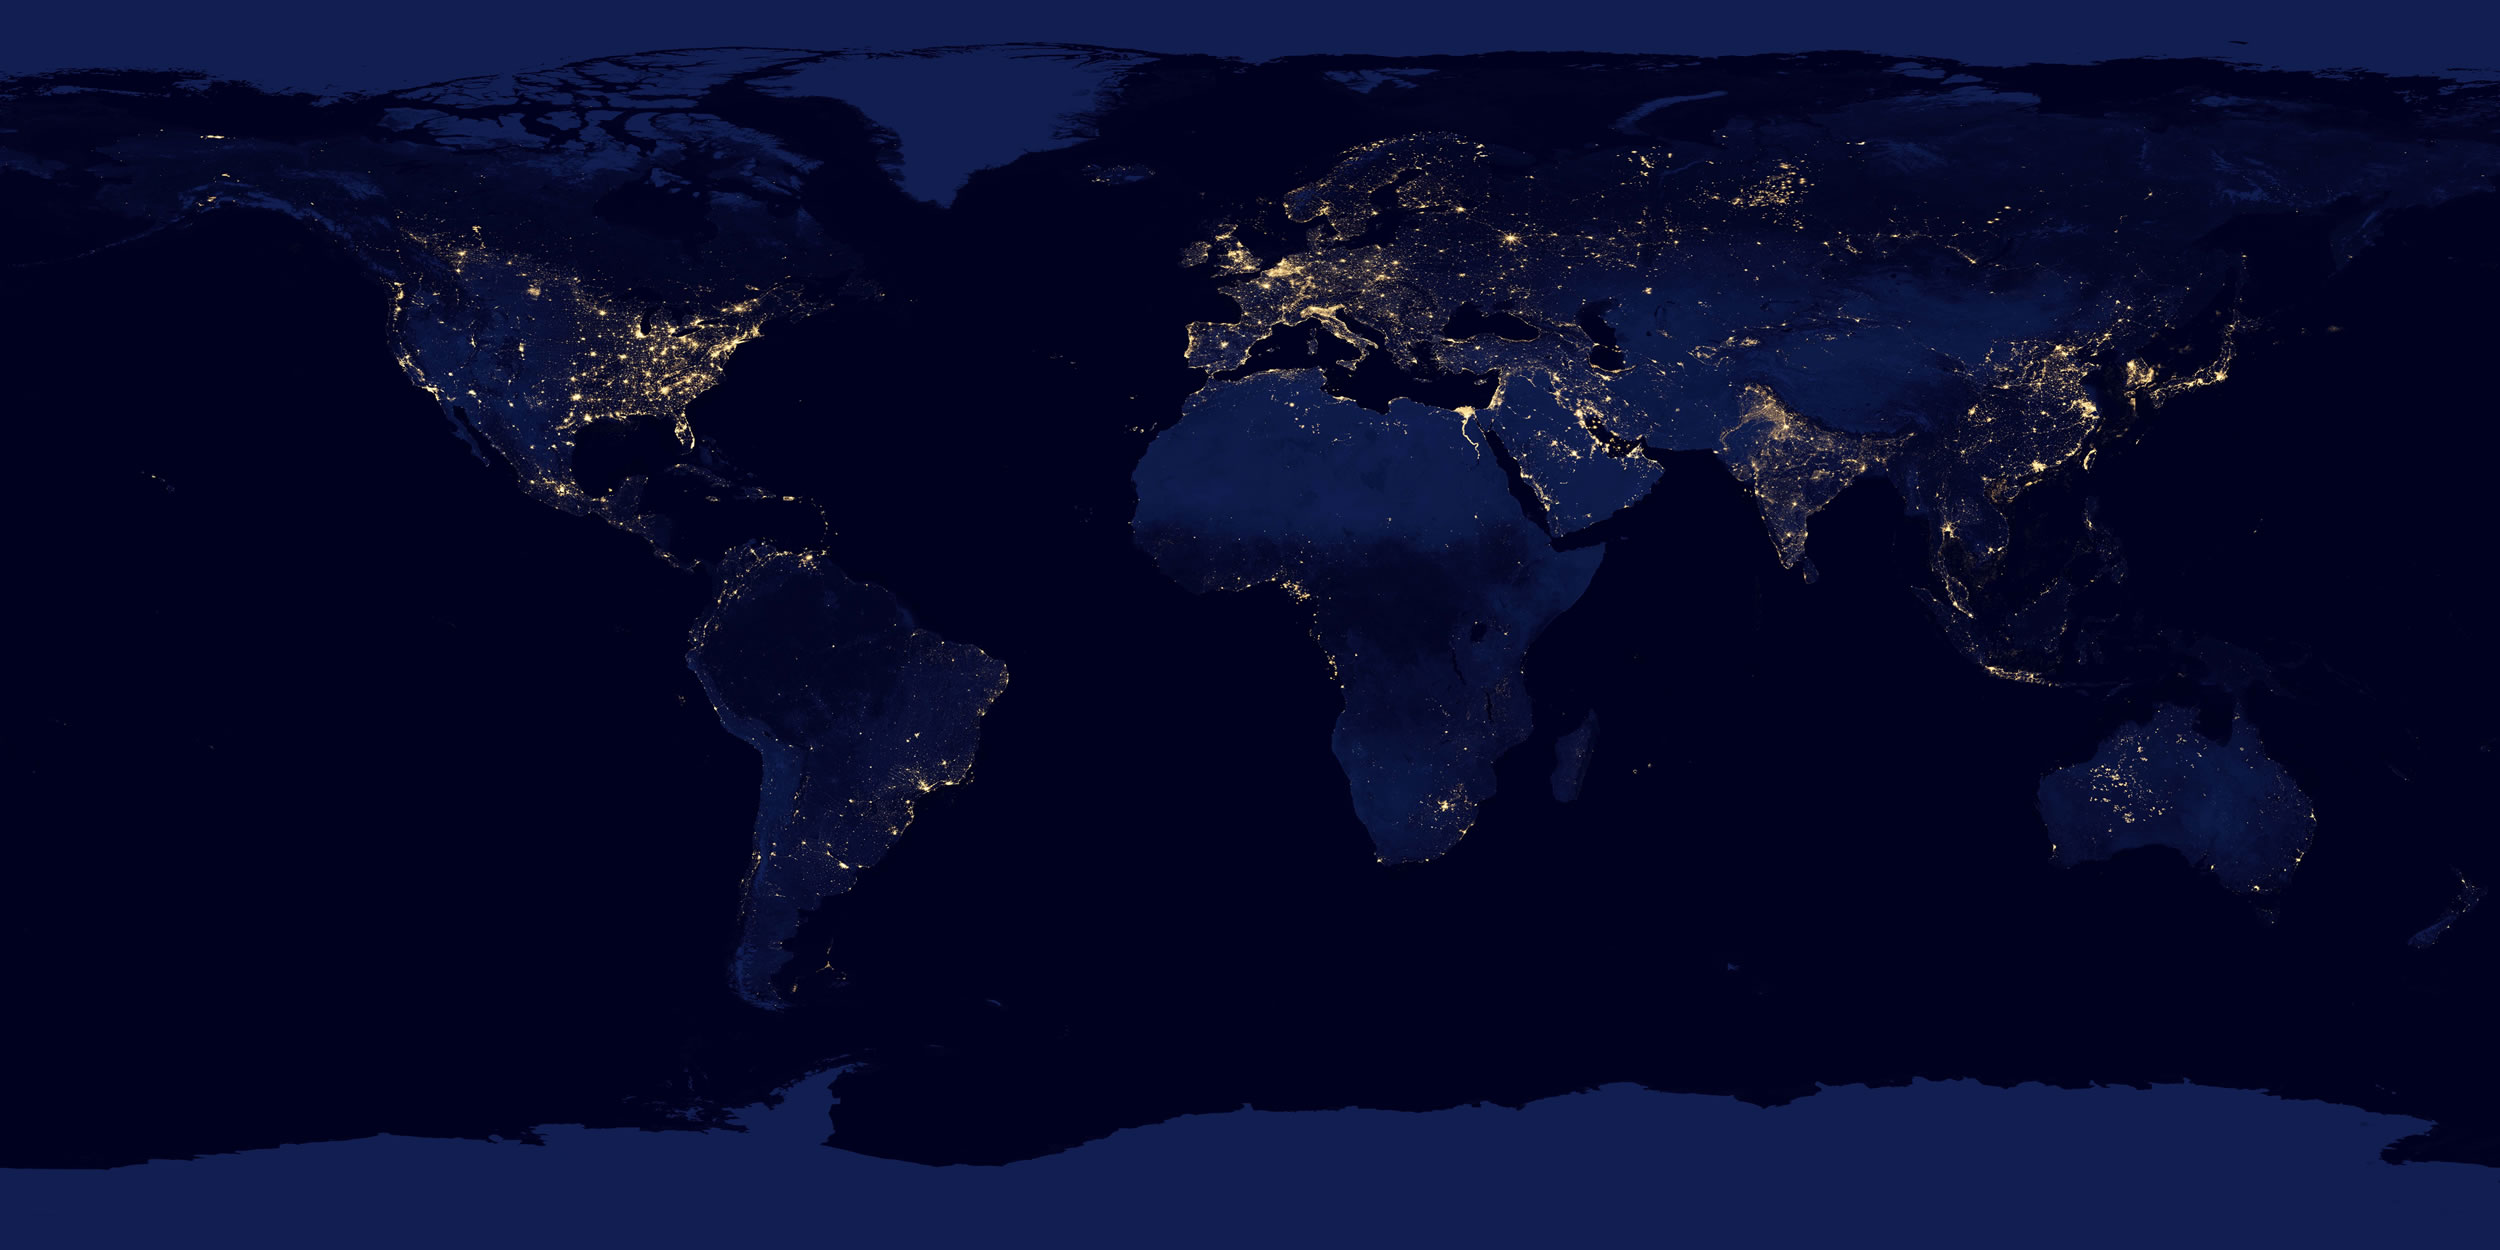
\includegraphics[keepaspectratio,
                                 height=\paperheight]{images/satellite-view-of-earth-at-night.jpg}
            };
        \end{tikzpicture}
  \note[item]{Anthropocene = proposed geological epoch distinguished by human impacts}
     \end{frame}
}



{ % all template changes are local to this group.
    \setbeamertemplate{navigation symbols}{}
    \begin{frame}<article:0>[plain]
      \frametitle{}
      \cite{Ellis2020AnthropogenicCE}
        \begin{tikzpicture}[remember picture,overlay]
            \node[at=(current page.center)] {
                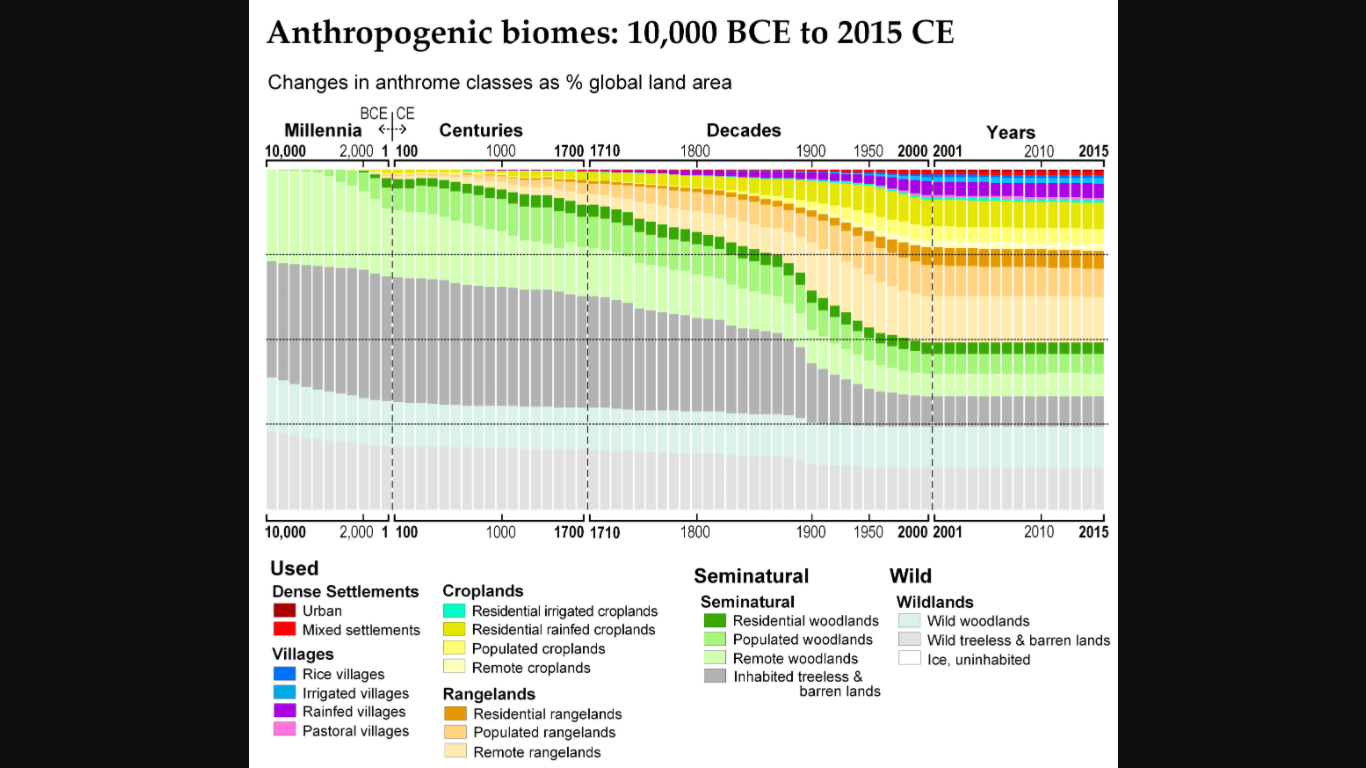
\includegraphics[keepaspectratio,
                                 width=\paperwidth,
                                 scale=0.25]{images/anthromes.png}
            };
        \end{tikzpicture}
  \note[item]{Land-use changes = conversion}
  \note[item]{One proposal is it started about 1950 with acceleration}
  \note[item]{Biodiversity changes = species introductions and extinctions}
     \end{frame}
}

{ % all template changes are local to this group.
    \setbeamertemplate{navigation symbols}{}
    \begin{frame}<article:0>[plain]
      \frametitle{}
        \begin{tikzpicture}[remember picture,overlay]
            \node[at=(current page.center)] {
                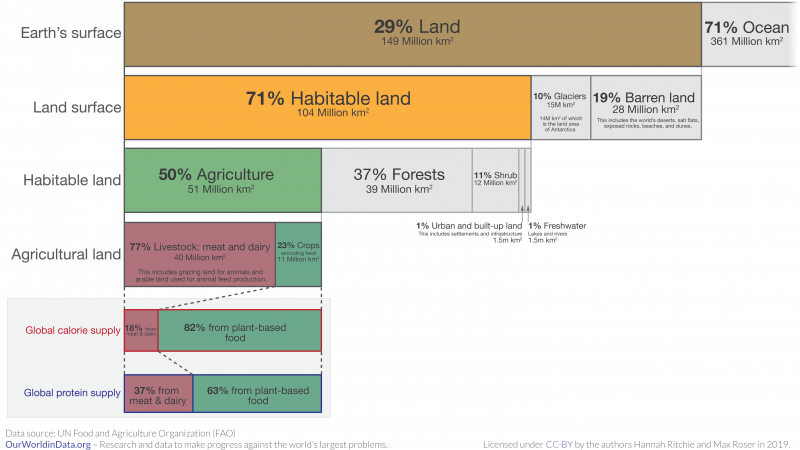
\includegraphics[keepaspectratio,
                                 width=\paperwidth,
                                 scale=0.25]{images/Global-land-use-graphic-800x506.png}
            };
        \end{tikzpicture}
  \note[item]{90\% biomass on Earth is humans and livestock}
     \end{frame}
}


{ % all template changes are local to this group.
    \setbeamertemplate{navigation symbols}{}
    \begin{frame}<article:0>[plain]
      \frametitle{}
        \begin{tikzpicture}[remember picture,overlay]
            \node[at=(current page.center)] {
                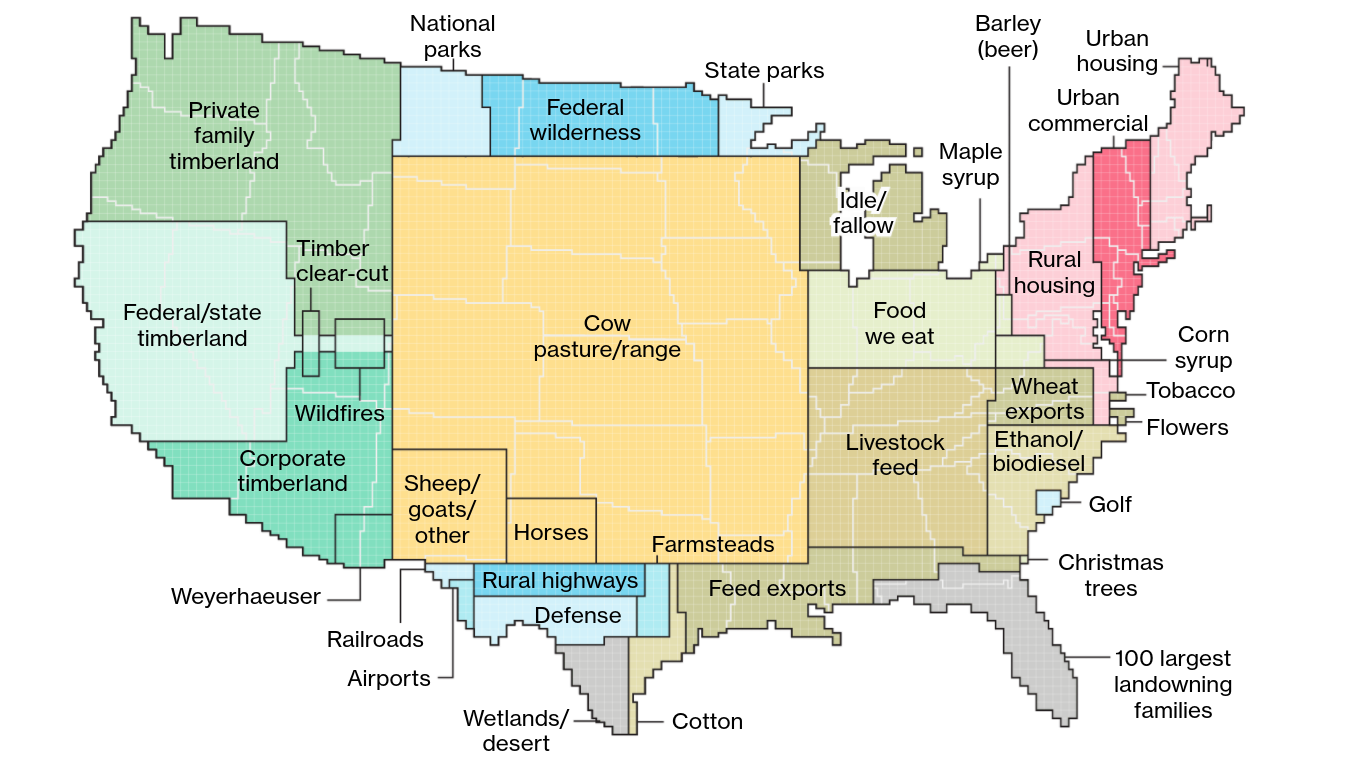
\includegraphics[keepaspectratio,
                                 width=\paperwidth]{images/how-america-uses-its-land.png}
            };
        \end{tikzpicture}
  \note[item]{90\% biomass on Earth is humans and livestock}
     \end{frame}
}




{ % all template changes are local to this group.
    \setbeamertemplate{navigation symbols}{}
    \begin{frame}<article:0>[plain]
      \frametitle{}
        \begin{tikzpicture}[remember picture,overlay]
            \node[at=(current page.center)] {
                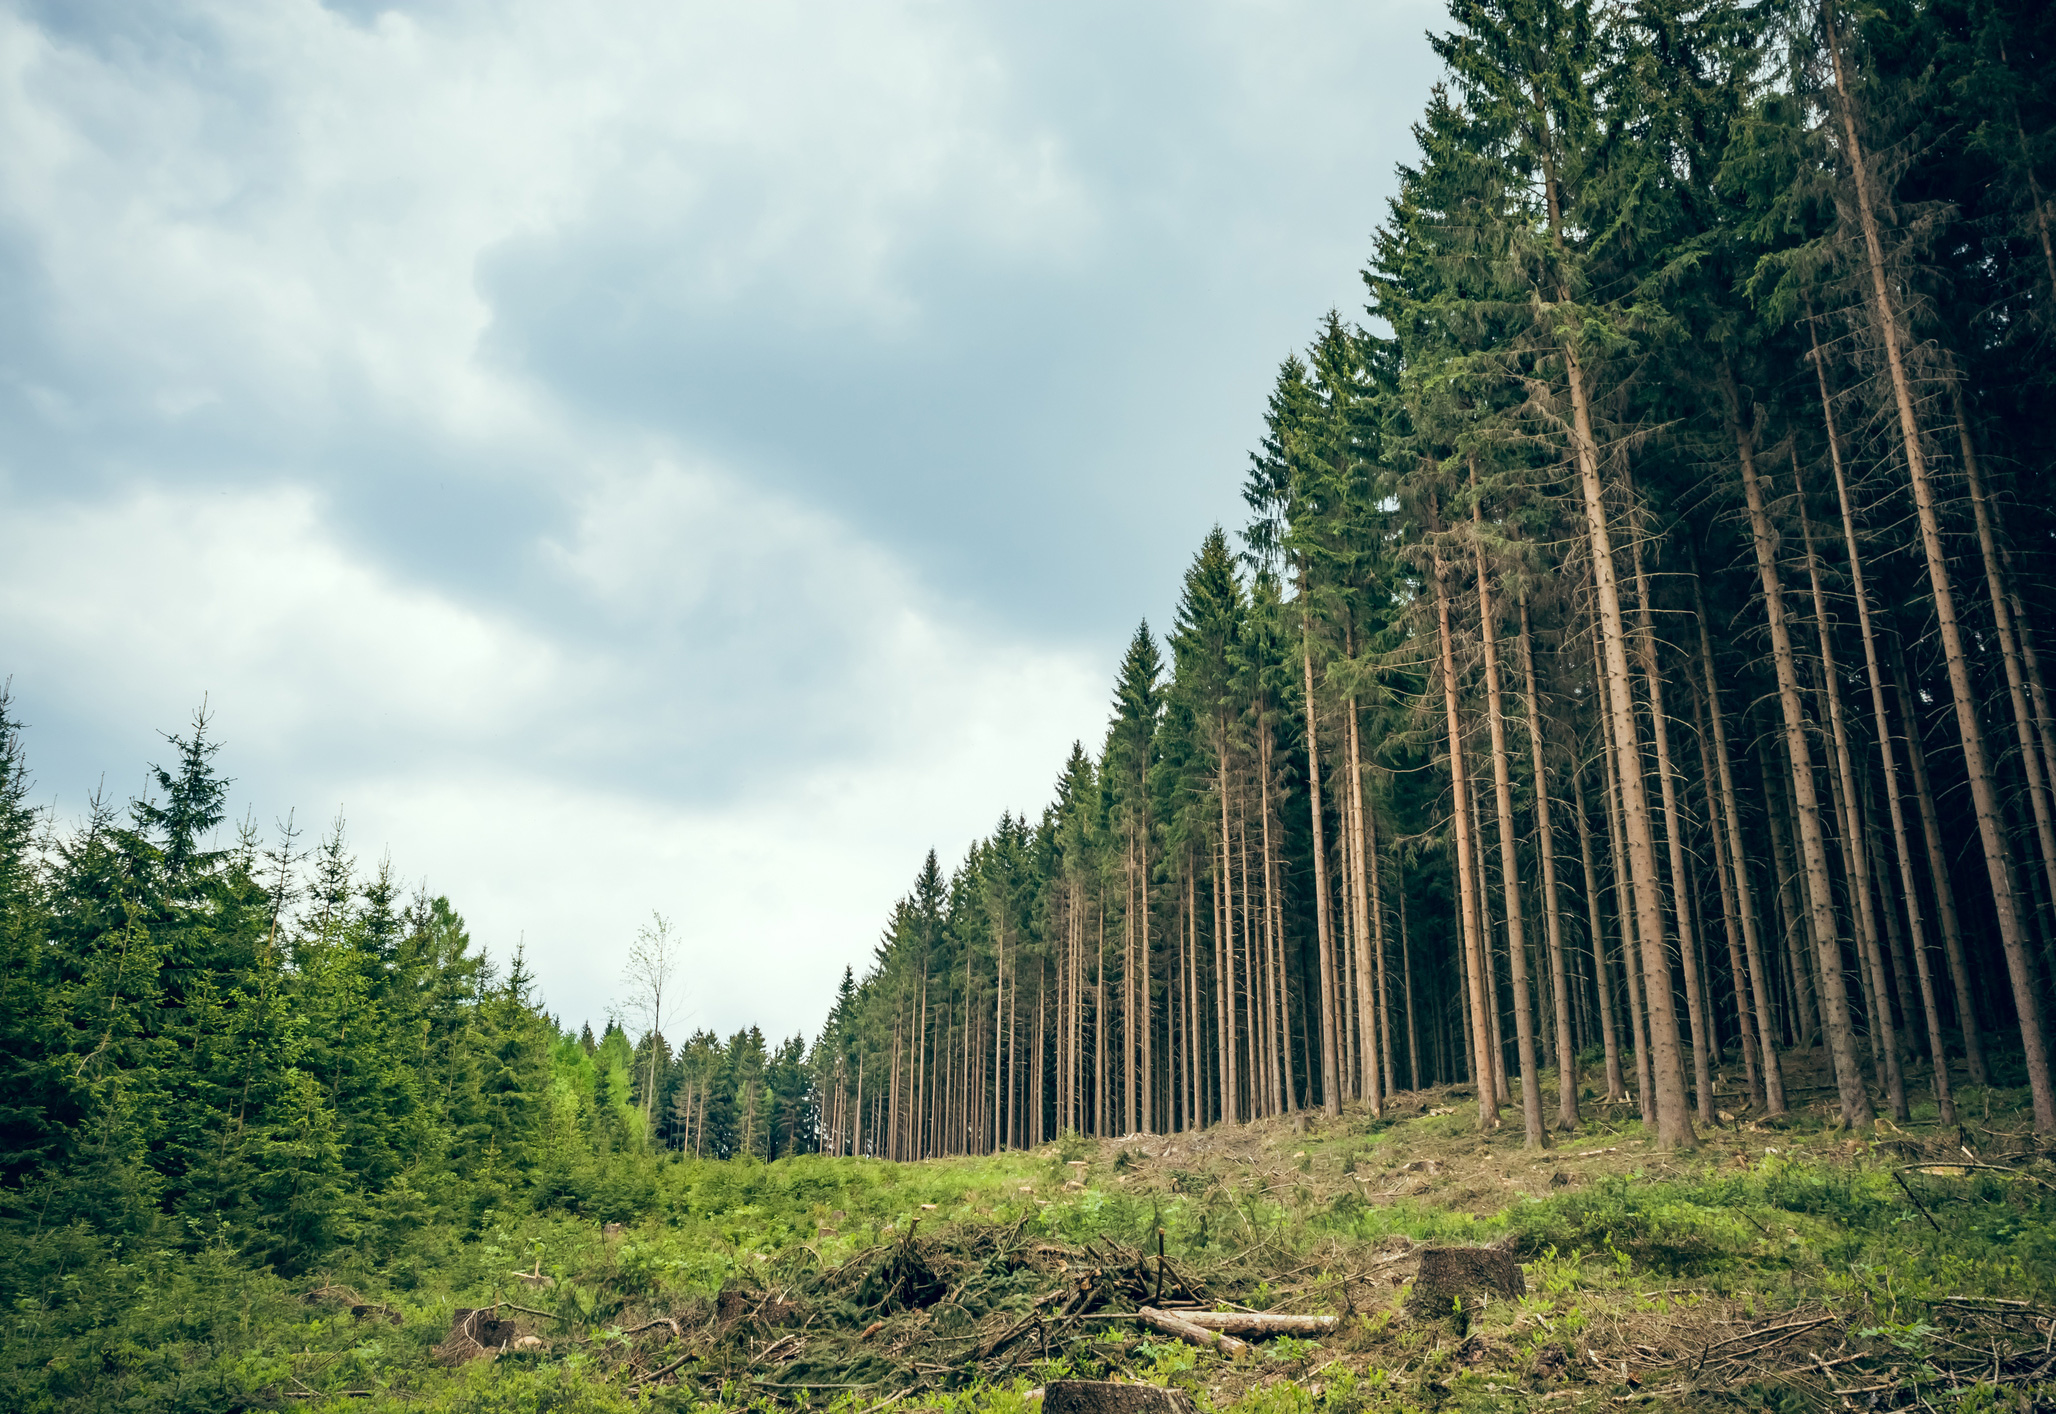
\includegraphics[keepaspectratio,
                                 width=\paperwidth]{images/forest-cut.jpg}
            };
        \end{tikzpicture}
     \end{frame}
}

{ % all template changes are local to this group.
    \setbeamertemplate{navigation symbols}{}
    \begin{frame}<article:0>[plain]
      \frametitle{}
        \begin{tikzpicture}[remember picture,overlay]
            \node[at=(current page.center)] {
                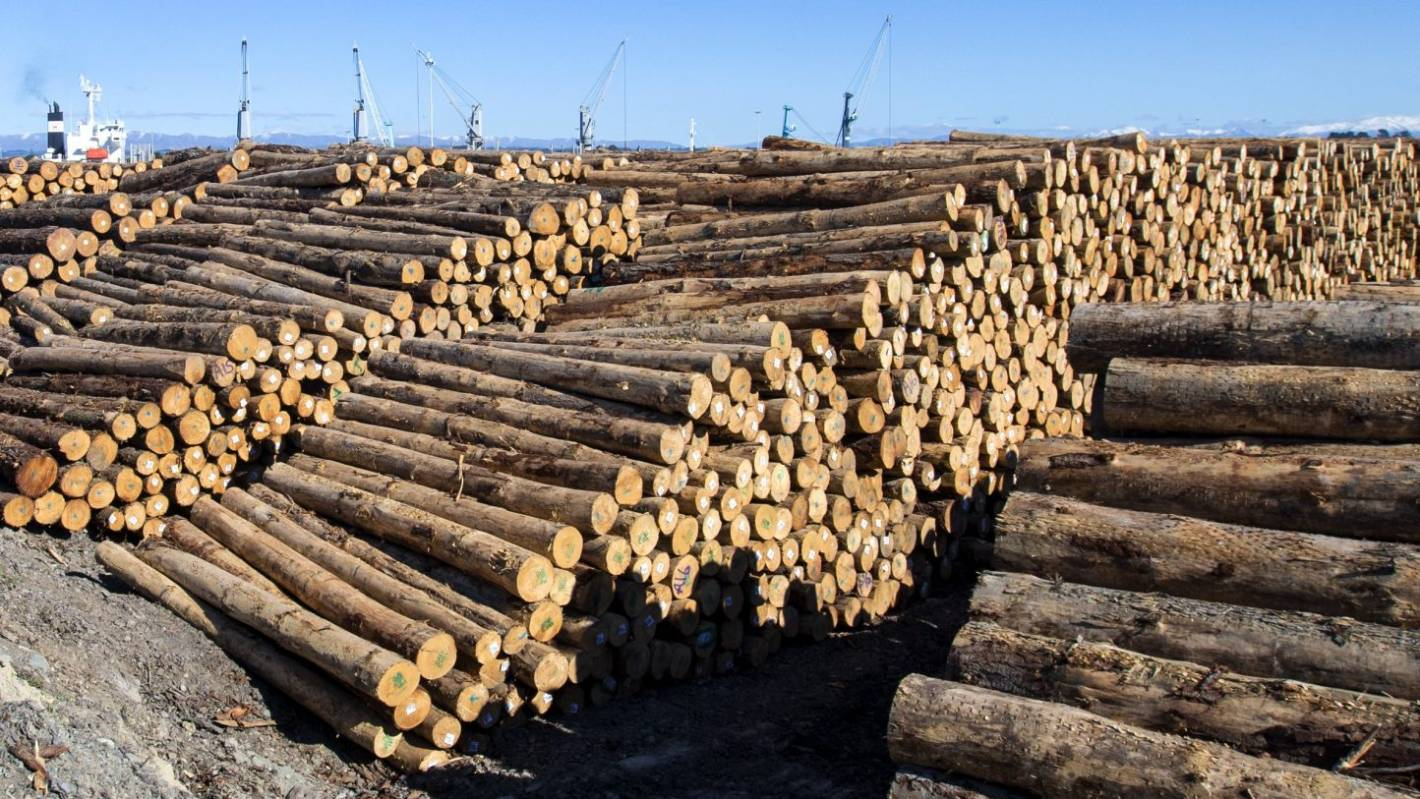
\includegraphics[keepaspectratio,
                                 width=\paperwidth]{images/sawn-logs.jpg}
            };
        \end{tikzpicture}
     \end{frame}
}






{ % all template changes are local to this group.
    \setbeamertemplate{navigation symbols}{}
    \begin{frame}<article:0>[plain]
      \frametitle{}
        \begin{tikzpicture}[remember picture,overlay]
            \node[at=(current page.center)] {
                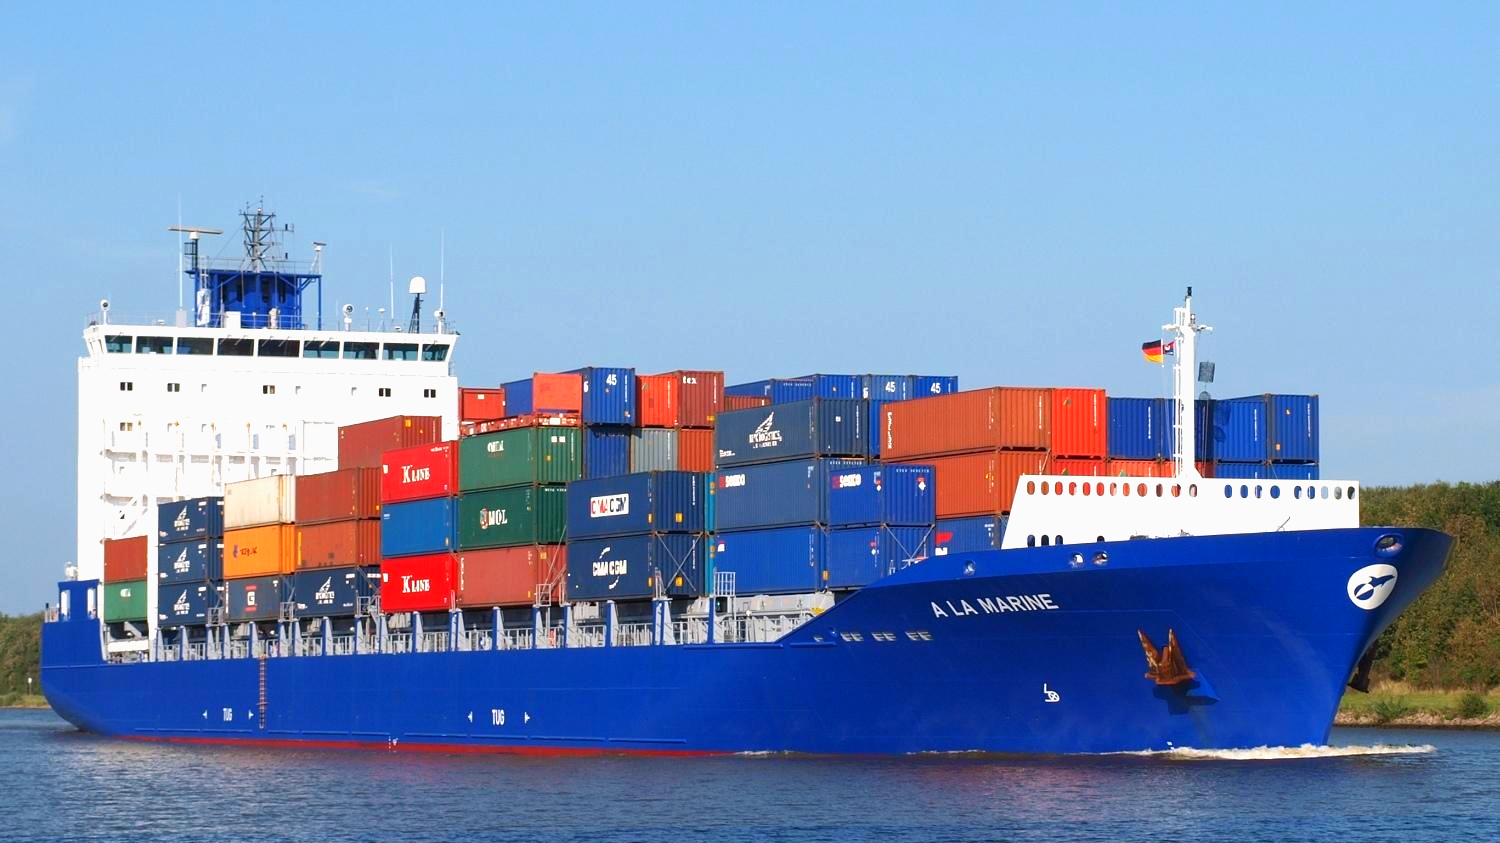
\includegraphics[keepaspectratio,
                                 width=\paperwidth]{images/shipping-ship.jpg}
            };
        \end{tikzpicture}
     \end{frame}
}


{ % all template changes are local to this group.
    \setbeamertemplate{navigation symbols}{}
    \begin{frame}<article:0>[plain]
      \frametitle{}
        \begin{tikzpicture}[remember picture,overlay]
            \node[at=(current page.center)] {
                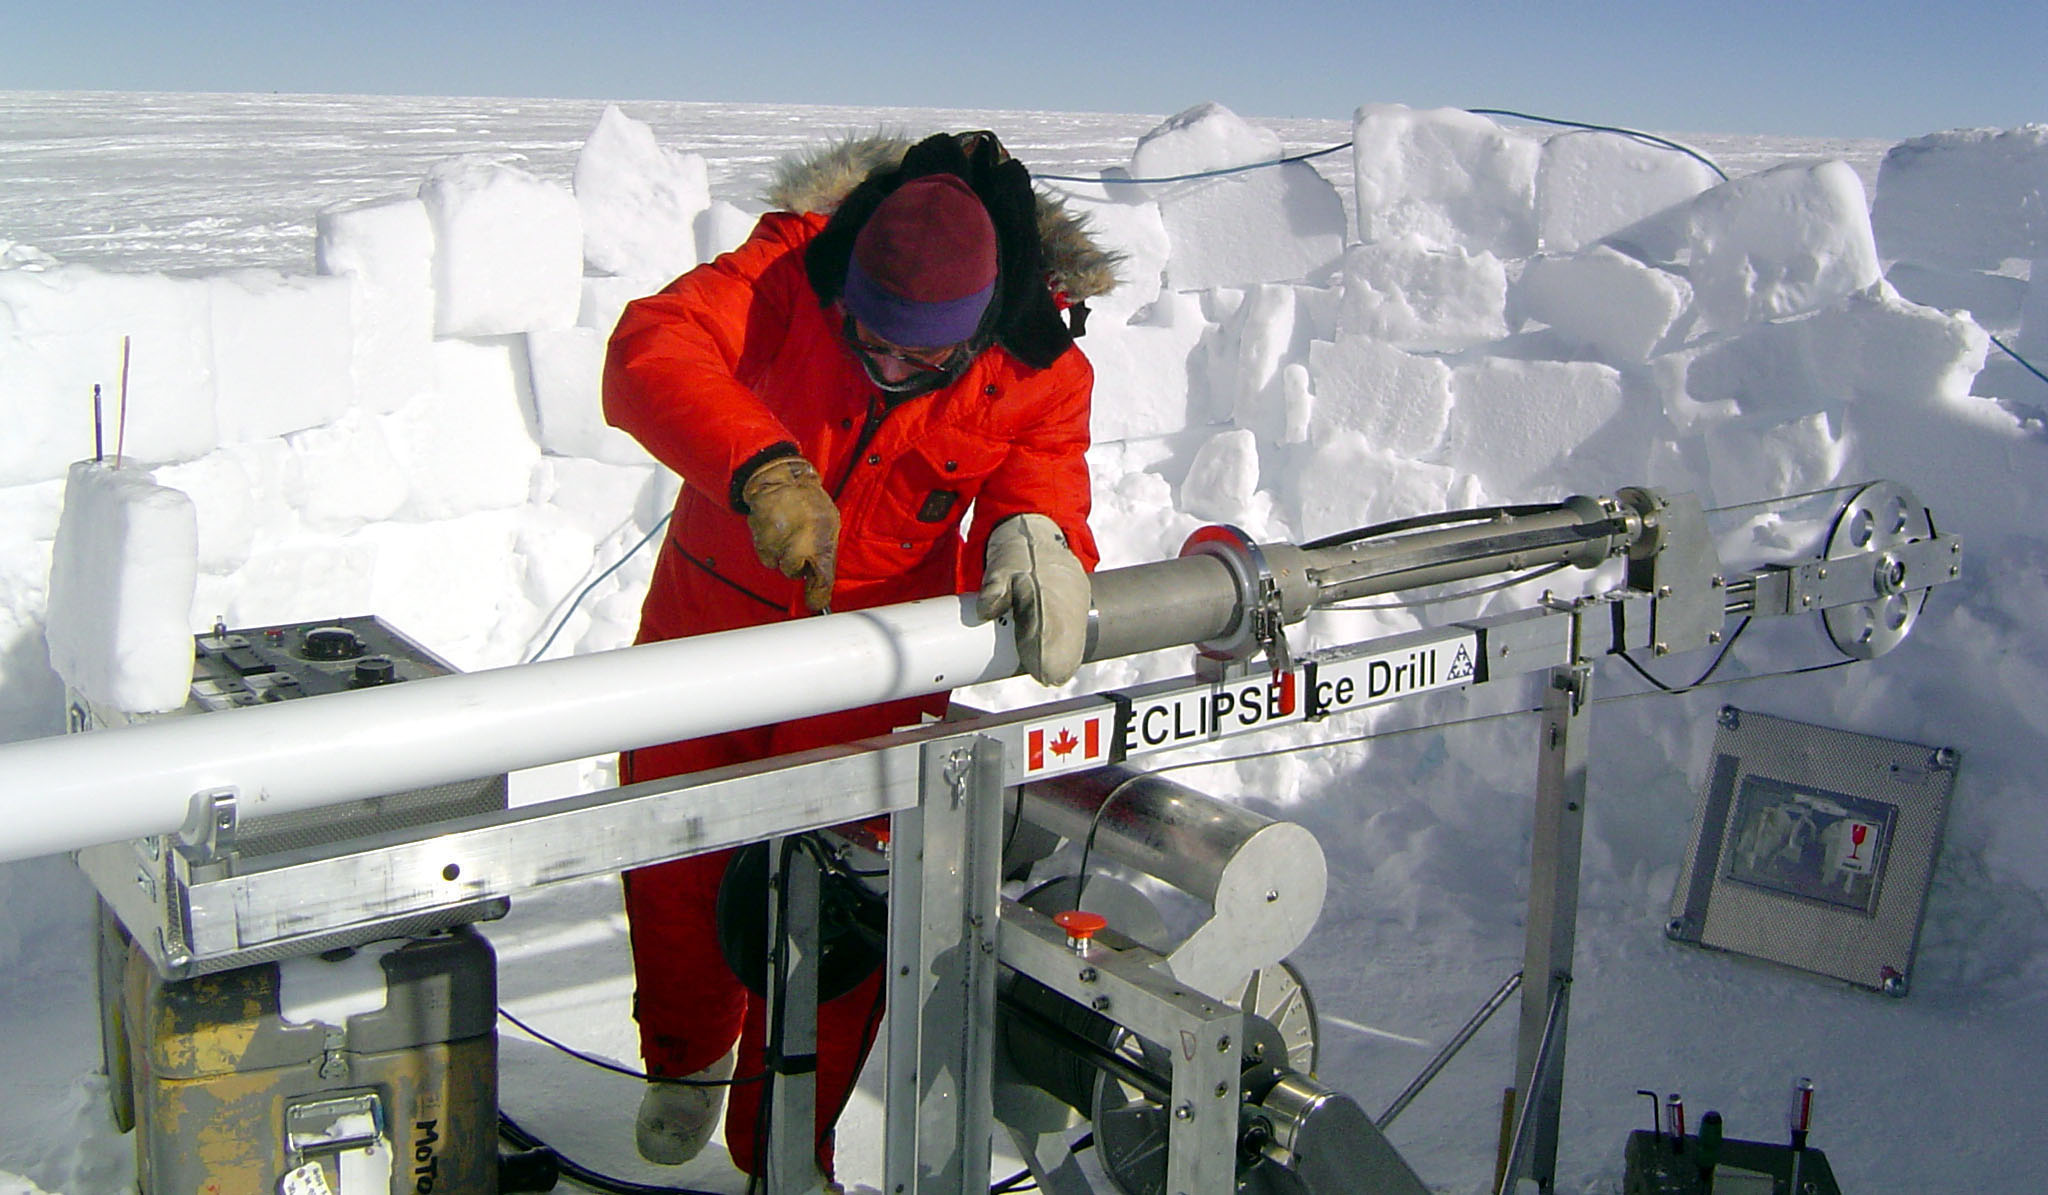
\includegraphics[keepaspectratio,
                                 width=\paperwidth]{images/ice_core.jpg}
            };
        \end{tikzpicture}
  \note[item]{Atmospheric changes = climate change, fire}
     \end{frame}
}

{ % all template changes are local to this group.
    \setbeamertemplate{navigation symbols}{}
    \begin{frame}<article:0>[plain]
      \frametitle{}
        \begin{tikzpicture}[remember picture,overlay]
            \node[at=(current page.center)] {
                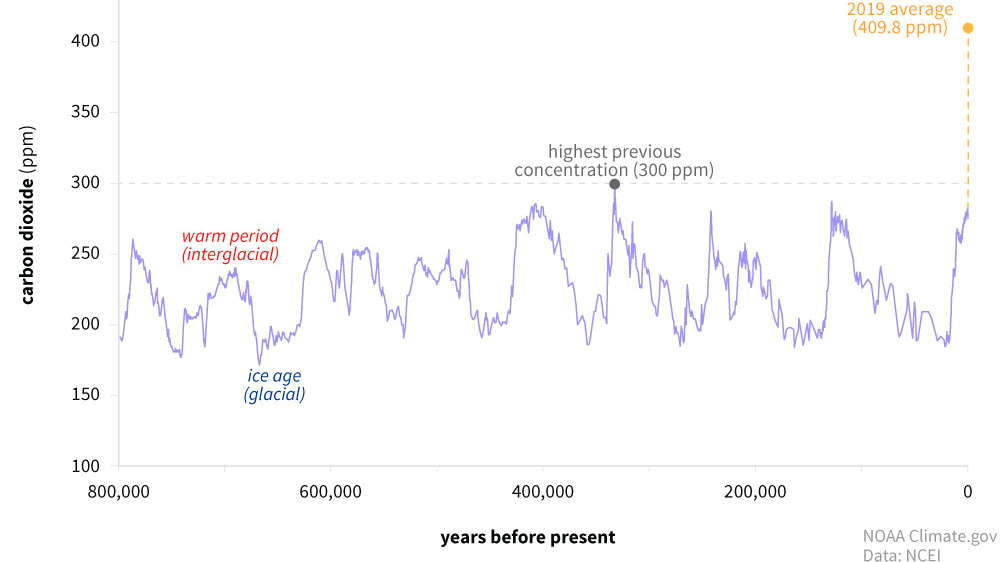
\includegraphics[keepaspectratio,
                                 width=\paperwidth]{images/BAMS_SOTC_2019_co2_paleo_1000px.jpg}
            };
        \end{tikzpicture}
     \end{frame}
}

{ % all template changes are local to this group.
    \setbeamertemplate{navigation symbols}{}
    \begin{frame}<article:0>[plain]
      \frametitle{}
        \begin{tikzpicture}[remember picture,overlay]
            \node[at=(current page.center)] {
                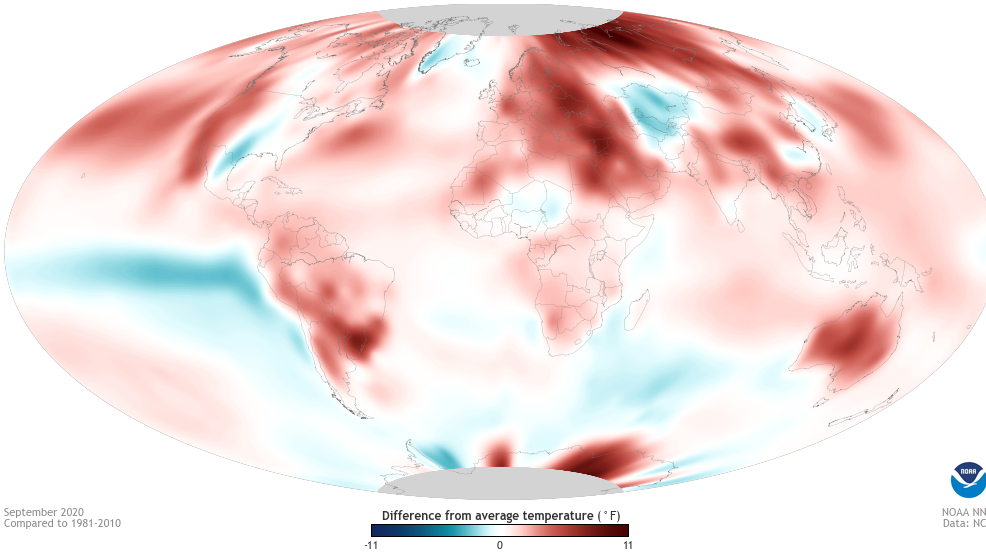
\includegraphics[keepaspectratio,
                                 width=\paperwidth]{images/September_CC2020.png}
            };
        \end{tikzpicture}
     \end{frame}
}

{ % all template changes are local to this group.
    \setbeamertemplate{navigation symbols}{}
    \begin{frame}<article:0>[plain]
      \frametitle{}
        \begin{tikzpicture}[remember picture,overlay]
            \node[at=(current page.center)] {
                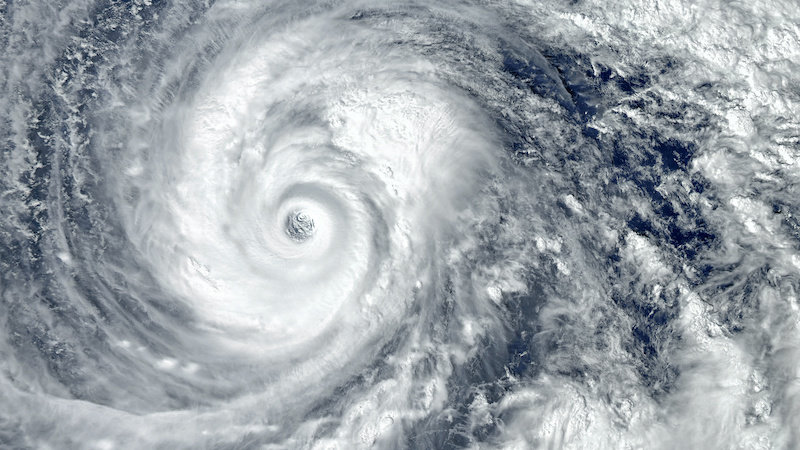
\includegraphics[keepaspectratio,
                                 width=\paperwidth]{images/hurricane.jpg}
            };
        \end{tikzpicture}
     \note[item]{Climate change is causing hurricanes that make
     landfall to take more time to weaken, reports a study published
     11th November 2020 in the journal Nature.}
     \end{frame}
}

{ % all template changes are local to this group.
    \setbeamertemplate{navigation symbols}{}
    \begin{frame}<article:0>[plain]
      \frametitle{}
        \begin{tikzpicture}[remember picture,overlay]
            \node[at=(current page.center)] {
                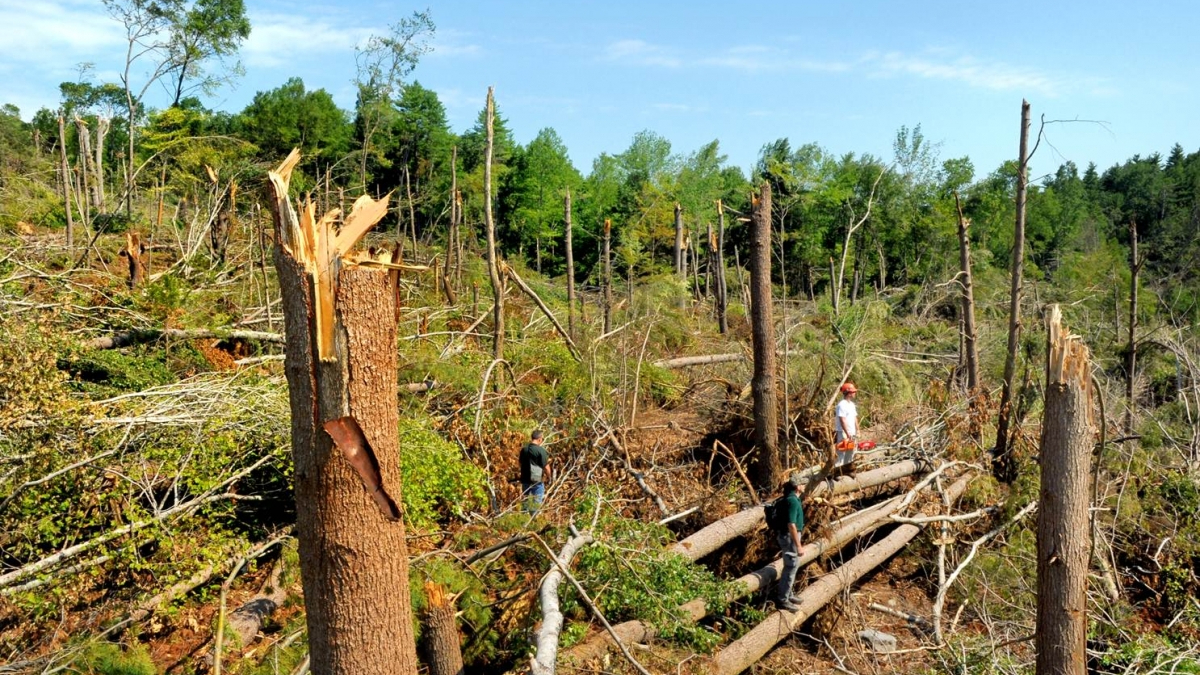
\includegraphics[keepaspectratio,
                                 width=\paperwidth]{images/tornado_hf.jpg}
            };
        \end{tikzpicture}
     \note[item]{Tornado damaged Southbridge, MA forest in 2011}
     \end{frame}
}



{ % all template changes are local to this group.
    \setbeamertemplate{navigation symbols}{}
    \begin{frame}<article:0>[plain]
      \frametitle{}
        \begin{tikzpicture}[remember picture,overlay]
            \node[at=(current page.center)] {
                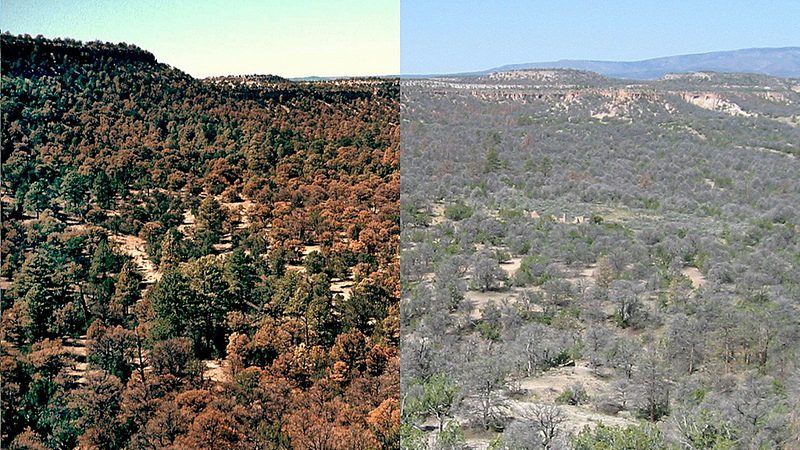
\includegraphics[keepaspectratio,
                                 width=\paperwidth]{images/drought_pjw.jpg}
            };
        \end{tikzpicture}
        \note[item]{Droughts}
     \end{frame}
}



{ % all template changes are local to this group.
    \setbeamertemplate{navigation symbols}{}
    \begin{frame}<article:0>[plain]
      \frametitle{}
        \begin{tikzpicture}[remember picture,overlay]
            \node[at=(current page.center)] {
                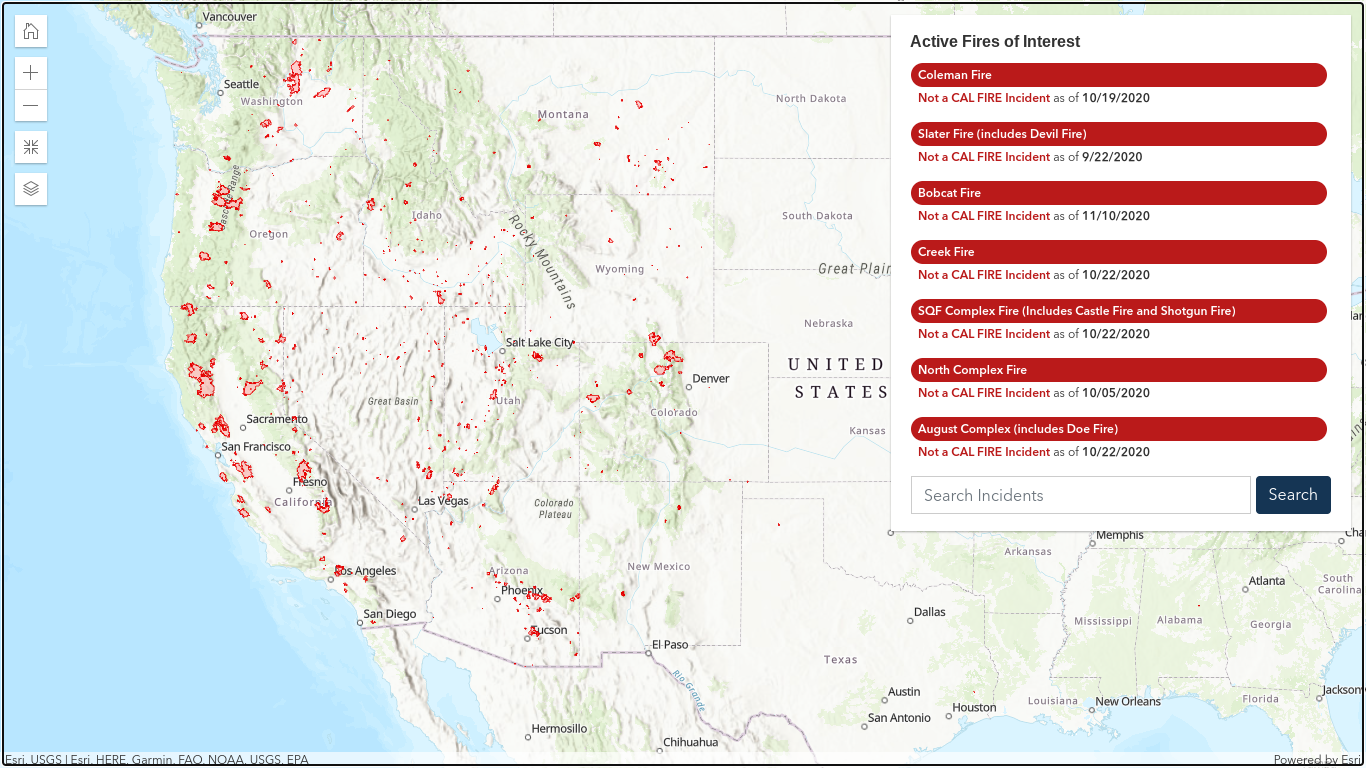
\includegraphics[keepaspectratio,
                                  width=\paperwidth]{images/fires_CALFIRE.png}
            };
        \end{tikzpicture}
        \note[item]{CAL FIRE MAP Tue 17 Nov 2020 12:10:52 PM EST}
     \end{frame}
}


{ % all template changes are local to this group.
    \setbeamertemplate{navigation symbols}{}
    \begin{frame}<article:0>[plain]
      \frametitle{}
        \begin{tikzpicture}[remember picture,overlay]
            \node[at=(current page.center)] {
                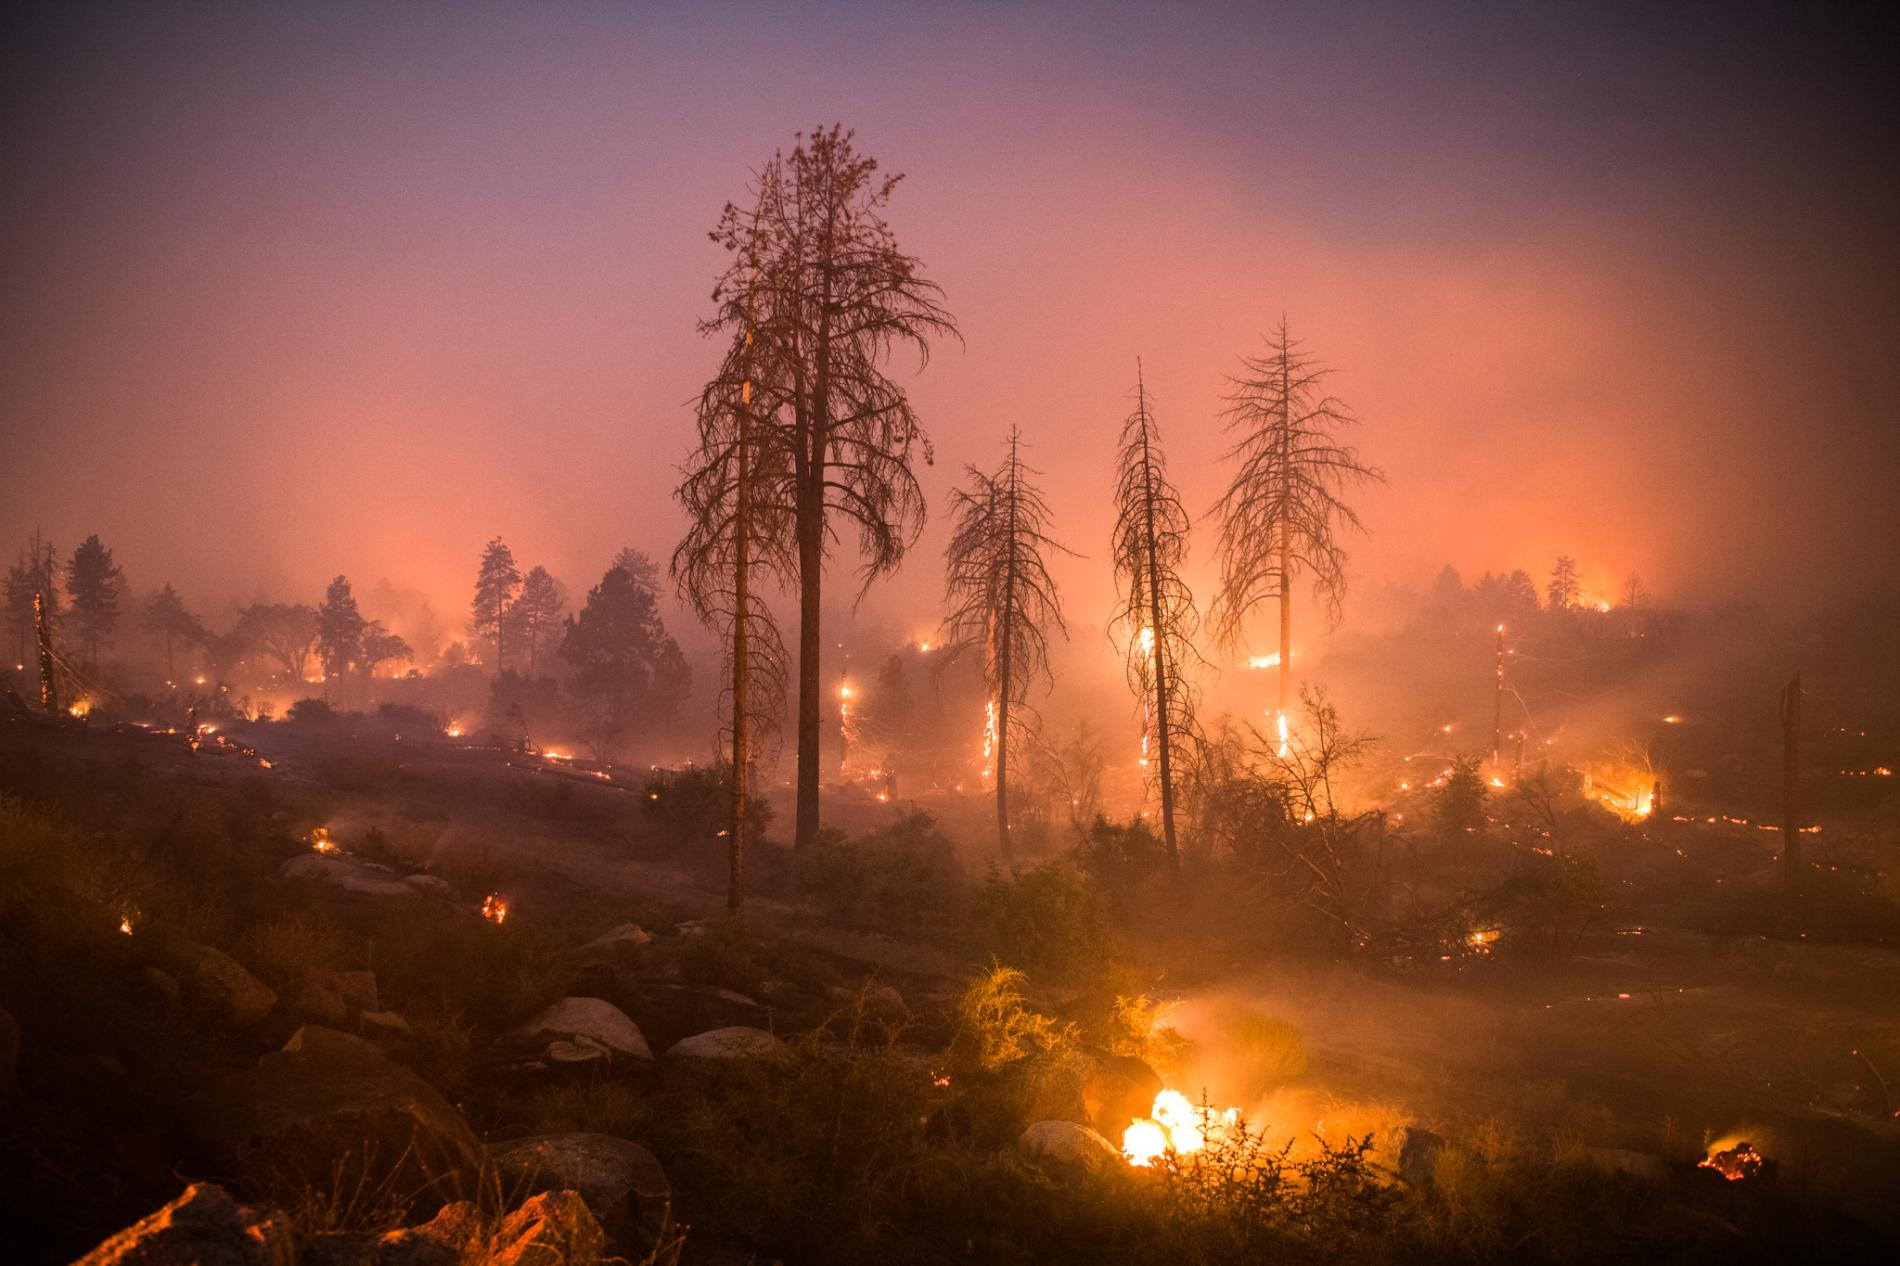
\includegraphics[keepaspectratio,
                                 width=\paperwidth]{images/fires_CAcranston.jpg}
            };
        \end{tikzpicture}
        \note[item]{CA Cranston Riverside 2018}
     \end{frame}
}


{ % all template changes are local to this group.
    \setbeamertemplate{navigation symbols}{}
    \begin{frame}<article:0>[plain]
      \frametitle{}
        \begin{tikzpicture}[remember picture,overlay]
            \node[at=(current page.center)] {
                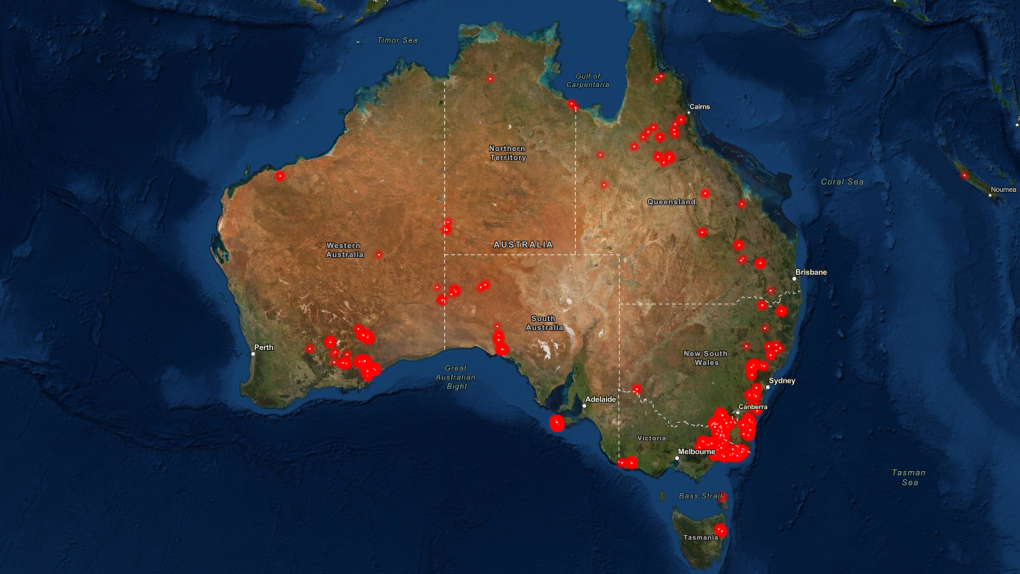
\includegraphics[keepaspectratio,
                                 width=\paperwidth]{images/fires_AUS.png}
            };
        \end{tikzpicture}
        \note[item]{Fires in Australia 2020}
     \end{frame}
}







\begin{frame}
  \frametitle{Forests in the Anthropocence}
  
  \begin{itemize}
  \item Forests are changing from human impacts \pause
  \item Large direct and \underline{indirect} effects of land-use  \pause
  \item How do we address indirect and systems-level effects? 
  \end{itemize}

\end{frame}


\begin{frame}
  \frametitle{Today's Talk}

\tableofcontents

\note[item]{Intro/Context}
\note[item]{Global forest loss and gain and change}
\note[item]{Global greening = India(Agriculture) + China(Forests)}
\note[item]{Economics*Ecology = Landscape Extended Models}
\note[item]{Network Analysis of China's Greening}
\note[item]{Global Scale}
\note[item]{Local Scale}
\note[item]{Landscape = Tian 2019, Chen 2019}
\note[item]{Resilience Analysis of China's Forest LE-MRIO}
\note[item]{Conclusions and Future Work}
\note[item]{Acknowledgements}

\end{frame}





\section{Economic and Ecological Landscape Extensions}


{ % all template changes are local to this group.
    \setbeamertemplate{navigation symbols}{}
    \begin{frame}<article:0>[plain]
      \frametitle{}
        \begin{tikzpicture}[remember picture,overlay]
            \node[at=(current page.center)] {
                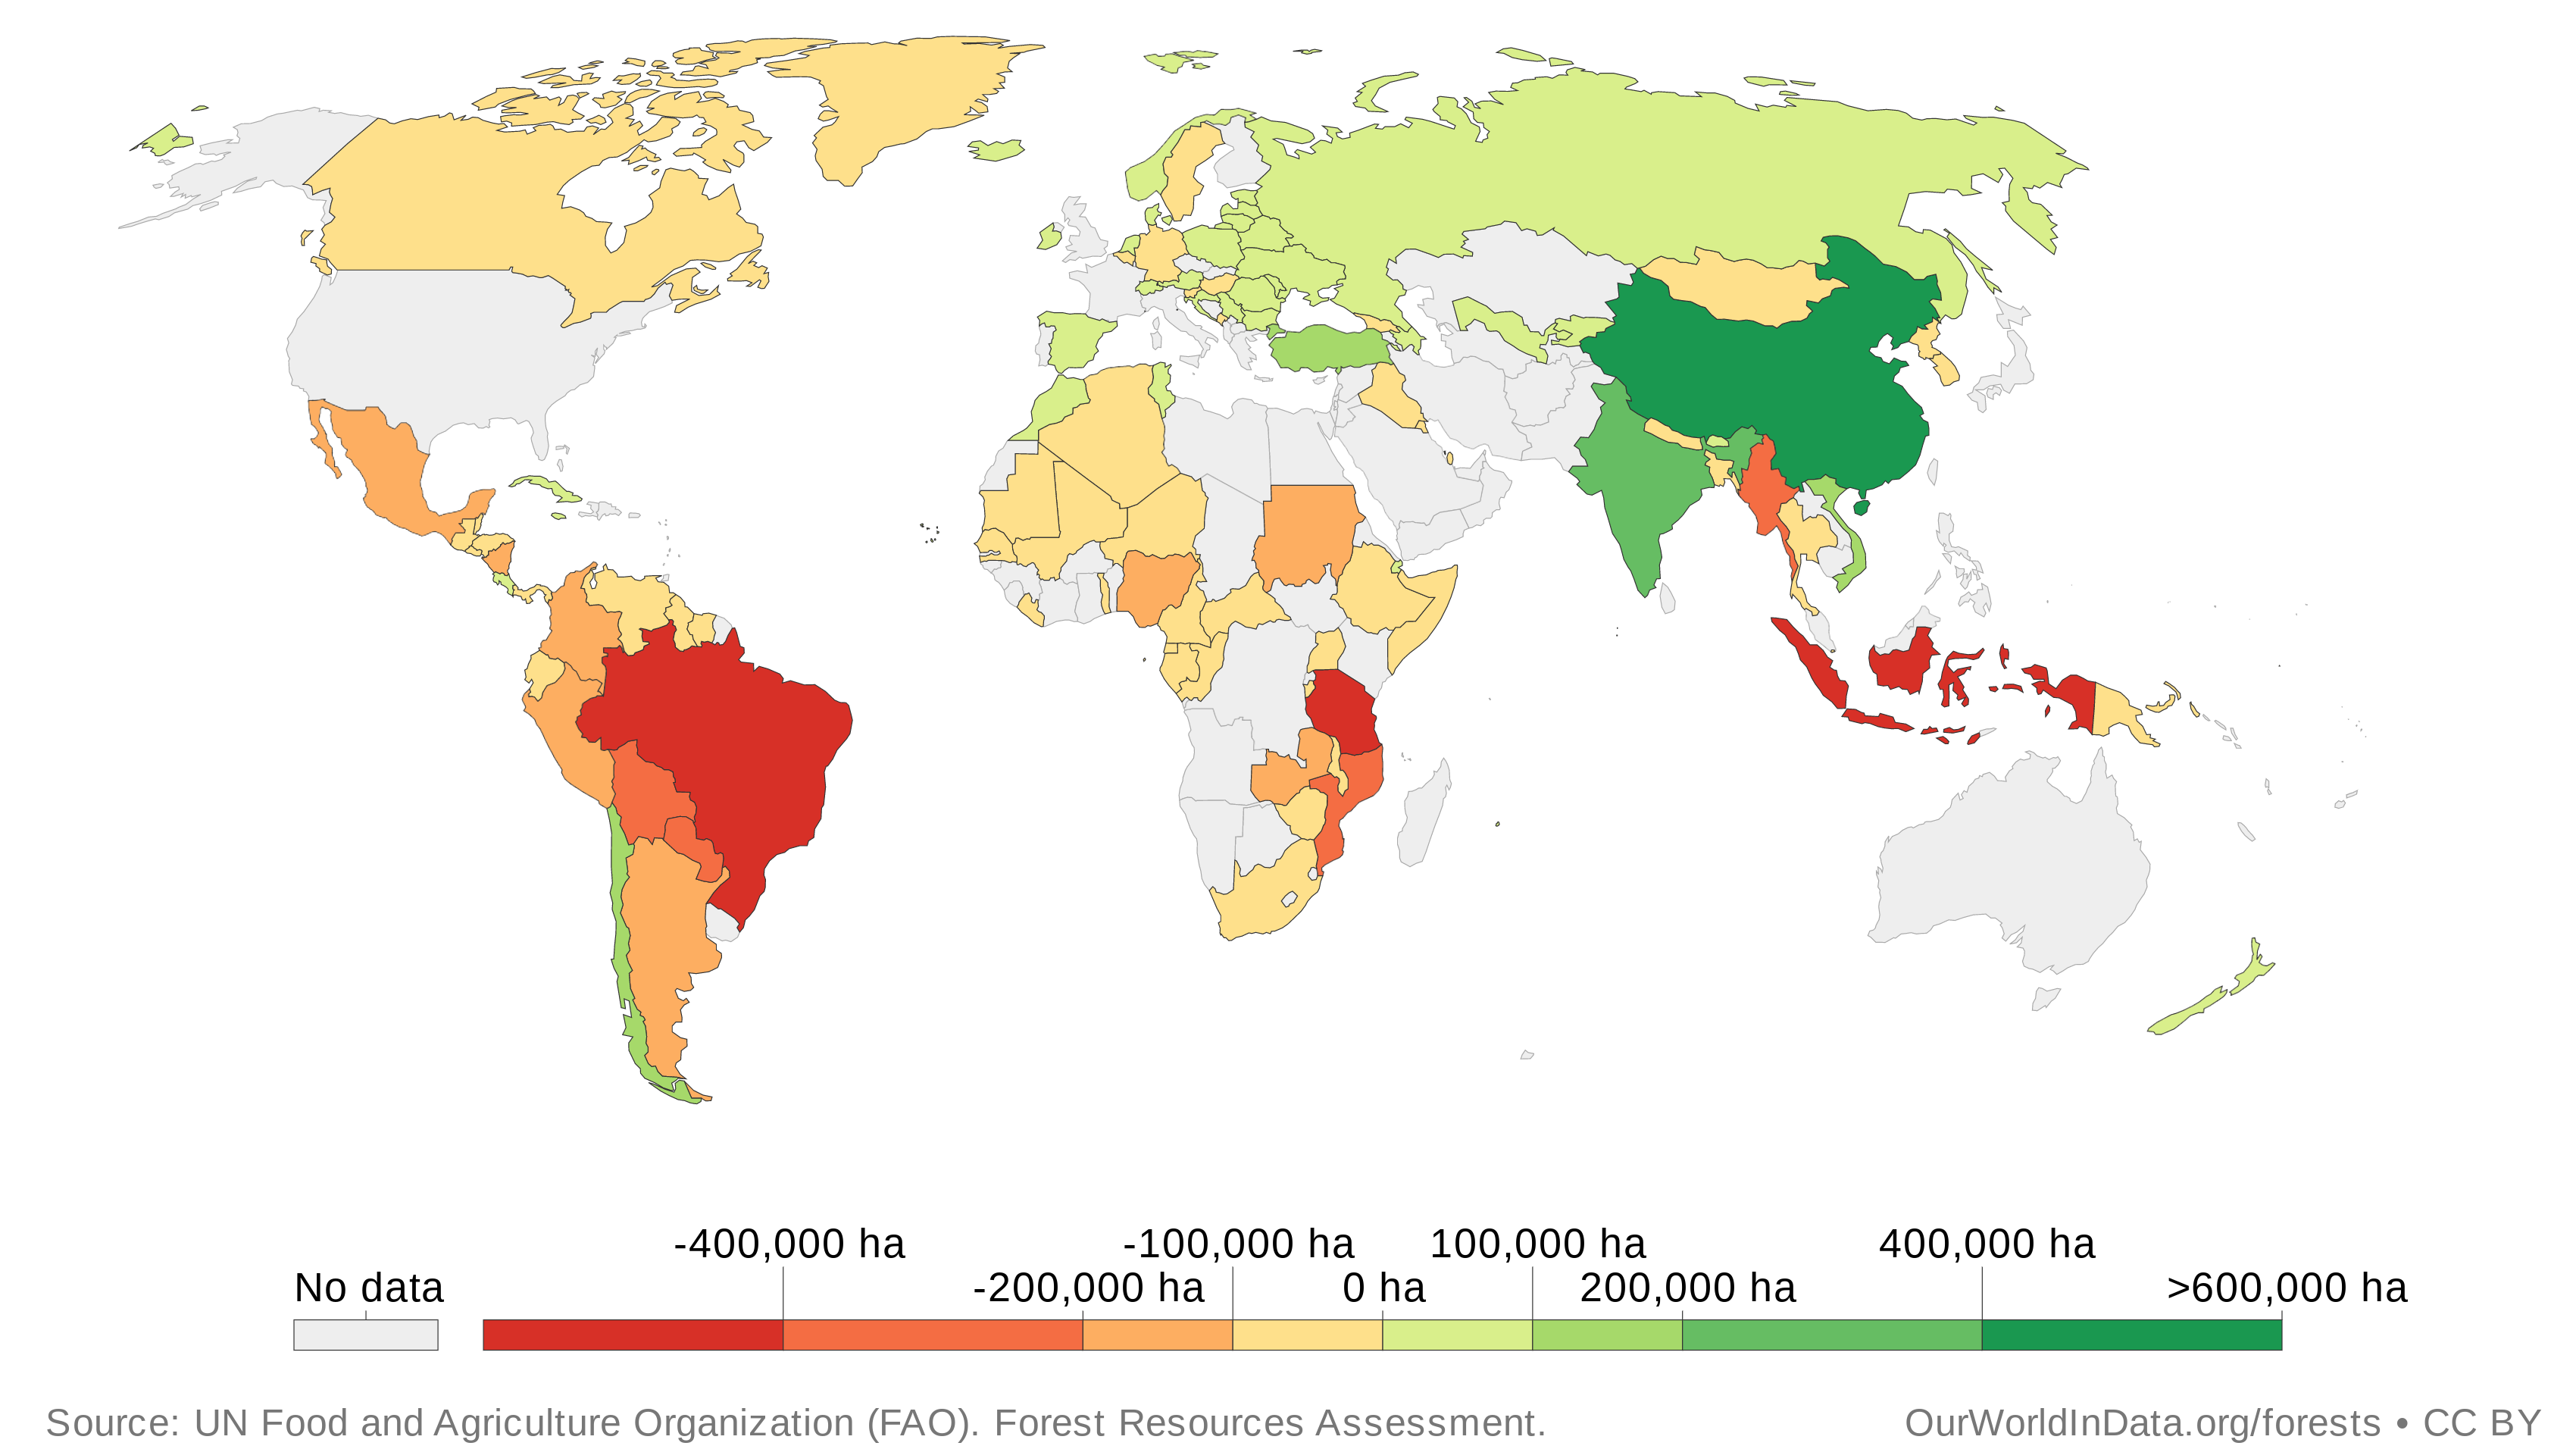
\includegraphics[keepaspectratio,
                                 width=\paperwidth]{images/annual-change-forest-area.png}
            };
        \end{tikzpicture}
        \note[item]{Global forest loss and gain and change}
        \note[item]{Global greening = India(Agriculture) + China(Forests)}
     \end{frame}
}



\begin{frame}
  \frametitle{Economic and Ecological Landscape Extensions}
\end{frame}


\section{Trade Networks of Forest Landscapes}

\begin{frame}
  \frametitle{Trade Networks of Forest Landscapes}
\end{frame}



\section{Global Forest Networks}

\begin{frame}
  \frametitle{Global Forest Networks}
\end{frame}


\section{China's Forest Networks}

{ % all template changes are local to this group.
    \setbeamertemplate{navigation symbols}{}
    \begin{frame}<article:0>[plain]
      \frametitle{}
        \begin{tikzpicture}[remember picture,overlay]
            \node[at=(current page.center)] {
                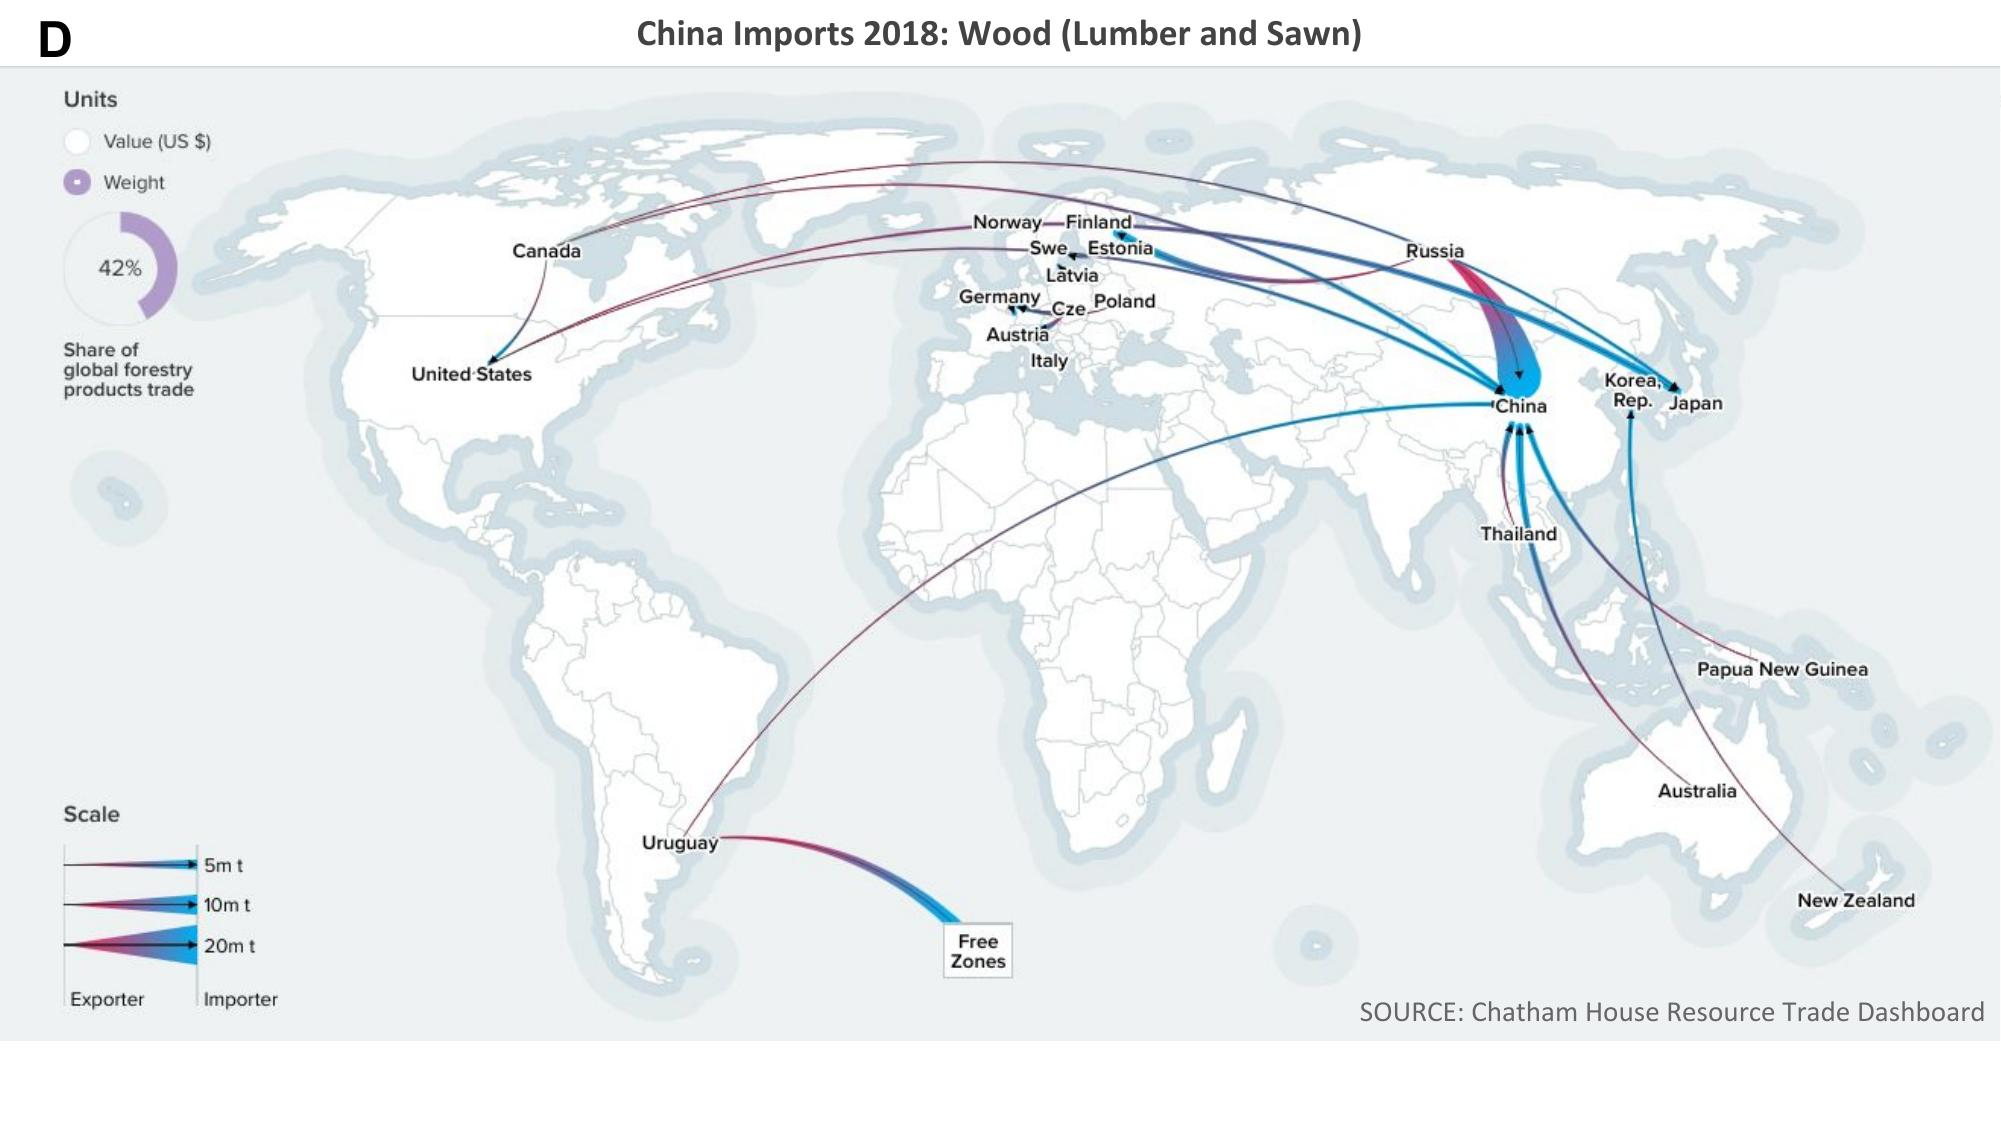
\includegraphics[keepaspectratio,
                                 width=\paperwidth]{images/resourcetrade_network.jpeg}
            };
        \end{tikzpicture}
     \end{frame}
}


{ % all template changes are local to this group.
    \setbeamertemplate{navigation symbols}{}
    \begin{frame}<article:0>[plain]
      \frametitle{}
        \begin{tikzpicture}[remember picture,overlay]
            \node[at=(current page.center)] {
                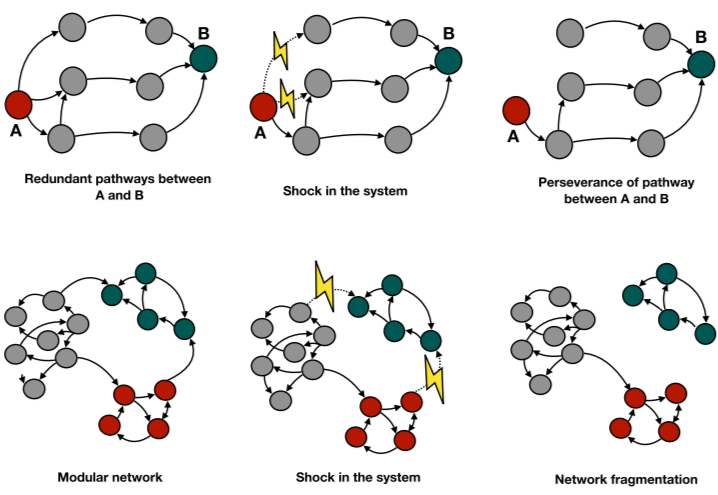
\includegraphics[keepaspectratio,
                                 width=\paperwidth]{images/net_info_dynamics.PNG}
            };
        \end{tikzpicture}
        \note[item]{China's Forests are Diverse}
     \end{frame}
}



{ % all template changes are local to this group.
    \setbeamertemplate{navigation symbols}{}
    \begin{frame}<article:0>[plain]
      \frametitle{}
        \begin{tikzpicture}[remember picture,overlay]
            \node[at=(current page.center)] {
                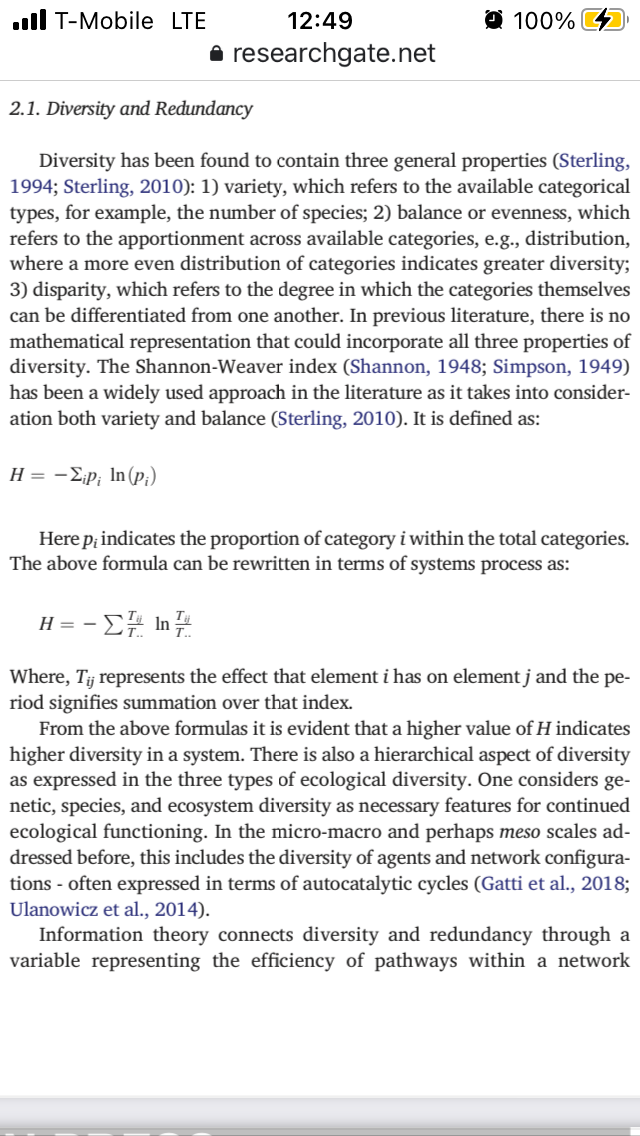
\includegraphics[keepaspectratio,
                                 width=\paperwidth]{images/cn_for_yu/IMG_0226.PNG}
            };
        \end{tikzpicture}
        \note[item]{China's Forests are Diverse}
     \end{frame}
}



{ % all template changes are local to this group.
    \setbeamertemplate{navigation symbols}{}
    \begin{frame}<article:0>[plain]
      \frametitle{}
        \begin{tikzpicture}[remember picture,overlay]
            \node[at=(current page.center)] {
                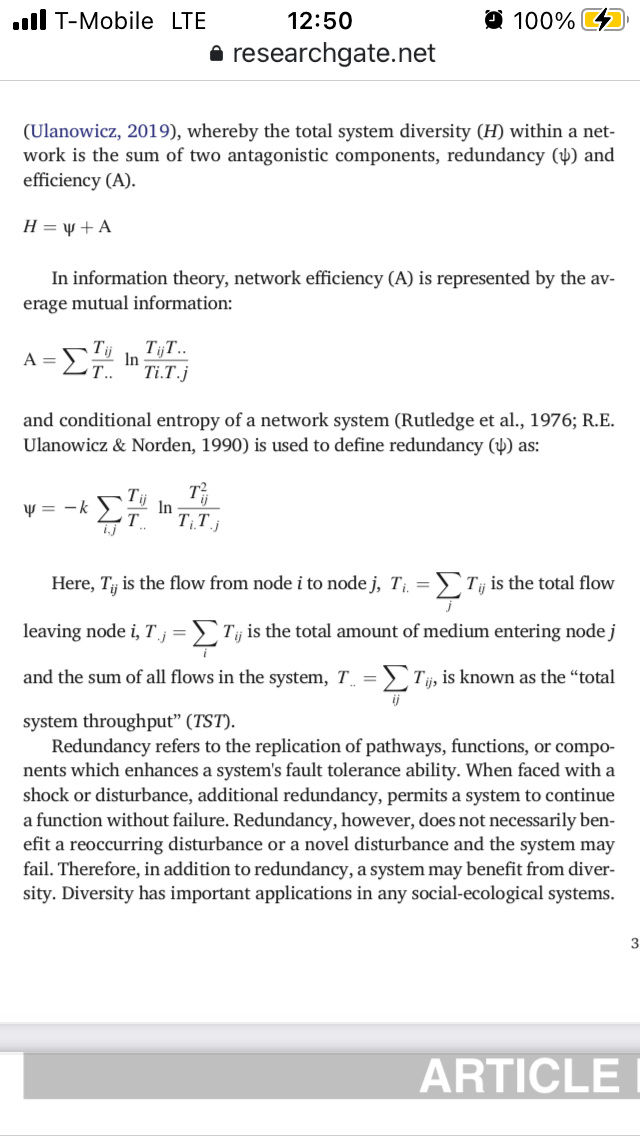
\includegraphics[keepaspectratio,
                                 width=\paperwidth]{images/cn_for_yu/IMG_0227.PNG}
            };
        \end{tikzpicture}
        \note[item]{China's Forests are Diverse}
     \end{frame}
}



{ % all template changes are local to this group.
    \setbeamertemplate{navigation symbols}{}
    \begin{frame}<article:0>[plain]
      \frametitle{}
        \begin{tikzpicture}[remember picture,overlay]
            \node[at=(current page.center)] {
                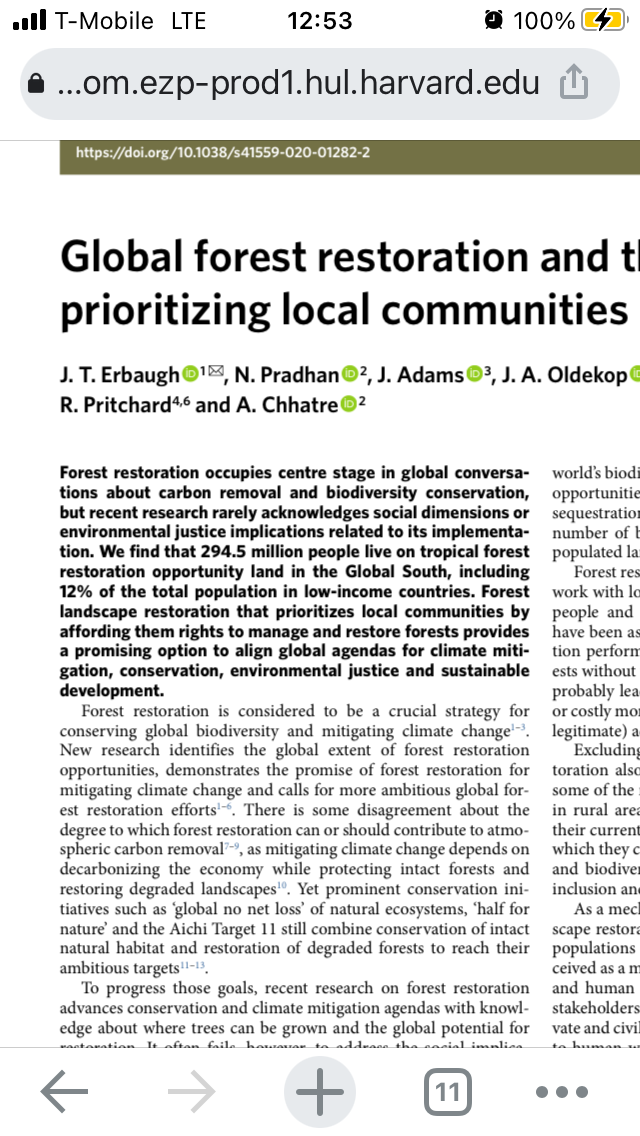
\includegraphics[keepaspectratio,
                                 width=\paperwidth]{images/cn_for_yu/IMG_0228.PNG}
            };
        \end{tikzpicture}
        \note[item]{China's Forests are Diverse}
     \end{frame}
}



{ % all template changes are local to this group.
    \setbeamertemplate{navigation symbols}{}
    \begin{frame}<article:0>[plain]
      \frametitle{}
        \begin{tikzpicture}[remember picture,overlay]
            \node[at=(current page.center)] {
                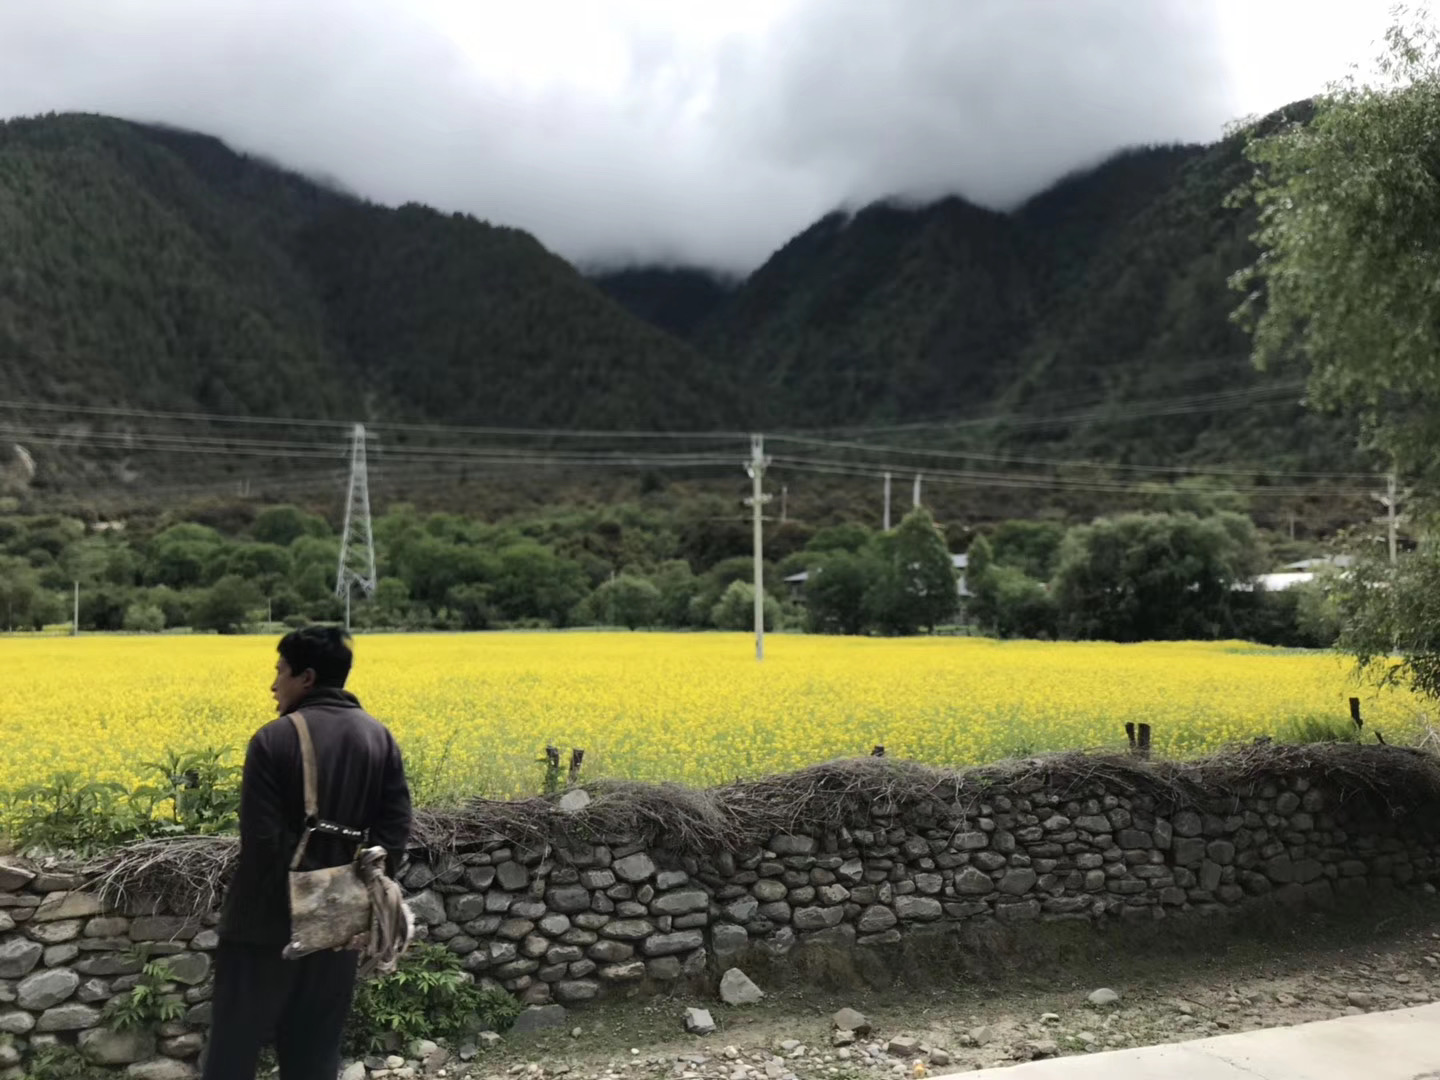
\includegraphics[keepaspectratio,
                                 width=\paperwidth]{images/cn_for_yu/IMG_0231.JPG}
            };
        \end{tikzpicture}
        \note[item]{China's Forests are Diverse}
     \end{frame}
}



{ % all template changes are local to this group.
    \setbeamertemplate{navigation symbols}{}
    \begin{frame}<article:0>[plain]
      \frametitle{}
        \begin{tikzpicture}[remember picture,overlay]
            \node[at=(current page.center)] {
                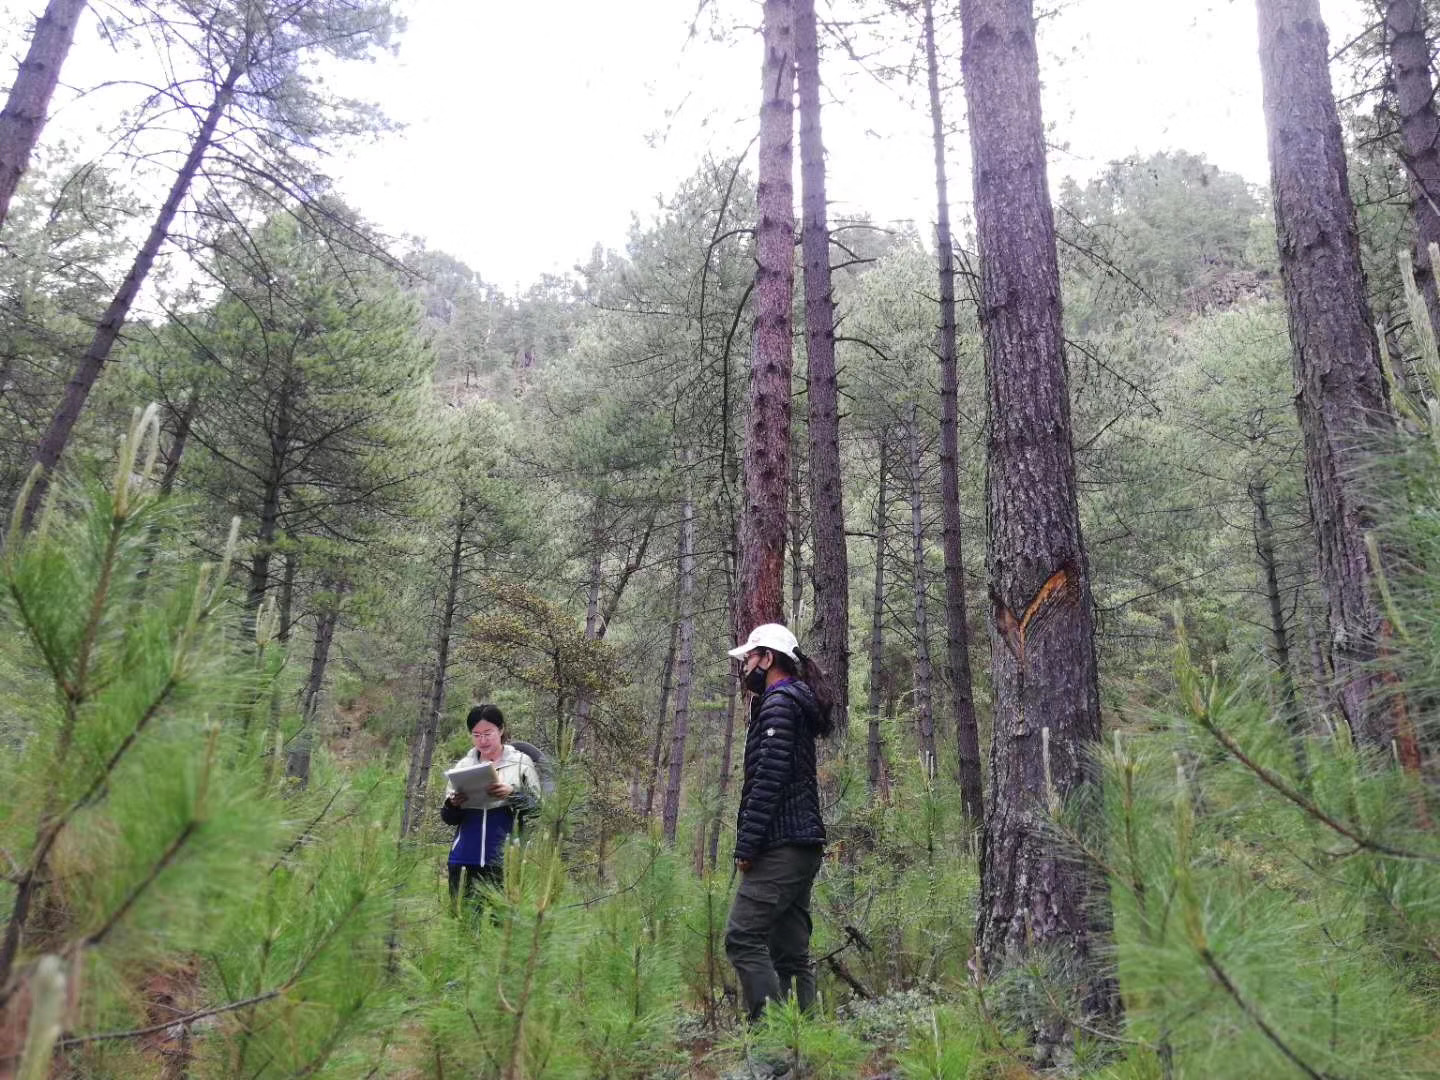
\includegraphics[keepaspectratio,
                                 width=\paperwidth]{images/cn_for_yu/IMG_0232.JPG}
            };
        \end{tikzpicture}
        \note[item]{China's Forests are Diverse}
     \end{frame}
}



{ % all template changes are local to this group.
    \setbeamertemplate{navigation symbols}{}
    \begin{frame}<article:0>[plain]
      \frametitle{}
        \begin{tikzpicture}[remember picture,overlay]
            \node[at=(current page.center)] {
                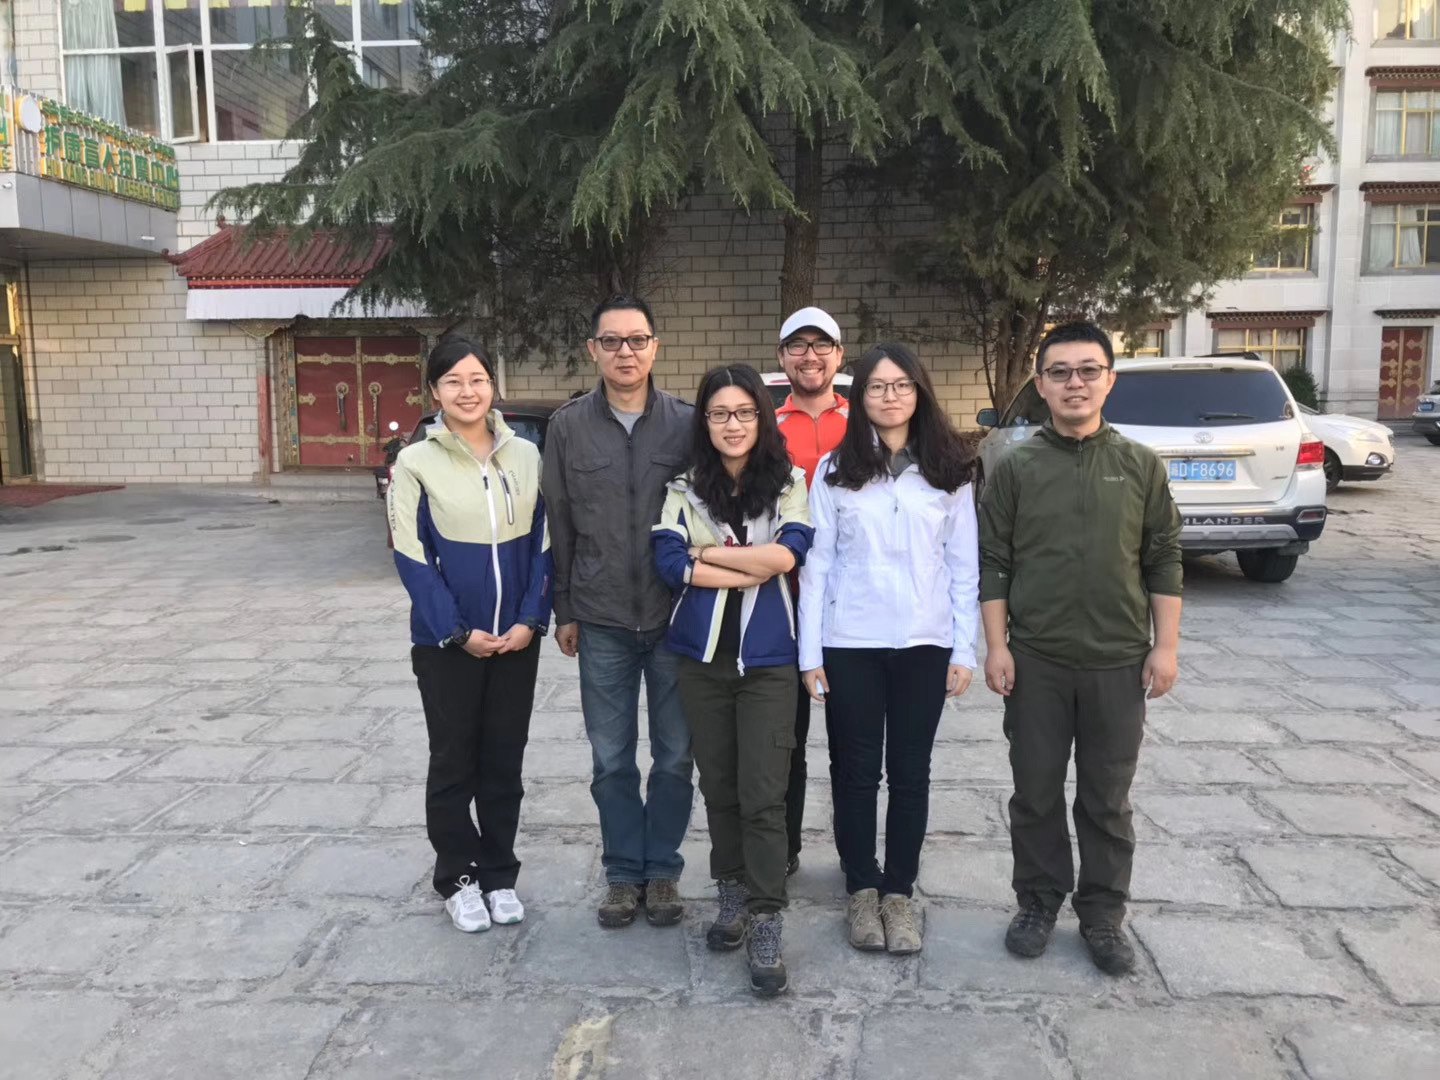
\includegraphics[keepaspectratio,
                                 width=\paperwidth]{images/cn_for_yu/IMG_0233.JPG}
            };
        \end{tikzpicture}
        \note[item]{China's Forests are Diverse}
     \end{frame}
}



{ % all template changes are local to this group.
    \setbeamertemplate{navigation symbols}{}
    \begin{frame}<article:0>[plain]
      \frametitle{}
        \begin{tikzpicture}[remember picture,overlay]
            \node[at=(current page.center)] {
                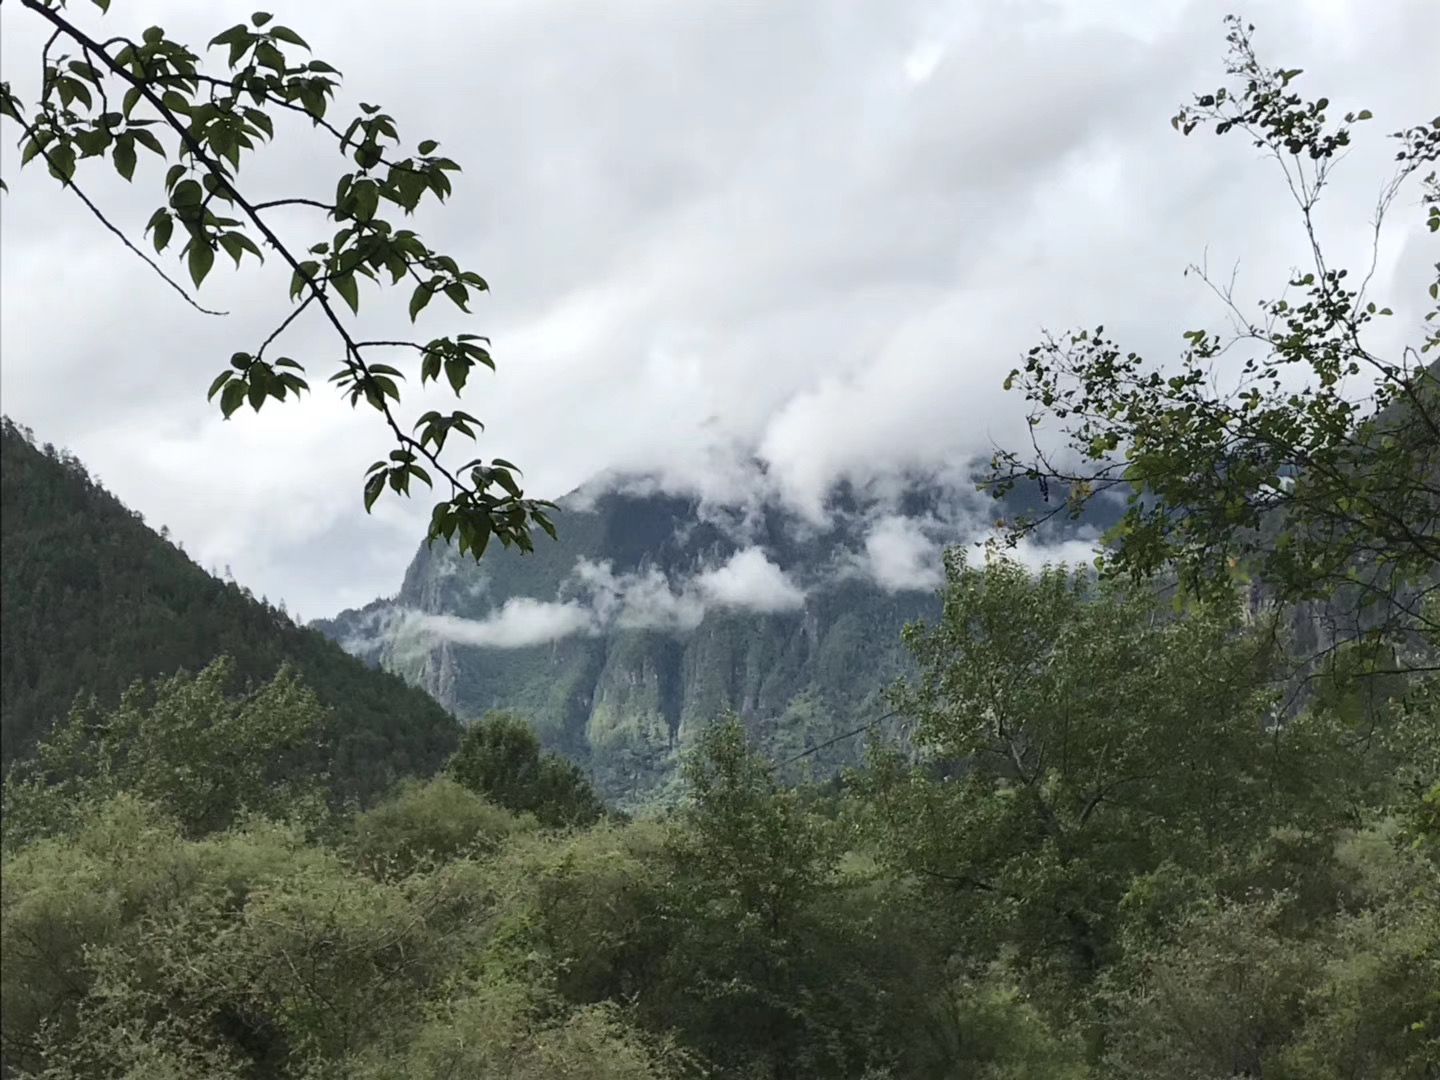
\includegraphics[keepaspectratio,
                                 width=\paperwidth]{images/cn_for_yu/IMG_0234.JPG}
            };
        \end{tikzpicture}
        \note[item]{China's Forests are Diverse}
     \end{frame}
}



{ % all template changes are local to this group.
    \setbeamertemplate{navigation symbols}{}
    \begin{frame}<article:0>[plain]
      \frametitle{}
        \begin{tikzpicture}[remember picture,overlay]
            \node[at=(current page.center)] {
                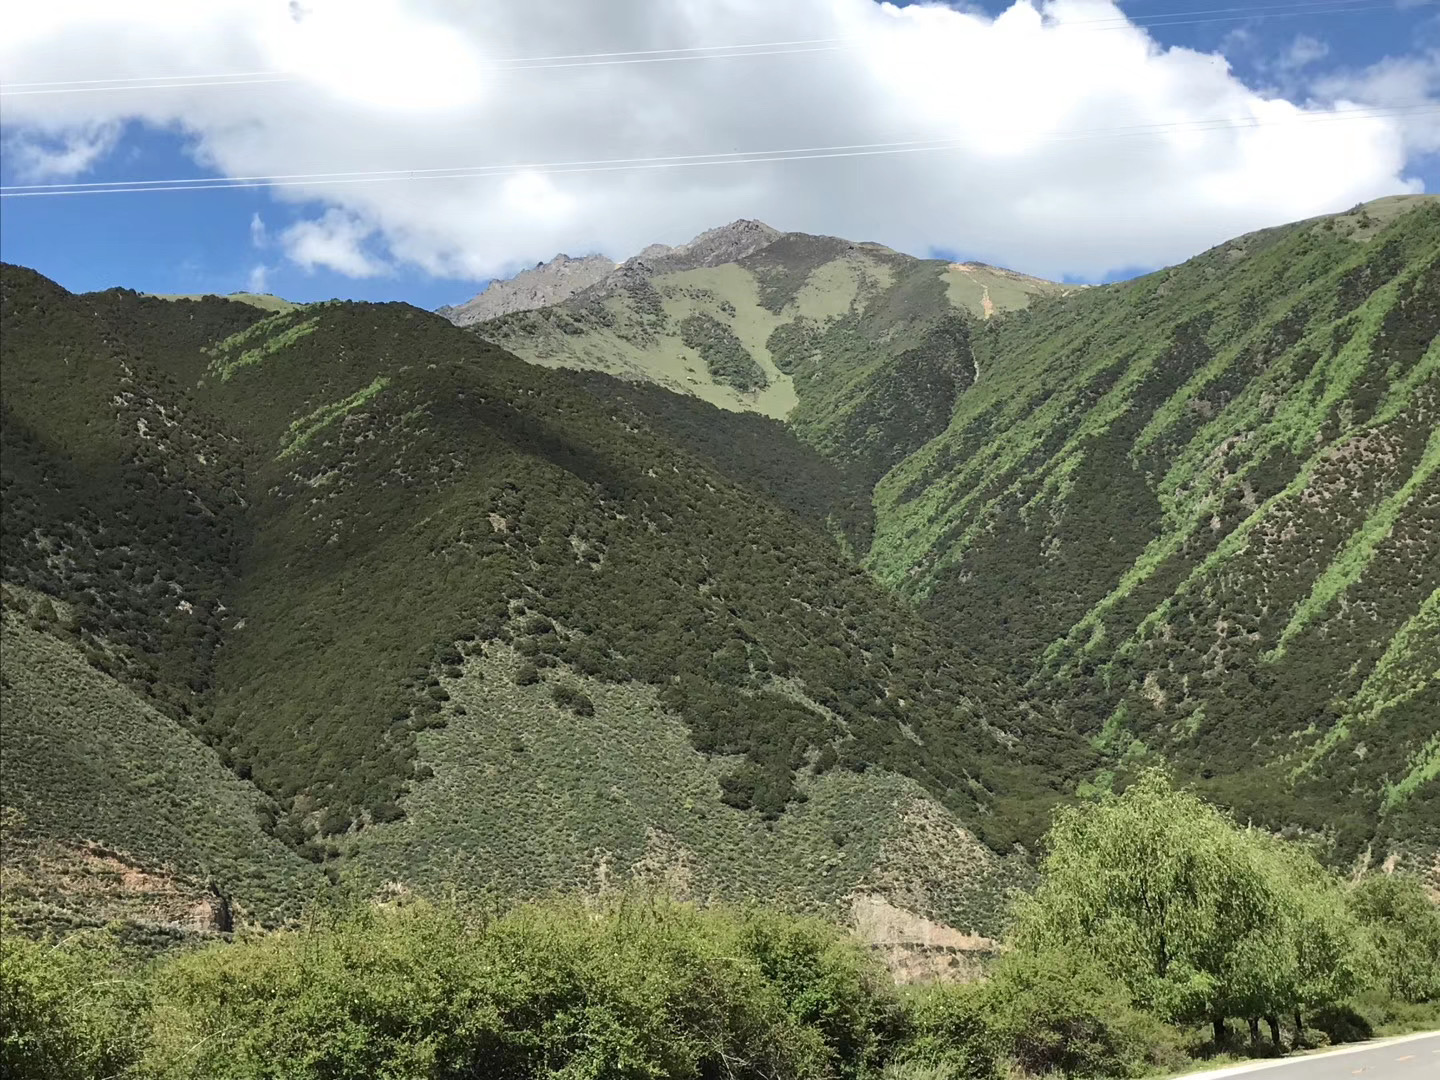
\includegraphics[keepaspectratio,
                                 width=\paperwidth]{images/cn_for_yu/IMG_0235.JPG}
            };
        \end{tikzpicture}
        \note[item]{China's Forests are Diverse}
     \end{frame}
}



{ % all template changes are local to this group.
    \setbeamertemplate{navigation symbols}{}
    \begin{frame}<article:0>[plain]
      \frametitle{}
        \begin{tikzpicture}[remember picture,overlay]
            \node[at=(current page.center)] {
                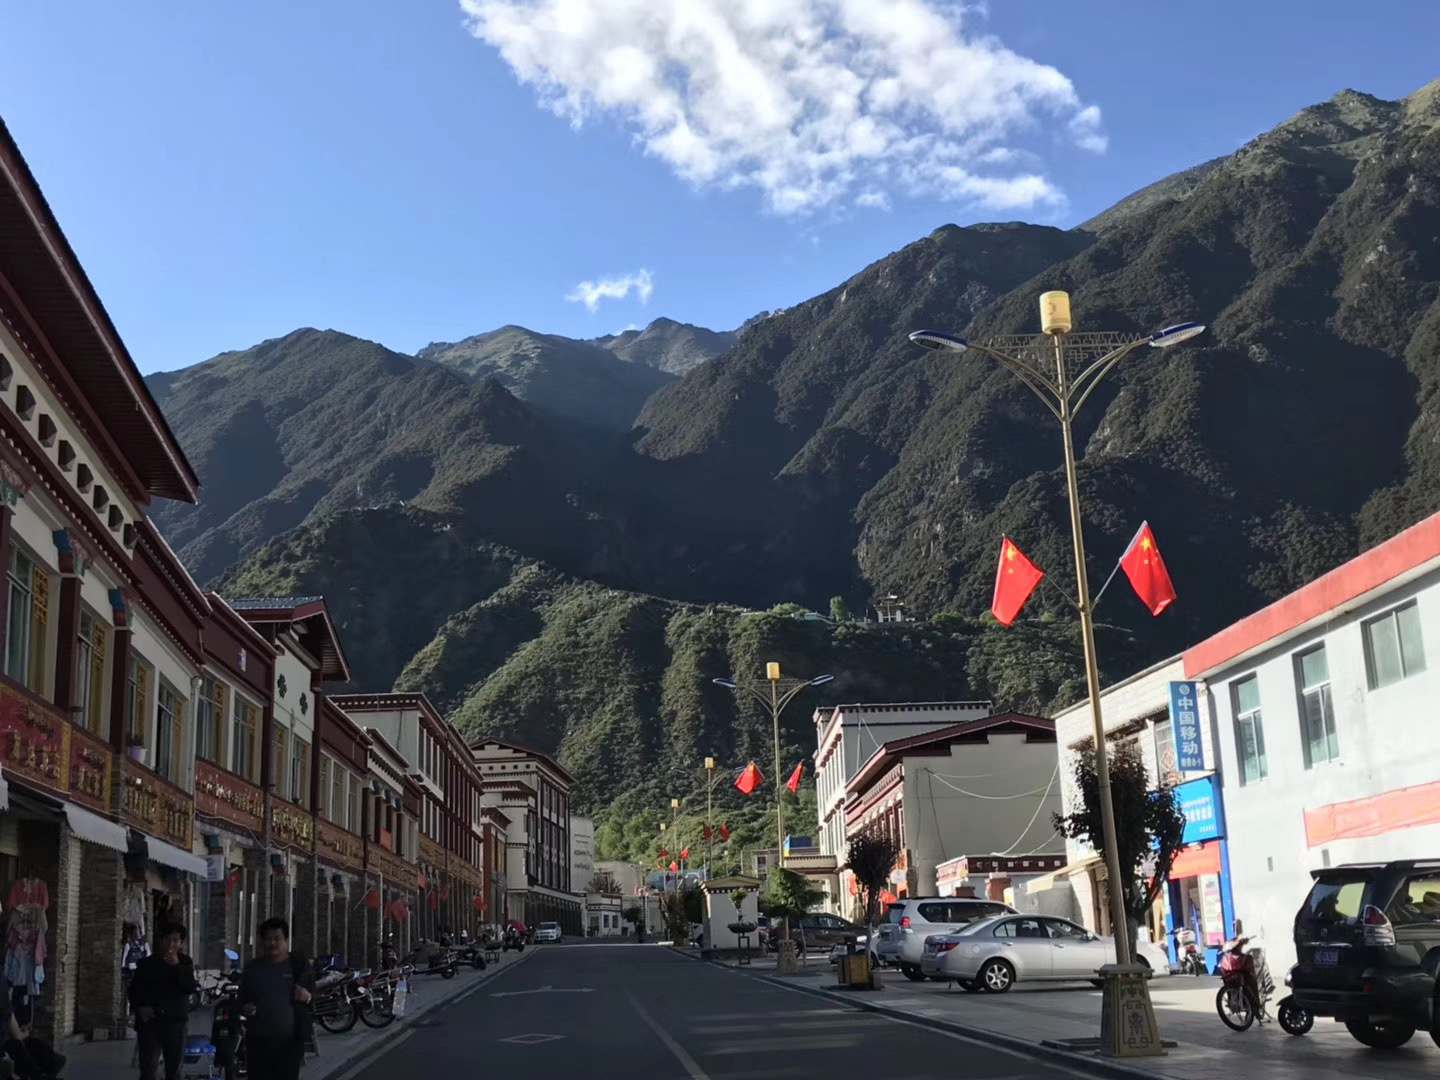
\includegraphics[keepaspectratio,
                                 width=\paperwidth]{images/cn_for_yu/IMG_0236.JPG}
            };
        \end{tikzpicture}
        \note[item]{China's Forests are Diverse}
     \end{frame}
}



{ % all template changes are local to this group.
    \setbeamertemplate{navigation symbols}{}
    \begin{frame}<article:0>[plain]
      \frametitle{}
        \begin{tikzpicture}[remember picture,overlay]
            \node[at=(current page.center)] {
                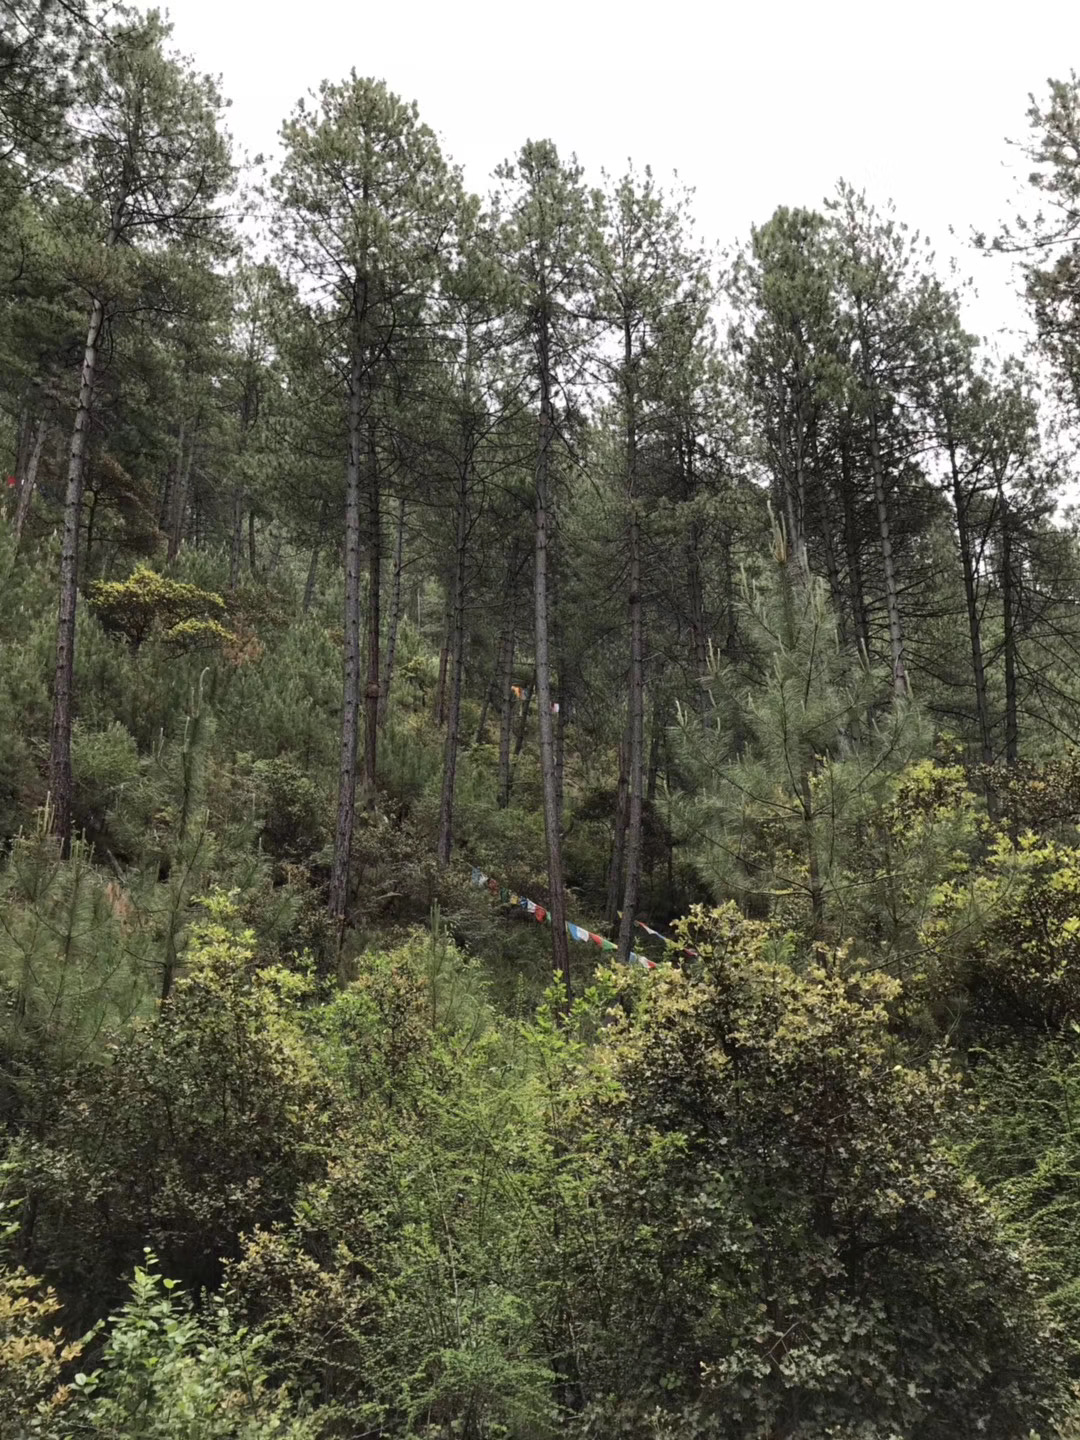
\includegraphics[keepaspectratio,
                                 width=\paperwidth]{images/cn_for_yu/IMG_0237.JPG}
            };
        \end{tikzpicture}
        \note[item]{China's Forests are Diverse}
     \end{frame}
}



{ % all template changes are local to this group.
    \setbeamertemplate{navigation symbols}{}
    \begin{frame}<article:0>[plain]
      \frametitle{}
        \begin{tikzpicture}[remember picture,overlay]
            \node[at=(current page.center)] {
                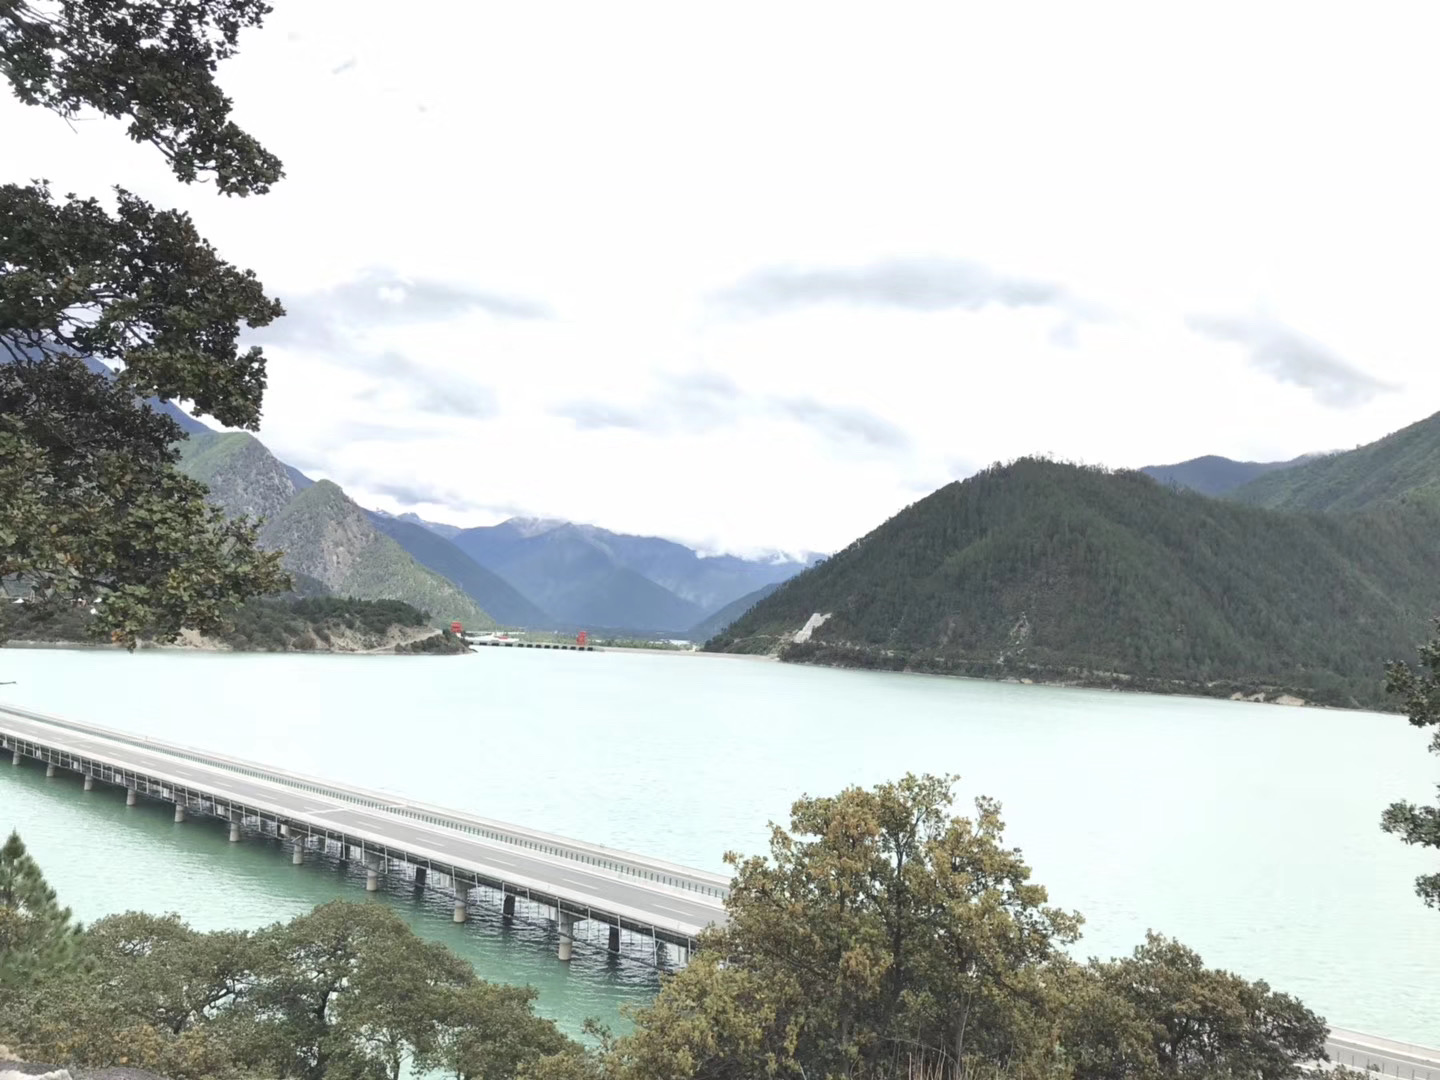
\includegraphics[keepaspectratio,
                                 width=\paperwidth]{images/cn_for_yu/IMG_0238.JPG}
            };
        \end{tikzpicture}
        \note[item]{China's Forests are Diverse}
     \end{frame}
}



{ % all template changes are local to this group.
    \setbeamertemplate{navigation symbols}{}
    \begin{frame}<article:0>[plain]
      \frametitle{}
        \begin{tikzpicture}[remember picture,overlay]
            \node[at=(current page.center)] {
                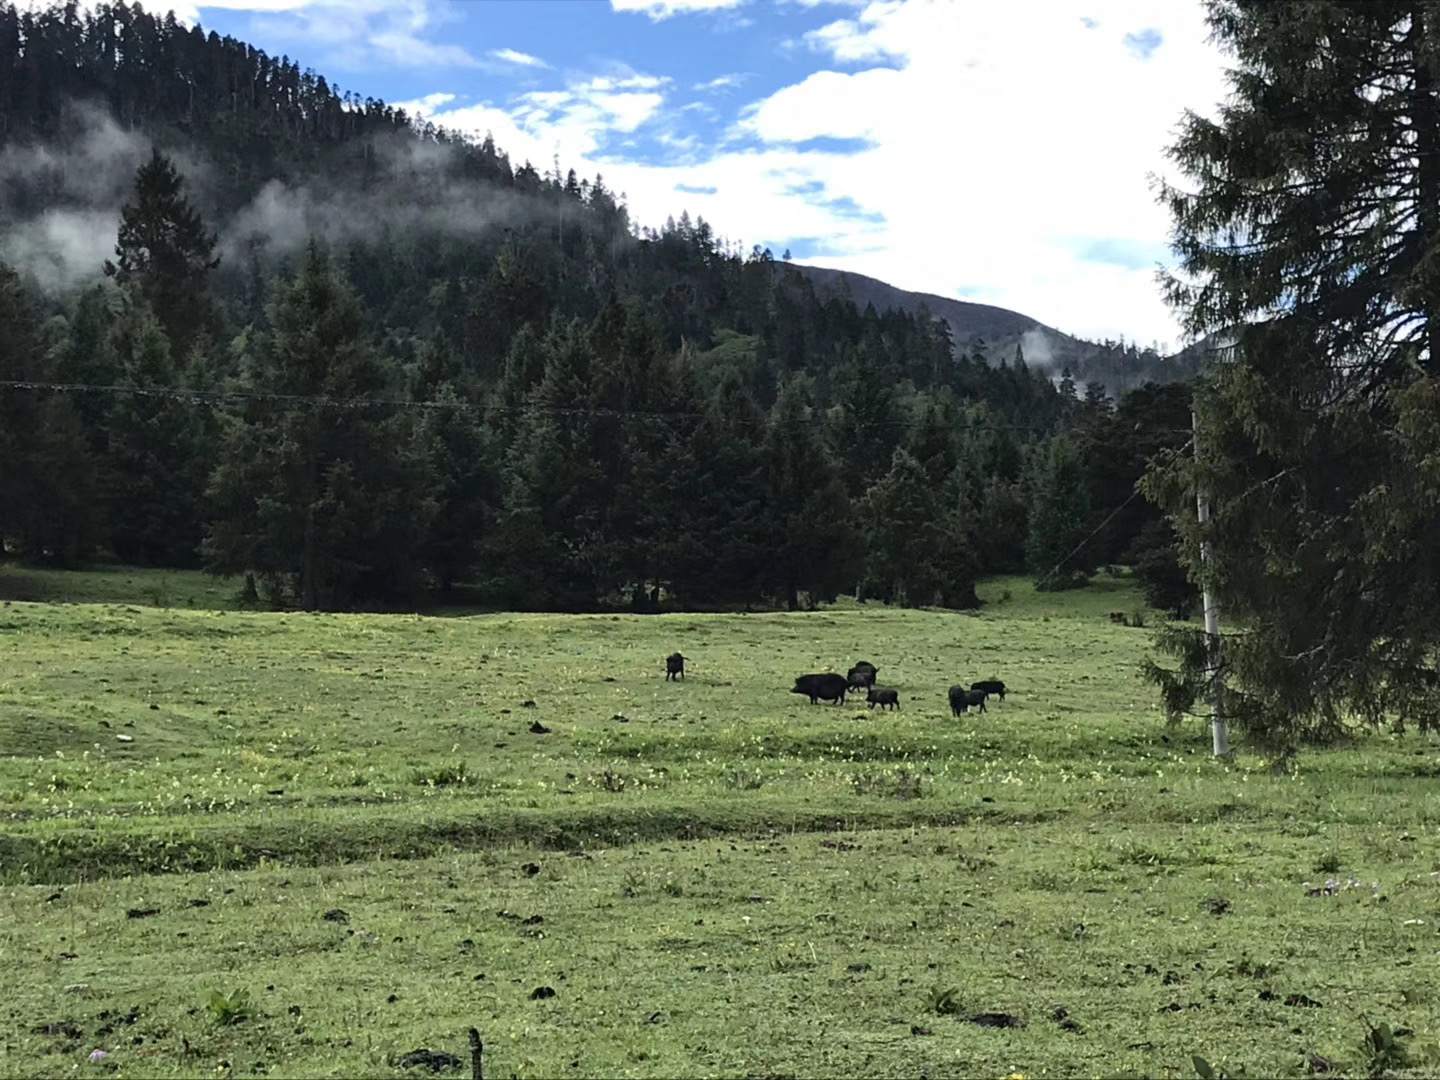
\includegraphics[keepaspectratio,
                                 width=\paperwidth]{images/cn_for_yu/IMG_0239.JPG}
            };
        \end{tikzpicture}
        \note[item]{China's Forests are Diverse}
     \end{frame}
}



{ % all template changes are local to this group.
    \setbeamertemplate{navigation symbols}{}
    \begin{frame}<article:0>[plain]
      \frametitle{}
        \begin{tikzpicture}[remember picture,overlay]
            \node[at=(current page.center)] {
                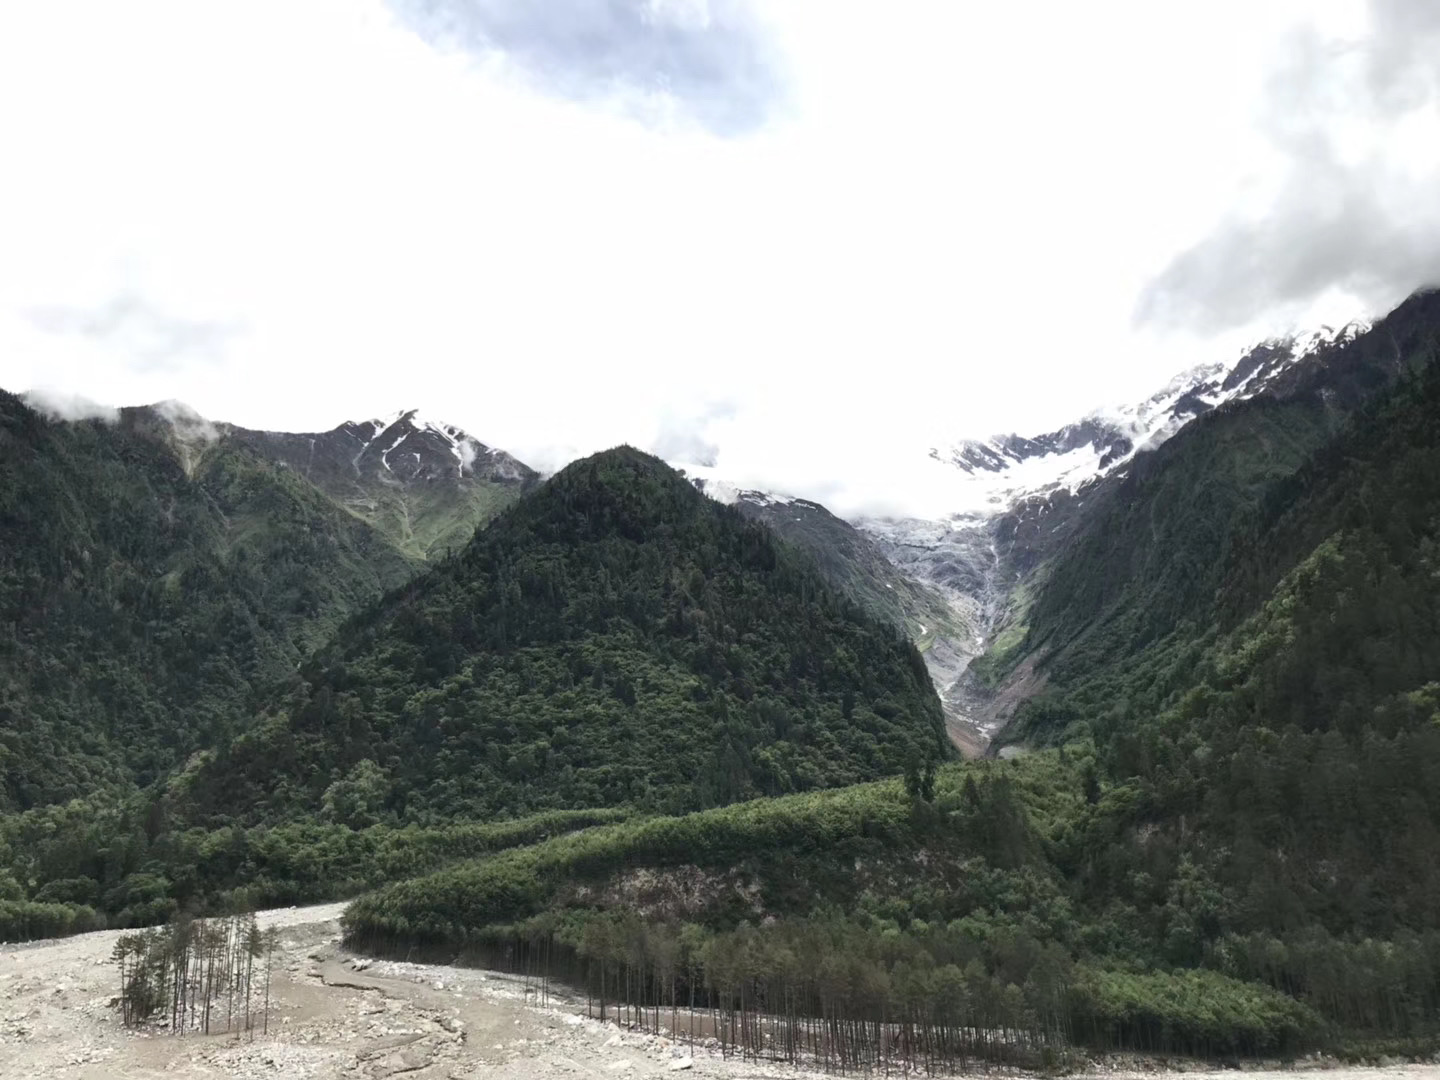
\includegraphics[keepaspectratio,
                                 width=\paperwidth]{images/cn_for_yu/IMG_0240.JPG}
            };
        \end{tikzpicture}
        \note[item]{China's Forests are Diverse}
     \end{frame}
}



{ % all template changes are local to this group.
    \setbeamertemplate{navigation symbols}{}
    \begin{frame}<article:0>[plain]
      \frametitle{}
        \begin{tikzpicture}[remember picture,overlay]
            \node[at=(current page.center)] {
                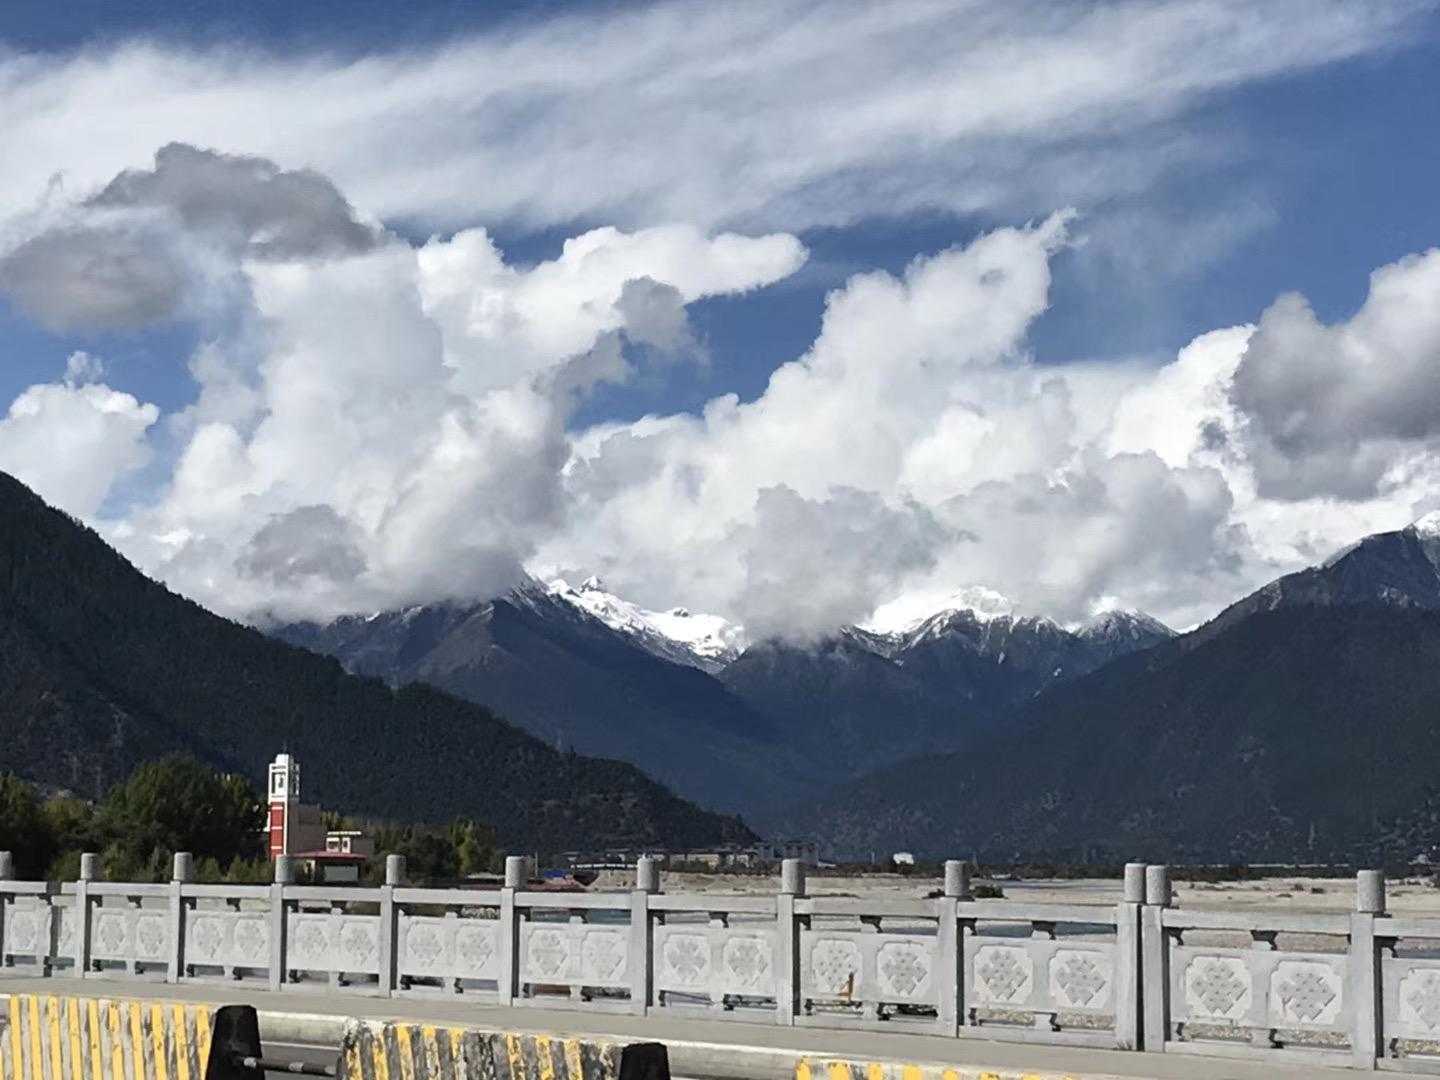
\includegraphics[keepaspectratio,
                                 width=\paperwidth]{images/cn_for_yu/IMG_0241.JPG}
            };
        \end{tikzpicture}
        \note[item]{China's Forests are Diverse}
     \end{frame}
}



{ % all template changes are local to this group.
    \setbeamertemplate{navigation symbols}{}
    \begin{frame}<article:0>[plain]
      \frametitle{}
        \begin{tikzpicture}[remember picture,overlay]
            \node[at=(current page.center)] {
                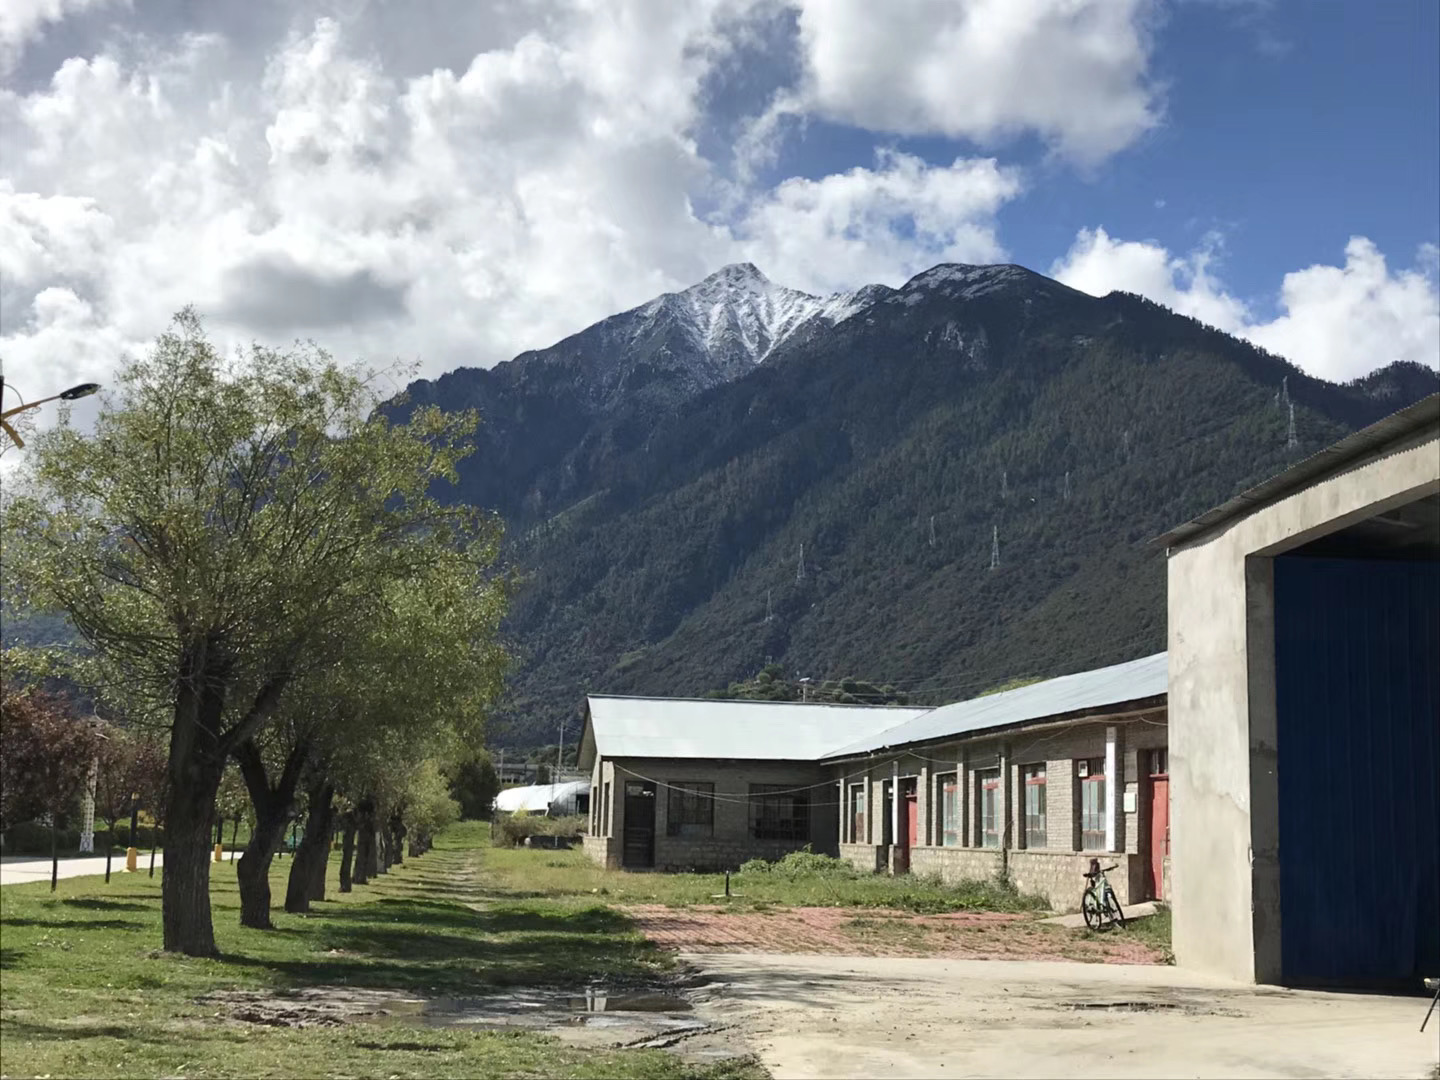
\includegraphics[keepaspectratio,
                                 width=\paperwidth]{images/cn_for_yu/IMG_0242.JPG}
            };
        \end{tikzpicture}
        \note[item]{China's Forests are Diverse}
     \end{frame}
}



{ % all template changes are local to this group.
    \setbeamertemplate{navigation symbols}{}
    \begin{frame}<article:0>[plain]
      \frametitle{}
        \begin{tikzpicture}[remember picture,overlay]
            \node[at=(current page.center)] {
                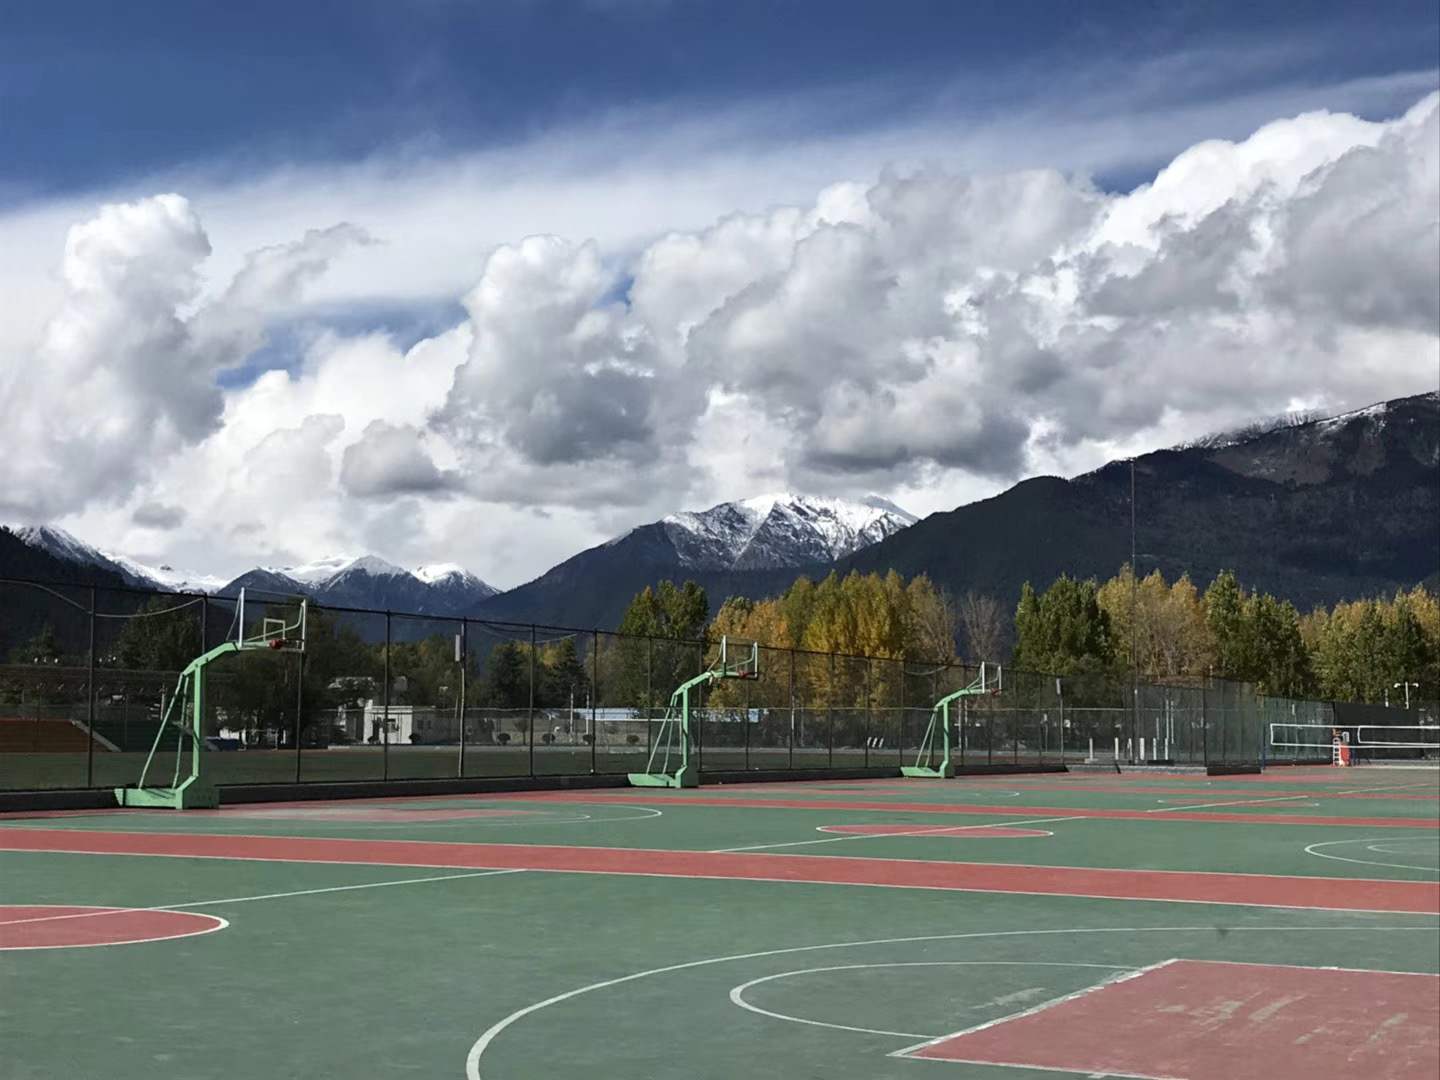
\includegraphics[keepaspectratio,
                                 width=\paperwidth]{images/cn_for_yu/IMG_0243.JPG}
            };
        \end{tikzpicture}
        \note[item]{China's Forests are Diverse}
     \end{frame}
}



{ % all template changes are local to this group.
    \setbeamertemplate{navigation symbols}{}
    \begin{frame}<article:0>[plain]
      \frametitle{}
        \begin{tikzpicture}[remember picture,overlay]
            \node[at=(current page.center)] {
                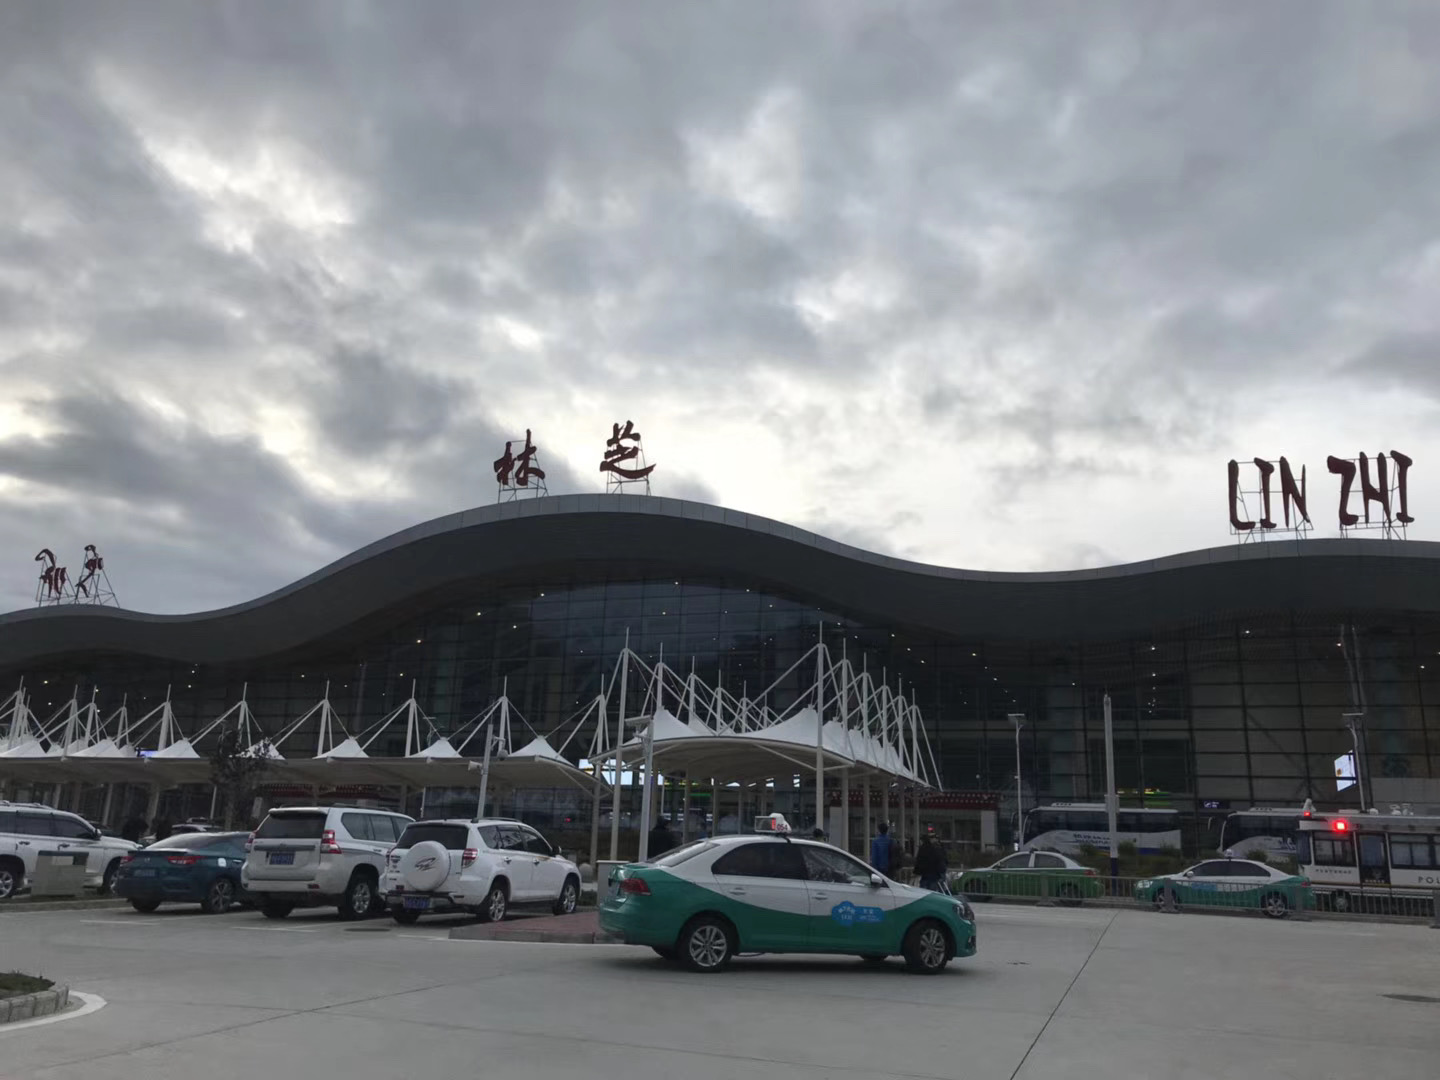
\includegraphics[keepaspectratio,
                                 width=\paperwidth]{images/cn_for_yu/IMG_0244.JPG}
            };
        \end{tikzpicture}
        \note[item]{China's Forests are Diverse}
     \end{frame}
}



{ % all template changes are local to this group.
    \setbeamertemplate{navigation symbols}{}
    \begin{frame}<article:0>[plain]
      \frametitle{}
        \begin{tikzpicture}[remember picture,overlay]
            \node[at=(current page.center)] {
                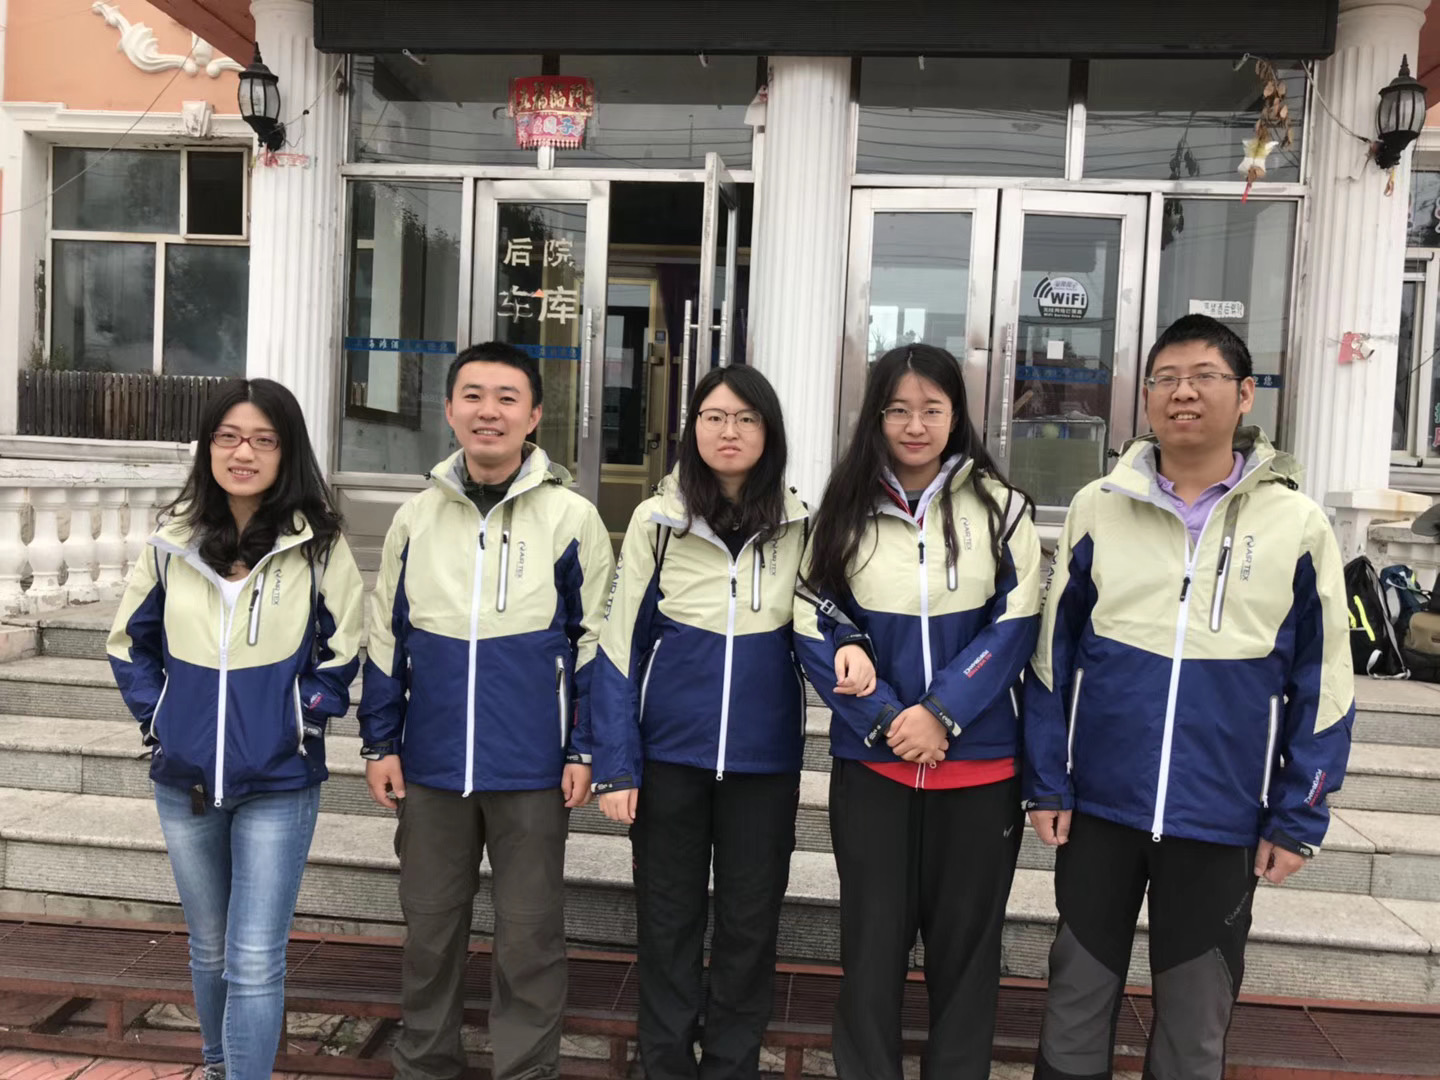
\includegraphics[keepaspectratio,
                                 width=\paperwidth]{images/cn_for_yu/IMG_0245.JPG}
            };
        \end{tikzpicture}
        \note[item]{China's Forests are Diverse}
     \end{frame}
}



{ % all template changes are local to this group.
    \setbeamertemplate{navigation symbols}{}
    \begin{frame}<article:0>[plain]
      \frametitle{}
        \begin{tikzpicture}[remember picture,overlay]
            \node[at=(current page.center)] {
                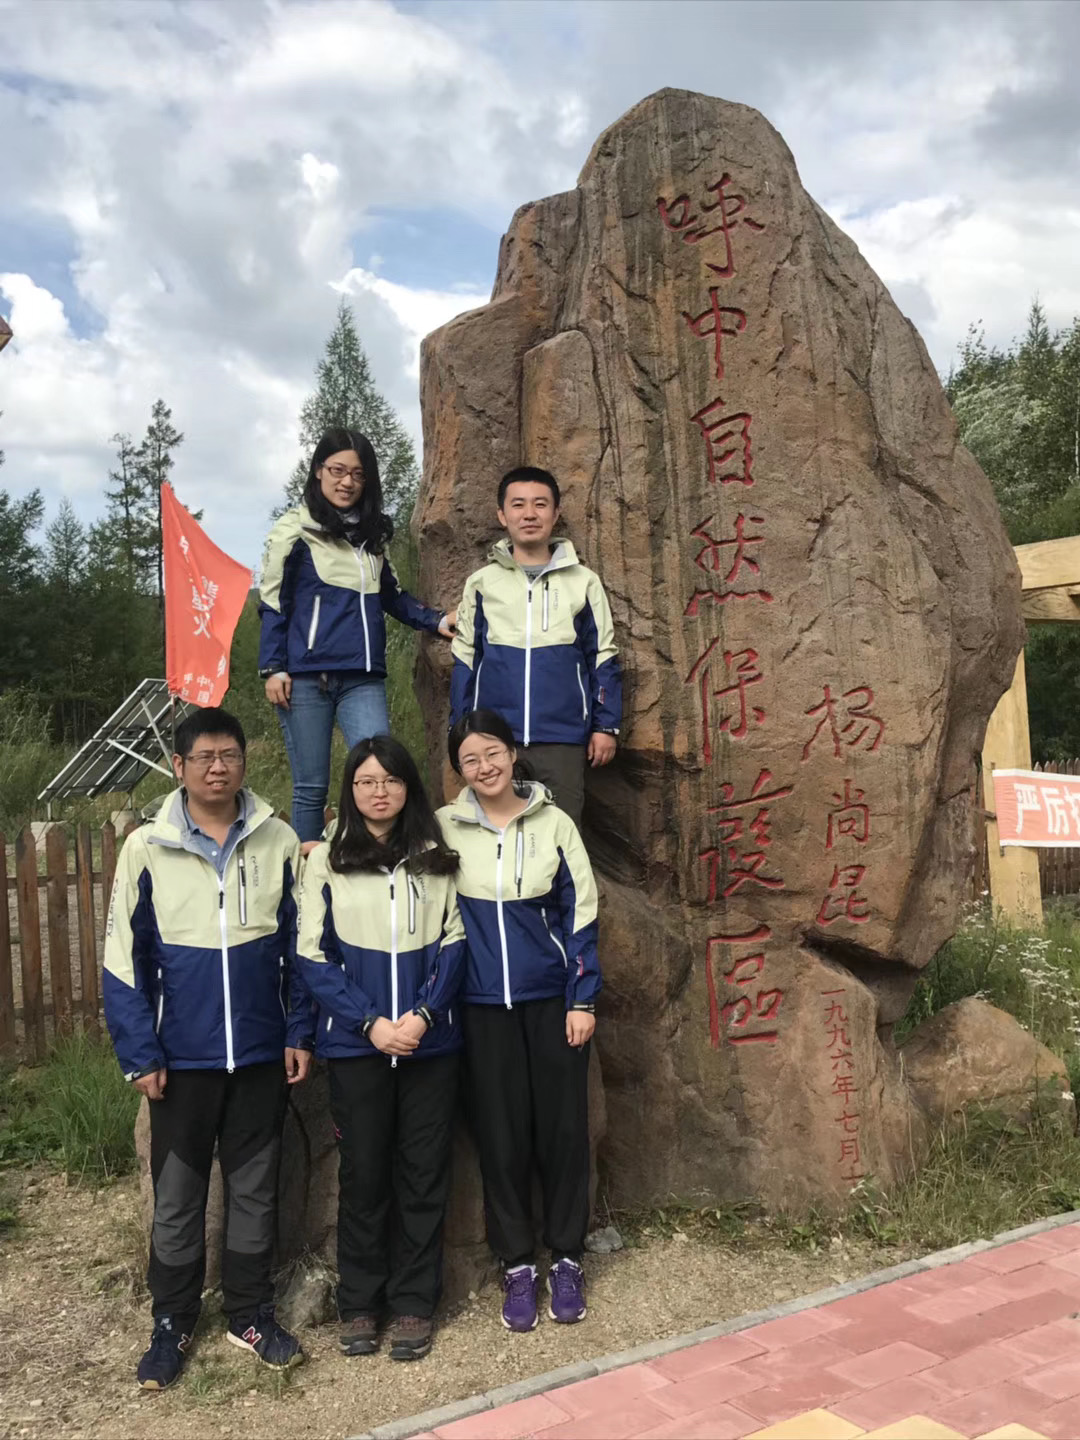
\includegraphics[keepaspectratio,
                                 width=\paperwidth]{images/cn_for_yu/IMG_0246.JPG}
            };
        \end{tikzpicture}
        \note[item]{China's Forests are Diverse}
     \end{frame}
}



{ % all template changes are local to this group.
    \setbeamertemplate{navigation symbols}{}
    \begin{frame}<article:0>[plain]
      \frametitle{}
        \begin{tikzpicture}[remember picture,overlay]
            \node[at=(current page.center)] {
                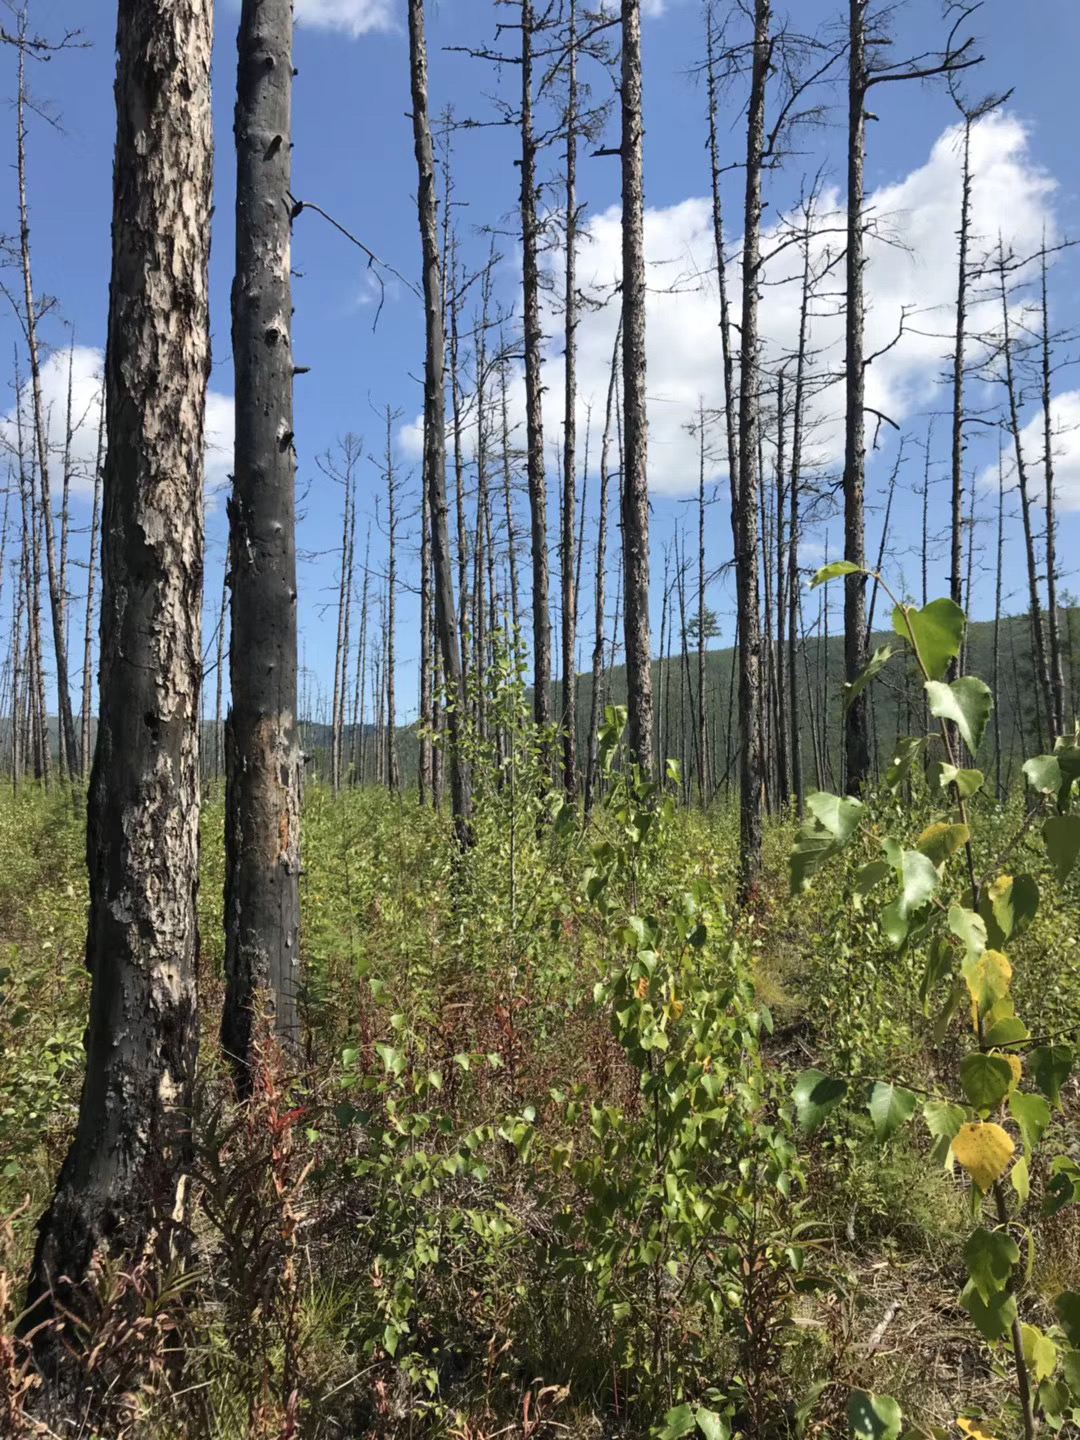
\includegraphics[keepaspectratio,
                                 width=\paperwidth]{images/cn_for_yu/IMG_0247.JPG}
            };
        \end{tikzpicture}
        \note[item]{China's Forests are Diverse}
     \end{frame}
}



\begin{frame}
  \frametitle{China's Forest Networks: Global}
\end{frame}


\begin{frame}
  \frametitle{China's Forest Networks: Domestic/Local}
\end{frame}

%%   - Local Scale
%% 	- Landscape = Chen 2019
%% 	- Resilience Analysis of China's Forest LE-MRIO

\section{Conclusions}

\begin{frame}
  \frametitle{Conclusions}
\end{frame}

\section{Future Work}

\begin{frame}
  \frametitle{Future Work}
\end{frame}


\begin{frame}
  \frametitle{Future Work}
\begin{columns}
\begin{column}{0.5\textwidth}
    \begin{center}
     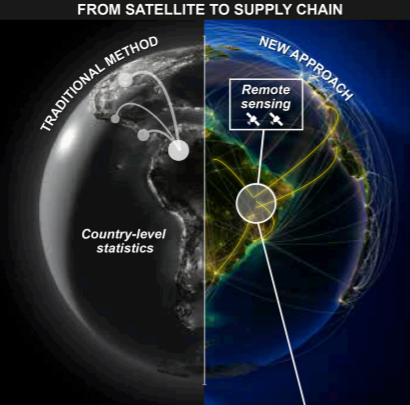
\includegraphics[width=0.86\textwidth]{images/moran_2020_1.png}
     \end{center}
\end{column}
\begin{column}{0.5\textwidth}  %%<--- here
    \begin{center}
     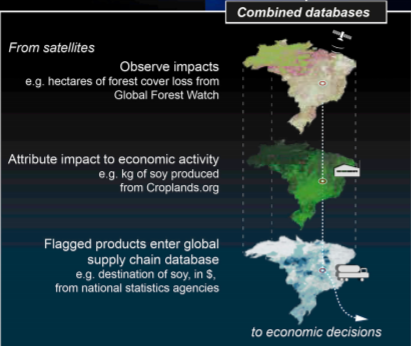
\includegraphics[width=1.0\textwidth]{images/moran_2020_2.png}
     \end{center}
\end{column}
\end{columns}
\end{frame}


\begin{frame}
  \frametitle{Acknowledgements}
\end{frame}



{ % all template changes are local to this group.
    \setbeamertemplate{navigation symbols}{}
    \begin{frame}<article:0>[plain]
      \frametitle{}
        \begin{tikzpicture}[remember picture,overlay]
            \node[at=(current page.center)] {
                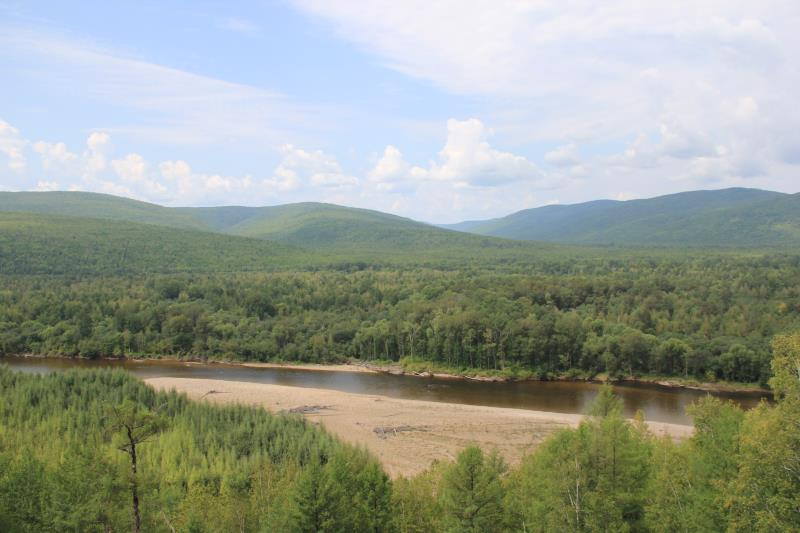
\includegraphics[keepaspectratio,
                                 width=\paperwidth]{images/CNF/IMG_0199.JPG}
            };
        \end{tikzpicture}
        \note[item]{Questions, comments?}
     \end{frame}
}

\begin{frame}
  \cite{Burgess2012}    
  \cite{Caggiani2014}
  \cite{Carvalho2019AdaptationSystems}
  \cite{Schaffer-Smith2018NetworkTrade}
\end{frame}


\begin{frame}[allowframebreaks]
  \frametitle{References}
  \tiny \bibliography{biblio.bib}
  \bibliographystyle{abbrv}
\end{frame}


\end{document}
